\documentclass[11pt,twopage]{article}
%%%%%%%%%%%%%%%%%%%%%%%%%%%%%%%%%%%%%%%%%%%%%%%%%%%%%%%%%%%%%%%%%%%%%%%%%%%%%%%%%%%%%%%%%%%%%%%%%%%%%%%%%%%%%%%%%%%%%%%%%%%%%%%%%%%%%%%%%%%%%%%%%%%%%%%%%%%%%%%%%%%%%%%%%%%%%%%%%%%%%%%%%%%%%%%%%%%%%%%%%%%%%%%%%%%%%%%%%%%%%%%%%%%%%%%%%%%%%%%%%%%%%%%%%%%%
\usepackage{amssymb}
%\usepackage[round]{natbib}
\usepackage[round]{natbib}
\usepackage{makeidx}
\usepackage{graphicx,amssymb}
\usepackage{caption}
\usepackage{subcaption}
\usepackage{amsmath}
\usepackage{a4,latexsym,amsmath,amstext,graphicx,amssymb}
\usepackage{amsthm}
\usepackage{bbm}
\usepackage{color}

% %
%\usepackage{setspace}

\PassOptionsToPackage{hyphens}{url}\usepackage{hyperref}
%\usepackage{hyperref}


% turn on comments:
\newcommand{\mycomment}[1]{\textbf{[#1]}}
\newcommand{\AN}[1]{\textcolor{red}{[AN: #1]}}
\newcommand{\AS}[1]{\textcolor{blue}{[AS: #1]}}
\newcommand{\PX}[1]{\textcolor{green}{[PX: #1]}}

% turn off comments:
%\newcommand{\mycomment}[1]{}
%\newcommand{\AN}[1]{}
%\newcommand{\AS}[1]{}
%\newcommand{\PX}[1]{}


\setcounter{MaxMatrixCols}{10}


\DeclareMathOperator{\owhom}{OWHOM}
\DeclareMathOperator{\poly}{poly} \DeclareMathOperator{\dlog}{DL}
\DeclareMathOperator{\image}{img} \DeclareMathOperator{\prob}{Pr}
\DeclareMathOperator{\IF}{IF} \DeclareMathOperator{\ELSE}{ELSE}
\DeclareMathOperator{\NP}{NP} \DeclareMathOperator{\DEXP}{DEXP}
\DeclareMathOperator{\DMEXP}{DMEXP}
\DeclareMathOperator{\DPOW}{DPOW}
\DeclareMathOperator{\DMEXPPOW}{DMEXP-POW}
\DeclareMathOperator{\GSROOT}{GSROOT}
\DeclareMathOperator{\desc}{desc}
\newcommand{\ol}{\overline}
\newcommand{\ul}{\underline}
%\newenvironment{hypothesis}[Hypothesis]
\newtheorem{claim}{Claim}
{\bf}{\it}
\newtheorem{ourproblem}{Problem}
{\bf}{\it}
\newtheorem{problem}{Problem}
{\bf}{\it}
\newtheorem{assumption}{Assumption}
{\bf}{\it}
\newtheorem{definition}{Definition}
{\bf}{\it}
\newtheorem{proposition}{Proposition}
{\bf}{\it}
\newtheorem{remark}{Remark}
{\bf}{\it}
\newtheorem{lemma}{Lemma}
{\bf}{\it}
\newtheorem{theorem}{Theorem}
{\bf}{\it}
\newtheorem{corollary}{Corollary}
{\bf}{\it}
\newtheorem{conjecture}{Hypothesis}
{\bf}{\it}
\textwidth=450pt \textheight=610pt \marginparwidth=0pt
\topmargin=0pt \marginparsep=0pt \oddsidemargin=10pt
\evensidemargin=10pt
\newcommand{\draft}[1]{}
\newcommand{\be}{\begin{equation}}
\newcommand{\ee}{\end{equation}}
\newcommand{\bes}{\begin{equation*}}
\newcommand{\ees}{\end{equation*}}
\newcommand{\bea}{\begin{eqnarray}}
\newcommand{\eea}{\end{eqnarray}}
\newcommand{\beas}{\begin{eqnarray*}}
\newcommand{\eeas}{\end{eqnarray*}}

\begin{document}

\title{Foreclosure Auctions} \author{
  \\
  Andras Niedermayer\\
  {University of Mannheim}\\
  \\
  Artyom Shneyerov\\
  {Concordia University, CIREQ, CIRANO}\\ \\
  Pai Xu\\
  {University of Hong Kong, Hong Kong} }

\date{This Draft: \today}

\thispagestyle{empty}
\maketitle

\begin{abstract}

  We develop a novel theory of real estate foreclosure auctions, which
  have the special feature that the lender acts as a seller for low
  and as a buyer for high prices. The theory yields several
  empirically testable predictions concerning the strategic behavior
  of the agents, both under symmetric and asymmetric
  information. Using novel data from Palm Beach County (FL, US), we
  find evidence of both strategic bidding and asymmetric information,
  with the lender being the informed party. Moreover, the data are
  consistent with mortgage securitization leading to moral hazard with
  respect to banks' effort in collecting information about the value
  of the mortgage collateral.

%
  % We get two predictions: (i) lenders' bids are bunched at the
  % amount owed, (ii) in the presence of a common value component the
  % probability of selling to a third-party bidder is non-monotone and
  % discontinuous in the lender's maximum bid. Using novel data from
  % Palm Beach County (FL, US), we show that (i) and (ii) are
  % consistent with the data. Further, our theory and our data allow
  % us to confirm the wide-held suspicion that lenders of securitized
  % mortgages are less informed than lenders of non-securitized
  % mortgages.  Our theory also allows a welfare analysis of judicial
  % versus non-judicial foreclosures.
\end{abstract}

\setlength{\baselineskip}{1.5\baselineskip}
% \doublespacing

\noindent \textbf{Keywords: } foreclosure auctions, common value component, securitization \\
\textbf{JEL Codes: } to be added


\section{Introduction}

Foreclosures of real estate have a substantial economic impact. In
2013, 609,00 residential sales in the U.S. were foreclosure related
(foreclosure auctions or sales of real estate owned by a lender),
amounting to 10.3\% of total residential sales.\footnote{See
  \url{http://www.realtytrac.com/Content/foreclosure-market-report/december-and-year-end-2013-us-residential-and-foreclosure-sales-report-7967}.}

Foreclosures played an even larger role during the 2007 and 2008
financial crisis, when "four million families [...] lost their homes
to foreclosure and another four and a half million [...] slipped into
the foreclosure process or are seriously behind on the mortgage
payments" \cite[p. xv]{angelides2011financial}. The foreclosure wave had
a strong connection to the securitization of mortgages: the rate of
securitization of subprime mortgages increased from 46 per cent in
2001 to 81 per cent in 2006 \cite[p. 19]{dewatripont2010balancing}. It is widely
believed that the securitization of mortgages led to moral hazard on
the side of originating banks and that "collapsing mortgage-lending
standards and the mortgage securitization pipeline lit and spread the
flame of contagion and crisis" \cite[p. xxiii]{angelides2011financial}.

We develop a novel theory of foreclosure auctions, incorporating the
institutional specificities of foreclosures. Our theory serves both a
better understanding of the foreclosure process and, as it will become
apparent later, also provides insight about the moral hazard involved
in securitization. A foreclosure auction is run by a government agency
(in our data set the Clerk and Comptroller's Office of Palm Beach
County, FL) after a mortgagee stopped making payments to the
lender. The lender, typically a bank, and third-party bidders,
typically real estate brokers, participate in this auction. An
important feature of foreclosure auctions is that payments up to the
amount owed (the judgment amount) are paid to the lender, payments
above the judgment value, if any, are paid to the owner of the
property. The owner typically does not participate. In such an
auction, the bank essentially acts as a seller below the judgment
amount, and as a buyer above the judgment amount.

Another important feature of foreclosure auctions is that the bank is
likely to have superior information about the value of the mortgage
collateral being auctioned off. There are several reasons for
this. First, lenders typically spend large resources on appraisals to
get a more precise value of the collateral before granting
mortgages. %\AN{cite stroebel} 
Second, banks also typically put
significant effort in assessing the probability of default of
potential borrowers. The probability of default is well known to be
negatively correlated with the value of the collateral \cite[see][and the references therein]{qi2009loss}. Hence, the bank's signal about
the financial soundness of the borrower also serves as a signal for
the value of the property.

In contrast to the bank, which is mostly interested in reselling the
property and may have superior information about quality, brokers
typically participate with the intent of renovating the
property.\footnote{When visiting websites of several brokers
  participating in the foreclosure auctions in our dataset, we could
  see that they often specialize in renovating foreclosed properties.}
The costs of renovation are to a much larger degree driven by
idiosyncratic components. Hence, it is a reasonable approximation to
assume private values on the brokers' side.\footnote{Assuming private
  values also helps us to focus on the common value component on the
  seller's side, which has been ignored so far in the empirical
  literature. Our theoretical results are likely to extend to a setup
  in which buyers also have information about the common value
  component. However, such a setup would add much more complexity to
  our model than in standard auction models, due to the complexity of
  a common value component on the seller's side and the change of
  incentives at the judgment amount. Further, for a better
  understanding of moral hazard in the securitization process, what
  matters is the common value component on the seller's side.}

% The brokers' expected payoffs depend both of the bank's information
% and on their own idiosyncratic components (signals). The latter may
% reflect their own value added to the property.\footnote{When
% visiting websites of several brokers participating in the
% foreclosure auctions in our dataset, we could see that they often
% specialize in renovating foreclosed properties.} This value added
% may be largely independent of the baseline value of the house, so we
% assume that the broker and bank signals are independent. The
% relevance of the bank's information to the broker creates a common
% value component in the auction. However, unlike the standard common
% value model where buyers have relevant information, here is it
% assumed that only the bank is the informed party.

We derive participants' equilibrium bidding strategies in a
foreclosure auction with a common value component. However, as a
benchmark, we first analyze a symmetric information environment, where
the bank's information is known to the brokers. This independent
private value (IPV) setup is nested within our general model. Under
IPV, brokers bid their own type as in a standard English auction. The
bank bids its valuation plus a markup for valuations far below the
judgment amount, just as a seller would bid. The bank's bid takes into
account the classical trade-off of a seller: a higher bid lowers the
bank's probability of selling the house, but increases the bank's
revenue in case of sale. However, one side of this trade-off
disappears for banks that bid exactly the judgment amount: a higher
bid still lowers the probability of sale, but does not lead to higher
revenues for the bank, since the additional revenue goes to the
original owner. This change of the trade-off causes a bunching of
banks' bids at the judgment amount. If the bank's valuation is
sufficiently high -- higher than the judgment amount- the bank does
not want to sell the property, but would want to keep it
itself. Hence, for high valuations, the bank bids its own type, just
as a buyer would do in an English auction.

A bank intent on selling the property will bid more in an asymmetric
information environment than in a symmetric information environment
(the \emph{signalling premium}). The reason is that there is a further
effect in the bank's trade-off: the bank's bid also serves as a costly
signal about the quality of the property. Intuitively speaking, the
bank is willing to incur the cost of an excessively low probability of
sale (given the price conditional on sale), in order to prove that the
quality of the house is high. This cost has to be sufficiently high,
so that bank's with lower qualities do not have an incentive to
imitate banks with lower qualities.

Additionally to the signalling premium, one still has the bunching
result from the symmetric information setup. However, bunching has a
surprising implication in the presence of a common value component:
there cannot be an equilibrium where the bank's biding strategy is
continuous around the bunch. The reason for this is that brokers who
are supposed to drop slightly below the judgment amount will instead
prefer to wait for the price to rise above the judgment amount, as
they would then be certain to obtain a significantly higher house
quality at a slightly higher price. Since brokers will not have an
incentive to drop out at prices slightly below the judgment amount,
neither will have the bank: increasing the bid to the judgment amount
will lead to a higher revenue for the bank, while not changing the
probability of selling. This logic implies that there has to be a
discontinuity in the bank's bidding strategy below the judgment
amount. We show that the bank's equilibrium bidding strategy is
strictly increasing and continuous for low valuations, exhibits a
discontinuous jump to the judgment amount and bunching at the judgment
amount, and is equal to the bidding strategy of a buyer for valuations
above the judgment amount.


Our theory has two striking empirically testable implications. First,
there is bunching of banks' bids at the judgment amount the judgment
amount. Second, in the presence of both auctions with symmetric and
asymmetric information, one should expect to observe the
following. For values slightly below the judgment amount, the
probability of sale (the probability of the bank selling the house to
a third-party bidder) first increases with the bank's bid and then
drops down discontinuously at the judgment amount. The explanation for
this consists of two pieces. First, with asymmetric information there
is a gap in the bank's bid distribution just below the judgment amount
(corresponding to the discontinuous bidding strategy), whereas for
symmetric information there is no gap. Hence, bids observed just below
the judgment amount will be from symmetric information auctions. For
other bids, one will observe a mixture of symmetric and asymmetric
information. Second, the signalling premium leads to higher bids by
the bank and hence a lower probability of sale for asymmetric
information than symmetric information. Putting the two pieces
together reveals that the probability of sale will be lower in the gap
than just below and just above the gap. This implies a probability of
sale which is non-monotonic with the bank's bid at the lower bound of
the gap and decreases discontinuously at the upper bound of the gap
(which is the judgment amount).\footnote{If there are only two types
  of auctions, auctions with symmetric information and one type of
  auction with asymmetric information, there will also be a
  discontinuity at the lower bound of the gap, so that there would be
  two discontinuities. However, only the upper discontinuity is robust
  to multiple types of asymmetric auctions: for all auctions with
  asymmetric information, the upper bound of the gap is at the
  judgment amount. However, the lower bound of the gap will be
  different. This will smooth out the discontinuity at the lower
  bounds of the gaps, but not the discontinuity at the judgment
  amount.} This \emph{non-monotonicity} (which appears like a
violation of the law of demand) and \emph{demand discontinuity} are
empirically testable implications of our theory.


% This is due to the following selection effect. For prices slightly
% below the judgment amount, the symmetric information auctions are
% selected into the observable sample. This is because there is a
% \emph{gap} in the bank's bids below the judgment amount under
% asymmetric information. For prices at and slightly above the
% judgment amount, both symmetric and asymmetric information auctions
% are selected. As the probability of sale (``demand") is lower under
% asymmetric information due to the signalling premium, the observable
% demand will exhibit a downward jump at the judgment amount. Further,
% for bank's bids just below the judgment amount, the probability of
% sale increases with the bank's bid. The reason is that the closer
% the bank's bid approaches the judgment amount from below, the more
% one gets a selection into symmetric information auctions. This
% selection leads to a higher observed probability of sale, because of
% the aforementioned signalling premium in the asymmetric information
% auctions. This \emph{demand discontinuity} and
% \emph{non-monotonicity} due to the selection effect are testable
% predictions in the environment where both symmetric and asymmetric
% information auctions are present.

% The probability of sale (i.e. the probability that a realtor wins
% the auction) decreases with the seller's reserve price for prices
% far below and far above the judgment amount. However, just below and
% just above the judgment amount, the probability of sale
% \emph{increases} with the price, this effect being due to a
% selection effect.

To bring our theory to the data, we have collected a novel data set
with foreclosure auctions from Palm Beach County in Florida. We have
data on 12,788 auctions from 2010 to 2013 with a total judgment amount
of \$4.2bn and a total sale amount (the sum of the winning bids) of
\$0.5bn. The data reveal that bunching indeed occurs at the judgment
amount. We also observe that the probability of sale increases with
the bank's bid just below the judgment amount. Further, demand
exhibits a downward discontinuity at the judgment amount. This points,
as we have argued, to the presence of auctions with both symmetric and
asymmetric information in our dataset.

% As we have argued, the distinguishing feature of the asymmetric
% information environment is the signalling premium. Controlling for
% the value of the house, we should expect the bank to bid higher
% under symmetric information. But at the same time, we have also
% argued that our sample contains both symmetric and asymmetric
% information auctions. Nevertheless, we are able to address the
% signalling premium directly by looking separately at
% \emph{securitized} mortgages, where, as we shall argue, the bank may
% not have superior information. By estimating the bidding strategies
% for securitized and non-securitized mortgages, we can empirically
% verify the presence of the signalling premium.

% Further empirical support for asymmetric information is provided by
% considering securitized and non-securitized mortgages.
%
% As we have argued, asymmetric information leads to a signalling
% premium in bidding. By comparing securitized and non-securitized
% mortgages, we are able to show the existence of a signalling premium
% directly, thus providing further empirical support for the existence
% of asymmetric information in foreclosure auctions.

Our theory and our data allow us to investigate moral hazard in the
securitization process.  The securitization of mortgages was a major
concern during the financial crisis.  Originating banks securitized
their mortgages through securitization agencies (mostly the Government
Sponsored Enterprises Freddie Mac and Fannie Mae), the securitized
assets were then sold on the capital market. Moral hazard is generally
believed to have played an important role during the financial crisis:
banks did not exert sufficient effort in gathering information before
granting mortgages and hence excessively granted mortgages and
securitized them, shifting the burden to the holders of securitized
assets and Government Sponsored Entities (and often ultimately to the
taxpayer) \cite[see][]{mian2009consequences,dewatripont2010balancing,keys2008did}.

The connection between moral hazard at the stage of granting a
mortgage and asymmetric information at the time of the foreclosure is
the following. In the presence of moral hazard for securitized
mortgages, a bank will exert less effort in collecting information
both about the value of the collateral and the financial situation of
the borrower. One effect of this is that the bank will be less
informed about the probability of default -- this is indeed what the
literature has focused on so far. However, there is also a second
effect: once a mortgage defaults, the loss given default (and hence
the value of the collateral) matters. If the originating bank spent
less effort gathering information about the value of the collateral
when granting the mortgage, it will also have less of an informational
advantage during the foreclosure auction.

% Different levels of information gathering for securitized and
% non-securitized mortgages have empirically testable implications for
% foreclosure auctions: a bank holding a non-securitized mortgage is
% expected to be better informed about the value of the property than
% a bank holding a securitized mortgage. This is for two
% reasons. First, the bank is more likely to have gathered information
% about the loan-to-value ratio of a property for non-securitized
% mortgages. Second, the bank's estimate of the probability of default
% of a borrower is informative about the value of the property at the
% time of the foreclosure (see \cite{qi2009loss}). A reason for the
% relation between the probability of default and the value of the
% property is that borrowers in financial distress are less likely to
% invest in the maintenance of their property.\footnote{Causality can,
% of course, also go in the opposite direction: home owners with a
% higher loan-to-value ratio have more of an incentive to default. For
% our purposes, it is immaterial in which direction the causality
% goes. In either case, superior information about the probability of
% default also leads to superior information about the value of the
% property.} % [ADD SOME
% CITATIONS HERE]

% We can divide the foreclosure auctions into those related to a
% securitized mortgage and those related to a non-securitized
% mortgage.
One would therefore expect the bank to have less private information
about the quality of the house for securitized mortgages than for
non-securitized mortgages. This implies that the non-monotonicity and
the discontinuity of the probability of sale as a function of the
bank's bid should be present for non-securitized mortgages, but not
for securitized mortgages (or at least only present to a smaller
extent). An analysis of the data reveals that this is indeed the case.

We provide further evidence for banks having less of an informational
advantage for securitized than for non-securitized mortgages by
considering bank's bidding strategies. Because of the signalling
premium, a bank bids higher under asymmetric than under symmetric
information given the same opportunity cost of selling.\footnote{We
  show for a linear utility specification of our theory a stronger
  result: the bank's bid increases with the degree of informational
  asymmetry. In the linear utility specification, a parameter $\alpha$
  is the weight of the bank's signal in the utility of a third party
  bidder. $\alpha=0$ means independent private values, an increase of
  $\alpha$ can be interpreted as an increase of informational
  asymmetry. Our result is that the bank's bid increases with
  $\alpha$.} In order to estimate banks' bidding strategies for
securitized and non-securitized mortgages and to correct for possible
selection effects,\footnote{A different distribution of banks' bids
  for securitized and non-securitized mortgages could be either due to
  the signalling premium or due to banks having a different
  distribution of opportunity costs for securitized and
  non-securitized mortgages.} we collected additional data on the
resale prices and the tax assessment values of foreclosed
properties. These two additional variables allow us to deal with the
selection effect while taking care of unobserved heterogeneity. This
allows us to estimate banks' bidding functions for securitized and
non-securitized mortgages. We show that for a given opportunity cost,
a bank holding a non-securitized mortgage bids more than a bank
holding a securitized mortgage. This provides additional evidence for
different levels of asymmetric information at the foreclosure stage
and hence moral hazard at the stage of granting mortgages.

% Next, we consider a version of our model where the broker's
% valuation depends on the bank's information \emph{linearly}, with
% coefficient $\alpha$ measuring the degree of bank's
% informativeness. A higher $\alpha$ corresponds to more precise
% information concerning the common value component. We show that the
% bank will bid more aggressively if $\alpha$ is higher. This is
% \emph{both} because of the direct effect on the broker values, and
% the indirect effect due to the higher incentive to signal the
% favourable information to the brokers.
%
% We provide direct evidence that asymmetric information plays a
% bigger role for the foreclosure auctions of non-securitized by
% showing that the signalling premium is larger.  In order to be able
% to estimate the bank's bidding strategy, we collected additional
% data on the resale prices and the tax assessment values of
% foreclosed properties. Using the resale price and the assessment
% value as two independent noisy signals for banks' valuations, we
% constructed the distribution of banks' valuations for securitized
% and non-securitized mortgages. Matching the quantiles of banks'
% valuation distributions with banks' bid distributions gives us the
% (average) bidding function. Having an estimate of the bidding
% function for both securitized and non-securitized mortgages, we show
% that for a given valuation, a bank holding a non-securitized
% mortgage bids more than a bank holding a securitized mortgage. This
% is consistent with asymmetric information being more salient for
% non-securitized mortgages.

% This information asymmetry has potentially important implications
% for securitization policies. As we explain, these policies have
% traditionally focused on the probability of default, in particular
% as measured by the borrower's FICO score. However, the total cost of
% a defaulted mortgage will also include the loss given default. The
% latter is determined by the value of the house recovered in the
% foreclosure auction. It is this total loss that gets insured by the
% US federal mortgage agencies, with the cost ultimately borne by the
% taxpayer. We find that (i) the bidding behavior of the lenders is
% consistent with the hypothesis that they are likely to be better
% informed when the mortgage is not securitized, and (ii) the recovery
% ratio is substantially lower in the pool of the securitized
% mortgages. Taken together, these findings suggest that some of the
% original lender's informational advantage concerning the recovery
% value of the mortgage is already present at the securitization
% stage. This information is likely to be private, leading to a
% previously unrecognized dimension of adverse selection at the
% securitization stage.

% The first finding is important because it indicates that the banks
% are likely to have \emph{private} information concerning the loss
% given default already at the securitization stage, effectively
% transferring this loss to the taxpayers. The second finding is
% important because it indicates that this information is likely to be
% privately known by the bank. This points towards a potentially
% important and previously unrecognized market failure at the
% securitization stage, and the potential need for a policy response
% to address it.


% There is also a generally held suspicion that lower quality
% mortgages are securitized and sold on the market, despite the fact
% that securitization agencies screen based on publicly observable
% characteristics. The suspicion is that securitized mortgages are
% worse with respect to characteristics which cannot be observed
% publicly. However, it is in the nature of characteristics that
% cannot be publicly observed that it is difficult to make empirical
% statements concerning them. With our theory giving clear predictions
% on what one should observe with and without a common value
% component, we can look in more detail at the question whether for
% non-securitized mortgages banks indeed have private information of
% the quality of the house. The data for securitized mortgages seems
% to be more consistent with an independent private values setup,
% whereas for non-securitized mortgages, it is more consistent with
% there being a common value component for one part of the auctions.

%
% What are the welfare implications of common values and the
% associated adverse selection in foreclosure auctions? Building on
% the insights in \cite{cai2007reserve}, \cite{jullien2006auction} and
% \cite{lamy}, we show that seller bids in the foreclosure auction
% under common values involve a \emph{signalling premium} for bids
% below the judgment amount. That is, they are higher relative to what
% they would have been if the realtors knew the bank's
% information. This introduces a further distortion, on top of the
% usual deadweight loss stemming from the bank's monopoly position as
% the seller. Fro the bids above the judgment amount, on the other
% hand, there is no distortion, as the bank will act as a buyer, and
% the English auction will allocate the house efficiently.


%
%
%
% Under the assumption that for non-judicial foreclosures the same
% buyers with the same valuations participate in an auction, we can
% make a welfare comparison between judicial and non-judicial
% foreclosures. Under an independent private values setup, judicial
% foreclosures generate higher welfare than non-judicial
% foreclosures. A comparison in a common values setup is work in
% progress.
%
\paragraph{Related Literature.} To the best of our knowledge, this is
the first paper providing an economic analysis of the bidding behavior
in foreclosure auctions. So far, the details of foreclosure auctions
have been mainly analyzed in the law literature (see
e.g. \cite{nelson2004reforming}).

For our theoretical analysis, we build on two strains of
literature. The first analyzes bidding behavior of buyers with
information about a common value component, starting with
\cite{milgrom1982theory}. The second, more recent, literature analyzes
auctions in which the seller has superior information, see
\cite{jullien2006auction}, \cite{cai2007reserve}, \cite{lamy}. For
bids above the judgment amount, we can use results from the former;
for bids sufficiently below the judgment amount, we can use results
from the latter literature, in particular from
\cite{cai2007reserve}. Our theoretical contribution is to show that
there are surprising predictions for the intermediate range of bids,
which are between the informed seller and the informed buyer regions.

To the best of our knowledge, this is also the first paper to provide
empirical evidence for a common value component \emph{on the seller's
  side} in an auction. In this sense, it complements the existing
empirical auction literature, which has focused on a common value
component on the \emph{buyer's side}, see
\cite{hendricks1988empirical} and \cite{hendricks2003empirical} for
offshore oil auctions, and \cite{nyborg2002bidder} and
\cite{hortaccsu2012valuing} for treasury auctions.

Our setup makes it particularly easy to find a common value component
on the seller's side. This is because (i) participation in the sales
is required by law and (ii) the seller is a private
organization. Without (i) (i.e. with voluntary participation)
submarkets with particularly strong adverse selection would operate at
a low scale or might even completely break down by an
\cite{akerlof1970market} type of argument. Hence, if one cannot
perfectly separate submarkets with symmetric and asymmetric
information, there is a selection effect working against finding
asymmetric information.\footnote{It is plausible that one cannot
  perfectly separate different submarkets. At least in our data set,
  we find evidence consistent with both symmetric and asymmetric
  information auctions being present.} Point (ii) matters, because
governments are less likely to have superior information. Much of the
literature has analyzed markets in which either (i) or (ii) was not
satisfied, hence even if one had looked for a common value component on
seller's side rather than the buyer's side, it would have been difficult 
to find it.

% Evidence of strategic behavior and asymmetric information has long
% been a focus of the empirical auction literature, beginning with
% \cite{hendricks1988empirical} and \cite{hendricks2003empirical} for
% offshore oil auctions, and \cite{nyborg2002bidder} and
% \cite{hortaccsu2012valuing} for treasury
% auctions. \cite{hortaccsu2012valuing} find evidence of dealers'
% informational advantage in Canadian Treasury auctions.

% Recently, \cite{stroebel2013asymmetric} has provided evidence of
% asymmetric information concerning the collateral value in mortgage
% lending. \cite{stroebel2013asymmetric} finds that integrated lenders
% have superior information about the quality of the houses they lend
% against, and this information allows them to reduce the probability
% of foreclosure by as much as $40\%$.

The application of our theory to securitization relates to the
literature dealing with moral hazard, such as \cite{mian2009consequences}, \cite{keys2008did},
\cite{tirole2011illiquidity}. Our analysis provides
further evidence that securitization led to moral hazard. Our analysis
is complementary to the analysis in the existing literature that
provides evidence for moral hazard with respect to the probability of
default. Our analysis shows moral hazard with respect to the other
determinant of the expected shortfall of a mortgage: the loss given
default (which is determined by the value of the mortgage collateral).

In a wider sense, our article relates to the growing literature that
uses insights from auctions to analyze important questions in
financial markets, such as \cite{heller1998auctions},
\cite{hortacsu2010mechanism}, \cite{cassola20132007},
\cite{zulehner2013competition}, albeit for the analysis of
mortgages rather than treasury bills.


\section{Foreclosure Process}
Property foreclosure is a remedy allowed by law to the lender if the
borrower defaults on the mortgage. While it generally transfers the
ownership of the property to the lender, the process may be a lengthy
one and the details depend on the jurisdiction. In the US, roughly
$40\%$ of the states adopt what is called a \emph{judicial}
foreclosure, while the rest is comprised of the \emph{nonjudicial}
foreclosure states. See Figure \ref{fig:judicial}.\footnote{This and
  other information concerning judicial and nonjudicial foreclosures
  can be found in \cite{nelson2004reforming}.}


The main legal difference between judicial and nonjudicial foreclosure
is that in the former, the process takes place in the court system,
while in the latter, it takes place outside the courts. Judicial
foreclosures always result in the property being sold at a public
auction, while the nonjudicial foreclosure usually involves a sale of
the property by the trustee under the power of sale clause. The
trustee sale may or may not be conducted through auction, but still
have to generally comply with various state laws, even though it is
performed outside of the court system.\footnote{A handful of states
  (Connecticut, Maine and Vermont) allow for a \emph{strict
    foreclosure}, where the property title is transferred to the
  lender immediately after the default.}

\begin{figure}[t]
  \centering
  \includegraphics{graphics/foreclosure_map}
  \caption{States with judicial and non-judicial foreclosures}
  \label{fig:judicial}
\end{figure}

In this paper, we focus on judicial foreclosures. In our empirical
application, we study foreclosure auctions in a judicial state
(Florida). The judicial foreclosure process generally consists of the
following steps.\footnote{These steps are described in relative detail
  at e.g.\ \url{www.nolo.com}.}

\begin{enumerate}
\item The mortgage holder misses several payments on the mortgage. In
  some states, the lender is allowed to start the foreclosure process
  after the borrower has missed one payment. In practice, however, the
  process usually begins after three payments have been missed.
\item The lender informs the mortgage holder, usually through a letter
  of intent with a specified deadline, that it intends to begin the
  foreclosure process. This notice of intent, or ``breach letter",
  allows the borrower to make up the missed payments before the
  deadline. The deadline is usually set at 30 days.
\item If the mortgage is still delinquent, the lender proceeds to file
  a lawsuit, usually in the county where the property is located. The
  complaint is served to the mortgagee, usually by the county
  sheriff. At this point, the mortgagee becomes a defendant in the
  foreclosure lawsuit.
\item The defendant is given a certain amount of time, usually 20 - 30
  days, to respond. The defendant does not have to respond. The
  defendant may choose to respond if he or she is able to raise a
  substantive complaint, e.g.\ concerning the ownership of the
  mortgage or unfair lending practices.
\item If the complaint goes uncontested or the defendant does not
  raise a substantive complaint, the lender is granted a judgment of
  foreclosure. The judgment will specify the date of the foreclosure
  sale. The sale is conducted through a public auction. The bank is
  allowed to credit bid up to the debt amount (also called the
  judgment amount), while other participants (usually real estate
  brokers) are required to submit bids in cash or cash equivalent. The
  auction is usually conducted in an open format. Some counties have
  adopted Internet auctions.\footnote{This is the case for Palm Beach
    county in Florida, the source of the data for the empirical
    application in our paper.} The property title is awarded to the
  highest bidder, and the auction price is equal to the highest
  bid. If the lender is \emph{not} the highest bidder, the lender
  receives the payment equal to the minimum of the auction price and
  the judgment amount. If the sale price exceeds the judgment amount,
  the surplus is used to satisfy the junior liens, if any. The
  remaining surplus is paid to the defendant.\label{enum:auction}
\end{enumerate}



In the next section, we present a stylized model of the terminal stage
of the foreclosure process, the foreclosure auction.


\section{Model}

Consider the owner, the bank (also called the seller, $S$) and $n$
real estate brokers (or buyers, $B$) who participate in the
foreclosure auction. The judgment amount (i.e.\ the balance of the
mortgage) is denoted as $v_J$. The foreclosure auction is modelled as
variant of the (button) English auction as in
\cite{milgrom1982theory}. The auction website expedites bidding by
allowing the participants to employ automatic bidding agents. The
bidders provide their agents the maximum price they are willing to pay
(their \emph{dropout} price), and the agent then bids on their
behalf. These proxy bids can be updated at any time.\footnote{Such
  proxy bidding makes the button model even more applicable here, as
  it alleviates the need to model difficult features such as e.g.\
  jump bidding that may be present in the traditional open auctions.}
The brokers are able to observe if the bank's maximum bid has been
exceeded, while a broker's dropout price is unobservable to the
bank. The broker may therefore change its maximum bid upon observing
the bank's dropout price. As for the bank, we assume that it commits
to its dropout price.

The key difference from a standard auction is that the proceeding of
the foreclosure auction up to the judgment amount goes to the bank,
anything above the judgment amount goes to the original owner. This
effectively turns the bank into a seller for prices below and into a
buyer for prices above the judgment amount.

The winner pays the auction price $p$.  If the price exceeds the
judgment amount, $p\geq v_J$, then the bank gets $v_J$ and the owner
pockets the difference $p - v_J$. If the price is below the judgment
amount, $p<v_J$, then the banks gets $p$ and the owner gets
nothing. The property is transferred to a broker only if a broker
wins; otherwise, the bank keeps the property. It follow that if the
bank wins the auction, it effectively pays the auction price to
itself, so in reality no money changes hands in this case. But if a
broker wins, then there is an actual money transfer, from the broker
to the bank and possibly the owner as well (if the auction price
exceeds the judgment amount).

As is usual, we model the foreclosure sale (auction) as a game of
incomplete information.  As is explained in the empirical section of
the paper, banks and brokers buy houses for different purposes: banks
mostly sell the houses later on. Brokers typically renovate the
property before reselling. Motivated by this, we make the following
assumption concerning the information of the bank and the
brokers. First, we assume that the $i$th broker's idiosyncratic
signal, denoted as $X_B^i$, only concerns its renovation value added
to the house. Second, we assume that the bank's signal $X_S$ concerns
the baseline resale value of the house. The signals $X_B^i$ and $X_S$
will be sometimes referred to as buyers' and seller's
\emph{types}. Their realizations will be denoted as $x_B^i$ and $x_S$,
respectively.

% Given the different nature of the bank's and broker's signals, it is
% assumed that $x_B^i$'s and $x_S$ are independent.
The bank is assumed to be the informed party. Its signal $X_S$ is
normalized to equal the expected value of the house in the market, so
the bank's valuation is
\[
u_S(x_S) = x_S .
\]
The brokers do not observe $X_S$; they only privately observe their
own signals $X_B^i$. Broker $i$'s expected value of the house, given
its own signal $x_B^i$ and the bank's signal $x_S$, is denoted as $
u_B(x_B^i,x_S).$


% To capture the fact that input prices may be correlated across the
% brokers, we allow the signals $x_B^i$ to be correlated.
%
%% They, however, have information about an additional idiosyncratic
%% component of their valuations, which is incorporated in the
%% broker's signal $x_B^i$.  $x_B$ can be thought of as the renovation
%% value of the house.
%
% We make the following assumptions about the buyer valuations. We
% assume that the distributions $F_B$ and $F_S$ are potentially
% different. The reason is that banks and brokers buy houses for
% differentnt purposes: banks mostly sell the houses later on. Brokers
% typically renovate the property before reselling.



We make the following assumptions concerning the expected valuations
of the brokers.

\begin{assumption}[Broker valuations]\label{as:valuations}
  A broker's expected valuation is differentiable and strictly
  increasing in own signal $x_B$, and nondecreasing in the bank's
  signal $x_S$,
  \begin{align}
    \frac{\partial u_B(x_B,x_S)}{\partial x_B}\geq \alpha,\quad
    \frac{\partial u_B(x_B,x_S)}{\partial x_S} \geq 0, \nonumber
  \end{align}
  for some constant $\alpha>0$.  Moreover, the derivatives satisfy the
  \emph{single crossing} condition
  \begin{align}
    \frac{\partial u_B(x_B,x_S)}{\partial x_B}>\frac{\partial
      u_B(x_B,x_S)}{\partial x_S} \nonumber
  \end{align}

  % and
  % \begin{align}
  %   u_B(x,x) = x.\label{eq:normalization}
  % \end{align}
  \label{as:utilities}
\end{assumption}




This assumption ensures that a broker's valuation of the house is
increasing in its own signal $x_B$, and is non-decreasing in the
bank's signal $x_S$. If $u_B$ does not depend on $x_S$, we have a
special case of \emph{private values}. Otherwise, the valuations are
interdependent.



For reasons that will be clear in the sequel, we normalize the broker
signals so that the value conditional on winning the auction is equal
to the signal,
\begin{align}
  u_B(x_B,x_B) = x_B.
  \label{bnorm}
\end{align}
This normalization is without loss of generality because Assumption
\ref{as:valuations} ensures that $u_B(x_B,x_B)$ is continuous and
strictly increasing in $x_B$.

We make the following assumptions regarding the distribution of the
signals.
\begin{assumption}[Signals]\label{as:info}
  The bank's signal $X_S$ is drawn from a distribution $F_S$ supported
  on $\mathbb R_{+}$, with density $f_S$ continuous and positive on
  the support. The broker signals $X_B^i$, $i=1,...,n$, are
  identically and independently distributed and drawn from the
  distribution $F_B$, supported on $\mathbb R_{+}$, with density $f_B$
  continuous and positive on the support.  \medskip
\end{assumption}
% We assume that the signals are independent.
% \begin{assumption}[Independence]
%   \noindent
% \end{assumption}
The independence assumption is made to simplify the analysis of the
game, by eliminating the need to consider adjustments that brokers
would otherwise make to their proxy bids following dropouts by other
brokers. Under independence, we shall see that the information in the
auction will be transmitted only from the bank to the brokers,
following the bank's dropout from the auction. After that, the brokers
would essentially have independent private values, and simply enter
those values as their (updated) proxy bids, and there will be no
updating from brokers' dropout prices.\footnote{Independence is also
  assumed in \cite{jullien2006auction}, while \cite{cai2007reserve}
  and \cite{lamy} allow the buyer signals to be correlated, but still
  independent of the seller's signal.}

The \emph{Myerson virtual value} is defined in the present setting as
\begin{align} J_B(x_B,x_S) = u_B(x_B,x_S) -\frac{\partial
    u_B(x_B,x_S)}{\partial x_B} \frac{1-F_B(x_B)}{f_B(x_B)}.
\end{align}
We make the standard monotonicity assumption concerning
$J_B(x_B,x_S)$.
\begin{assumption}[Virtual value monotonicity] \label{as:myerson} The
  function $J_B(x_B,x_S)$ is strictly increasing in $x_B$.
\end{assumption}

In the following, we will use $x_{(1)}$ and $x_{(2)}$ for the highest
and second highest order statistics among $n$ brokers'
signals. Further, we will use $F_{(1)}$ and $F_{(2)}$ for the
corresponding distributions.

We have to reasons to focus on a model in which the seller's superior
information about the quality of the property being auctioned is at
the center of interest. First, the bank is likely to have better
information due to having gathered information about the property when
granting the mortgage. Information about the mortgagee can also serve
as an indication of how well the mortgagee maintains the
house. Second, we will later consider securitized and non-securitized
mortgages. As it will become clearer later on, there are reasons to
believe that the informativeness of the bank's signal about the
quality of the house is different for securitized and non-securitized
mortgages.

\section{Symmetric information}
\label{sec:indep-priv-valu}

It is useful to first start with the case of \emph{symmetric
  information}, where the bank's information is known to the brokers.
This independent private values (IPV) setup is particularly useful to
highlight the role of the judgment amount, below which the bank acts
as a seller and above which the bank acts as a buyer.

% Under IPV, our normalization implies \[u_B(x_B,x_S) = x_B,\] and the
% Myerson virtual value here is simply \[ J_B(x_B) = x_B -
% \frac{1-F_{B}(x_B)}{f_{B}(x_B)}. \]
Standard arguments imply that it is a weakly dominant strategy for the
broker to choose its valuation as the drop out price, so
\[p_B(x_B) = x_B.
\]
% \begin{remark}
%   If buyer signals are independent, or, by convention, if there is
%   only one buyer, $J_B(\cdot)$ becomes the standard Myerson virtual
%   value, \[ J_B(x_B) = x_B - \frac{1-F_{B}(x_B)}{f_{B}(x_B)} .\]
% \end{remark}

The bank's bidding behavior can be best derived by first considering
two hypothetical cases. First, nothing is owed to the bank ($v_J=0$)
and hence the bank always acts as a buyer. Second, an infinite amount
is owed to the bank ($v_J=\infty$) and hence the bank always acts as a
seller. After deriving these two hypothetical cases, we can put the
two pieces together and additionally derive the bank's bidding
behavior for the transitional region in which the bank turn from a
seller to a buyer.

First, consider the case in which the bank always acts as a buyer
($v_J=0$). By standard arguments for English auctions, the bank's
optimal strategy is to bid its own type, i.e. $p_S(x_S)=x_S$.

Next, consider the case when $v_J = \infty$, i.e.\ the standard
auction where the bank acts as the seller. The brokers will drop out
at prices $u_B(x_B^i,x_S)$. If the bank decides to drop out at price
$p$, its auction revenue will be equal to $p$ if there is one, and
only one broker that is active in the auction at that price. If there
are multiple brokers active at $p$, the bank's revenue will be equal
to the second-highest dropout broker price,
i.e. $u_B(x_{(2)},x_S)$. Denote as $\hat x_B$ the broker's type
indifferent between staying in or dropping out at $p$, so that $p =
u_B(\hat x_B, x_S)$. Then the bank's expected profit is equal to
\[ \Pi_S(x_S, \hat x_B) = u_B(\hat x_B,x_S) n F_B(\hat x_B)^{n-1}
(1-F_B(\hat x_B)) +\int_{\hat x_B}^\infty u_B(y,x_S) f_{(1)}(y) dy
+x_S F_B(\hat x_B)^n.
\]
(If there is only one broker, $n=1$, then the integral term should be
excluded from the above formula.) The bank will choose the price, or,
equivalently, the broker's marginal cutoff $\hat x_B$, optimally. The
derivative of $\Pi (x_S,,\hat x_B)$ with respect to $\hat x_B$ is
equal to
\[ \frac{\partial \Pi (x_S,\hat x_B)}{\partial \hat x_B} = -nf_B(\hat
x_B) F_B(\hat x_B)^{n-1} \Big ( J_B(\hat x_B,x_S) - x_S \Big)
\]
for any $n\geq 1$. Assumption \ref{as:myerson} implies that $\Pi (\hat
x_B,x_S)$ is \emph{quasiconcave} in $\hat x_B$, and is uniquely
maximized at $x_B^*(x_S)$ that satisfies the FOC
\begin{align} J_B(x_B^*(x_S),x_S) = x_S . \label{eq:sc} \end{align}
This is, of course, a well-known result in auction theory concerning
the optimal reserve price, adapted to the setting where the buyer's
valuations depend on the seller's information $x_S$, observable to the
buyers.\footnote{See \cite{myerson1981optimal}.}  In general, the
bank's optimal strategy
\begin{align}
  p_S^0(x_S) = u_B(x_B^*(x_S), x_S) \label{eq:ps0-below-vJ}
\end{align}
may be non-monotone in $x_S$. Totally differentiating \eqref{eq:sc}
with respect to $x_S$ yields
\[ \frac{d x_B^*(x_S)}{dx_S} = \frac{1-\partial J_B/\partial
  x_S}{\partial J_B/\partial x_B} \] So a sufficient condition for the
monotonicity is \begin{align} \frac{\partial J_B(x_B,x_S)}{\partial
    x_S} < 1 \label{eq:cond1}
\end{align}
It can be checked that \eqref{eq:cond1} is implied by the stronger but
more intuitive conditions
\begin{align}
  \frac{\partial u_B(x_B,x_S)}{\partial x_S} <1,\quad \quad
  \frac{\partial^2 u_B(x_B,x_S)}{\partial x_B \partial x_S } \geq 0.
  \label{eq:cond2}
\end{align}

Now consider the case of our primary interest, $0<v_J<\infty$. If the
bank has valuation $x_S \leq v_J$, it will not drop out at the the
price above $v_J$: the bank is not entitled to any revenue in excess
of $v_J$, so staying in the auction beyond $v_J$ will only reduce the
probability of sale. So effectively, the bank's problem is to maximize
its profit with the additional constraint $p \leq v_J$, or,
equivalently, $u_B(\hat x_B,x_S) \leq v_J$. As we have seen, the
bank's profit is quasiconcave in $\hat x_B$, so the optimal price is
given by
\[
p_S^0(x_S)= \begin{cases}
  u_B(x_B^*(x_S),x_S) & \text{if $x_S<\ul x_S$,} \\
  v_J & \text{otherwise,}
\end{cases}
\]
where the border between the separating and the bunching region $\ul
x_S$ is implicitly define by $u_B(x_B^*(\ul x_S),\ul x_S)=v_J$.

If, on the other hand, $x_S>v_J$, then the bank is not willing to sell
the house at the price below $x_S$, but also will not benefit from a
price above $x_S$ as the excess $p - v_J$ will go to the owner. It
follows that the bank's optimal strategy in this case is to drop out
at $x_S$, $p_S(x_S) = x_S$.

We summarize these findings in the proposition below. Refer to Figure
\ref{fig:equilibrium}.
\begin{proposition}\label{prop:syminfo}
  The bank's optimal strategy is given by
  \[ p_S^0(x_S) =
  \begin{cases}
    u_B(x_B^*(x_S),x_S) & \text{if $x_S<\ul x_S$,} \\
    v_J & \text{if $x_S\in[\ul x_S,v_J]$} \\
    x_S, & \text{if $x_S > v_J$}
  \end{cases}
  \]
  The optimal strategy is strictly increasing in $x_S$ provided
  \eqref{eq:cond1} or \eqref{eq:cond2} hold, in which case the bank's
  prices are pooled over an interval $[\underline x_S, v_J]$.
\end{proposition}
 
%
% With these preliminaries, the bank's dropout strategy is
% characterized in the proposition below.
\begin{figure}[t]
  \centering
  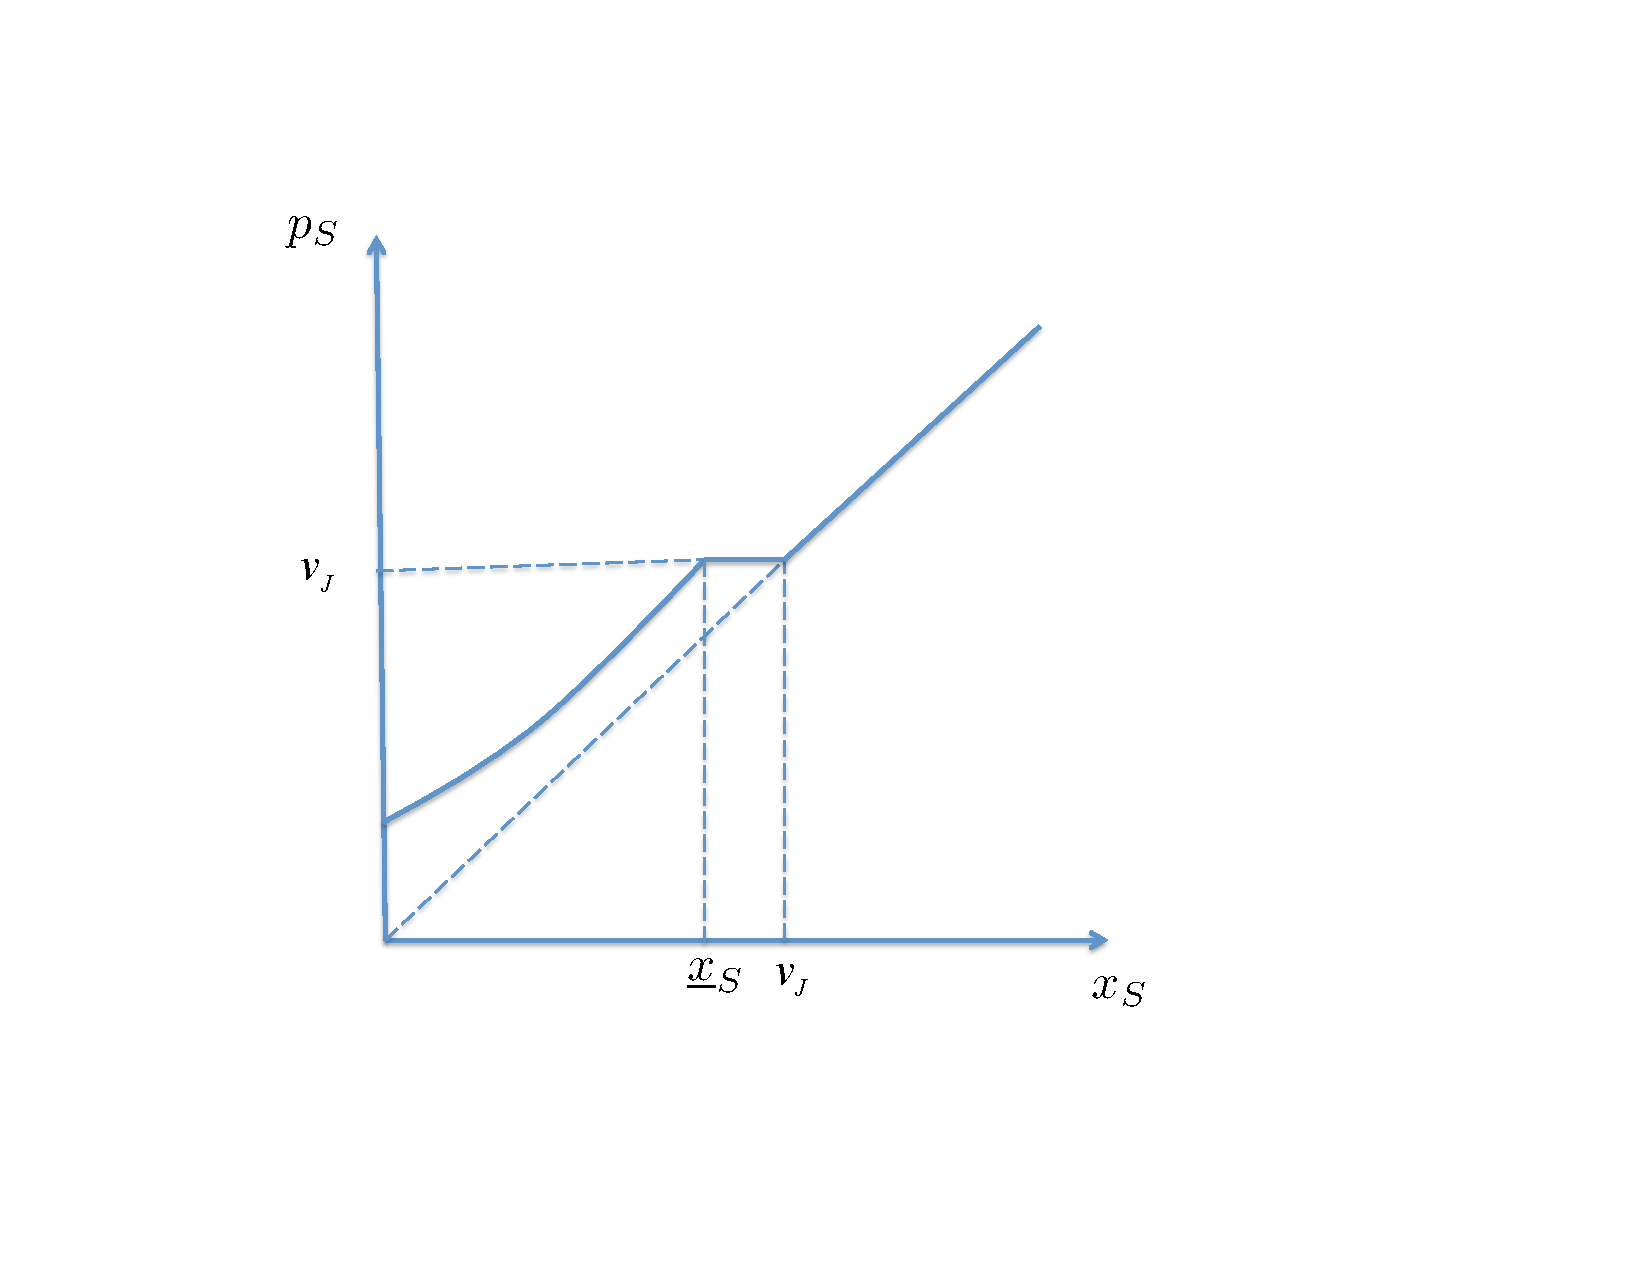
\includegraphics[scale=0.55]{graphics/equilibrium.pdf}
  \caption{Equilibrium under IPV\label{fig:equilibrium}}
\end{figure}

\begin{figure}[t]
  \centering
  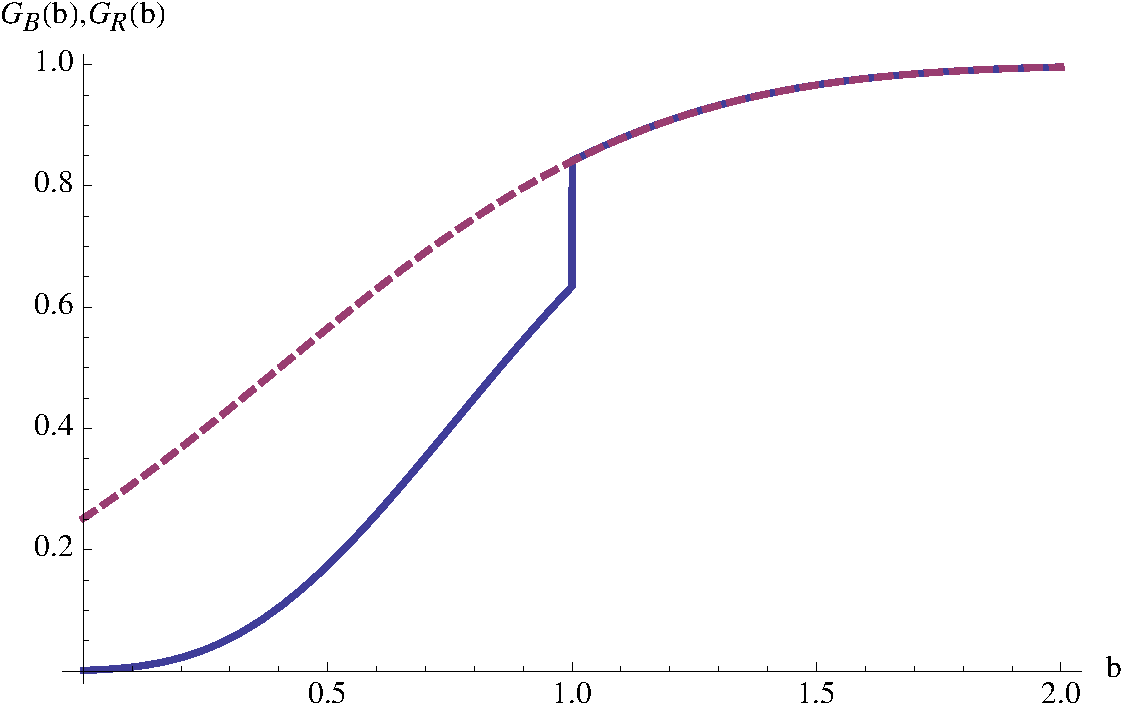
\includegraphics[scale = 0.5]{graphics/model_equilibrium}
  \caption{Computed equilibrium bid distributions for the bank
    ($G_S(\cdot)$; solid curve) and the broker ($G_B(\cdot)$; dashed
    curve). It is assumed $u_B(x_B,x_S) = x_B$, and the value
    distributions are specified as normal, with equal means $\mu_S =
    \mu_B = 0.4$ and standard deviation $\sigma_S = \sigma_R =
    0.6$. The judgment amount is $v_J=1$. Observe the mass point at
    the judgment amount in $G_S(\cdot)$.\AN{It's probably better to
      only plot the bank's bid
      distribution.}\label{fig:model_equilibrium}}
\end{figure}

\paragraph{Discussion} The bank's equilibrium behavior is different
depending on whether the bank's valuation is below or above the
judgment amount. The bank acts in a seller role in the former case,
and in a buyer role in the latter. The most interesting feature of the
equilibrium is the bunching region. In this region, the bank's dropout
prices are pooled at the judgment amount (see Figure
\ref{fig:equilibrium}).

The following intuition can be given for the bunching of banks' bids
at the judgment amount. Consider comparative statics with respect to
the banks valuation $x_S$. For low valuations $x_S$, the bank bids its
valuation plus the monopoly markup. The optimal bid of the bank
balances two effects in a trade-off: a higher bid increases the bank's
expected profits conditional on selling, but also lowers the
probability of selling the house to a third party. As we increase
$x_S$, this trade-off changes in a way that makes higher bids more
attractive to the bank. Hence, the banks bid increases with
$x_S$. However, at the point where the bank's bid reaches $v_J$, one
part of the trade-off disappears for price increase (but not
decreases): a higher bid by the bank does not increase the bank's
profit conditional on selling, since any additional revenues go to the
original owner. Therefore, as $x_S$ increases, the bank's optimal bid
stays at $v_J$. Once $x_S$ surpasses $v_J$, the bank actually prefers
retaining the property, since it is worth more than the amount
owed. Therefore, the bank's bid will again increase with $x_S$ for
$x_S$ above $v_J$.
% Why are the bank's dropout prices bunched at the judgment amount?
% To get an intuition for this, note that the bank will only benefit
% from a dropout price above $v_J$ if it keeps the house, i.e.\ wins
% the auction. Otherwise, if it sells the house, then even though the
% sale price would be higher than $v_J$, the bank stands to pocket
% only the judgment amount $v_J$. So if the bank's valuation is
% \emph{below} $v_J$, the bank would prefer to take $v_J$. This
% explains why there is a constraint $p\leq v_J$ in the bank's optimal
% pricing problem when $x_S \leq v_J$, which causes bunching at $v_J$
% for bank's values somewhat below $v_J$.
%
% This bunching will cause a \emph{mass point} at $v_J$ in the
% distribution of the bank's dropout prices.
This flat piece in the bank's bidding function corresponds to a mass
point in banks' bid distributions.  Figure~\ref{fig:model_equilibrium}
illustrates this in an example with normal distributions.

 
\section{Asymmetric information}
\label{sec:asymmetric-information}

We now consider the general environment with common values, where the
bank will be the informed party. As we shall see, there are some novel
features in this setting compared to the symmetric information
setup. The main new feature is that the equilibrium will involve a
\emph{gap} below the judgment amount. This should be intuitive since
otherwise the bank would prefer to deviate from prices slightly below
$v_J$ to offering $v_J$, leading both to a higher average price and
not changing the probability of sale.

As with symmetric information, the bank will act as a seller for lower
types, and as a buyer for higher types. Again, we begin by considering
the extreme cases $v_J = 0$, where the bank always acts as a buyer,
and $v_J = \infty$, when the bank always acts as a seller.

\subsection{Bank-buyer equilibrium ($v_J = 0$)}
\label{sec:vj0}

If $v_J=0$, both the bank and the brokers act as buyers, bidding in a
standard English auction.\footnote{We follow \cite{milgrom1982theory}
  and assume the \emph{thermometer} model, where the price is risen
  continuously from $0$ until there is only a single buyer left.} The
bank knows its valuation $x_S$, so will dropout at the price equal to
$x_S$. In a symmetric equilibrium,\footnote{By symmetric here we mean
  that the \emph{brokers} adopt the same strategy.} a broker's dropout
strategy $p_B(x_B)$ is found through the standard indifference
condition. The intuition is that, given the auction has reached price
$p$, if a broker decided to drop out at price $p$ instead to
$p+\epsilon$, this decision will change the broker's expected payoff
only if the bank (and the other brokers) dropped out at prices $p \in
(p,p+\epsilon)$. If the bank drops out at $p = x_S$, then in the limit
as $\epsilon \to 0$, the expected value of the house to the broker
will be $u_B(x_B, p)$. In equilibrium, the broker will drop out at a
price such that he is indifferent between dropping out and continuing,
while single crossing implies that brokers with higher types will
prefer to continue. Thus, a broker's type $X_B(p)$ dropping out at
price $p$ is (uniquely) found from the condition \[ u_B(X_B(p),p) =
p.\] Given our normalization $u_B(x,x) = x$, we see that $X_B(p) = p$,
so the broker, even though uninformed, in equilibrium will also drop
out at the price equal to its type. This equilibrium is described in
the proposition below.

\begin{proposition}[Bank-buyer equilibrium] 
  In a realtor-symmetric equilibrium, both the bank and the brokers
  will drop out at the prices equal to their signals, \[ p_S(x_S) =
  x_S, \quad \quad p_B(x_B) = x_B. \]
\end{proposition}

\subsection{Bank-seller equilibrium ($v_J = \infty$)}

\label{sec:comm-value-comp}




%
%
% 
% \subsection{Non-judicial foreclosures}\label{sub:nonjudicial}
%
% Recall that in a non-judicial foreclosure, the bank is entitled to
% the entire amount of the winning broker's bid. So we model a
% non-judicial foreclosure is simply an English auction where both the
% bank and the brokers are strategic participants.  This setting
% essentially involves a secret reserve price set by the informed
% seller (the bank) in a standard English auction. We will refer to
% this setting as the \emph{bank-seller equilibrium}.
Auctions in which the seller has information about the common value
component have been considered in \cite{jullien2006auction},
\cite{cai2007reserve} and \cite{lamy}.\footnote{These papers consider
  the case of a publicly observable seller's reserve price in a
  second-price auction.}  These papers consider the case of a public
reserve price and characterize a separating equilibrium in strictly
increasing, continuous and differentiable strategies.
% In the sequel, we shall refer to this equilibrium as an
% \emph{unconstrained} equilibrium.  In the foreclosure auction, the
% bank's revenue is constrained not to exceed the judgment amount.  In
% our dataset, there are some auctions with a public reserve. But in
% the majority of the auctions, the bank is an active participant. In
% other words, the bank bids just like any other bidder.
We begin by adapting the equilibrium characterization results in the
aforementioned papers to our setting.



We restrict attention to equilibria where the bank adopts an
increasing and continuous equilibrium dropout strategy $p_S^*(x_S)$,
with a differentiable inverse $X_S^*(p)$. Given our assumption that
broker signals are independent, only the bank's dropout price is
relevant for information updating. Denote a broker's dropout strategy
as $p_B^*(x_B)$, with the inverse denoted as $X_B^*(p)$. As in
\cite{milgrom1982theory}, $X_B^*(p)$ is found by equating the object's
expected value to the broker assuming the bank drops out at $p$, to
the price $p$:
\begin{align}
  u_B(X_B^*(p),X_S^*(p)) = p \label{eq:ubgen}
\end{align}
Following the bank's dropout at a price $\tilde p$, a broker's dropout
strategy is simply $u_B(x_B,X_S(\tilde p))$ as the brokers will then
have independent private values.







% In parallel to Assumption \ref{as:myerson} in the previous section,
% we assume that $J_B(x_B,x_S)$ is monotone is the buyer's
% signal.\footnote{In the independent private values (IPV) case, $
% u_B(x_B,x_S) = x_B$ according to our normalization, and one can show
% $ \frac{F_{(2)}(x_B)-F_{(1)}(x_B)}{f_{(1)}(x_B)} =
% \frac{1-F_B(x_B)}{f_B(x_B)}$. So $J_B(x_B,x_S)$ becomes the usual
% Myerson virtual value as in the previous section.}
% \begin{assumption}[Virtual value
%   monotonicity] \label{as:virtual_value} The function $J_B(x_B,x_S)$
%   is increasing in $x_B$.
% \end{assumption}
The following proposition describes the separating equilibrium in our
model.


\begin{proposition}[Bank-seller equilibrium]\label{prop:nonjudicial}
  There is a unique equilibrium in monotone differentiable
  strategies. The bank's and the broker's inverse bidding strategies
  $X_S^*(p)$ and $X_B^*(p)$ are given by the (unique) solutions to the
  differential equations
  \begin{align}
    \frac{d X_S^*(p)}{dp}&=
    \frac{(J_B(X_B^*,X_S^*)-X_S^*)]f_{(1)}(X_B^*)}{ \frac{\partial
        u_B}{\partial x_S} (u_B(X_B^*,X_S^*)-X_S^*)f_{(1)}(X_B^*)+
      \frac{ \partial u_B}{\partial x_B } \int_{X_B^*}^\infty
      \frac{ \partial u_B} {\partial x_S} f_{(2)}(x) dx
    },\label{eq:sdifeq} \\ \nonumber
    \\
    \frac{d X_B^*(p)}{dp}&= \frac{ \frac{ \partial u_B} {\partial
        x_S}( F_{(2)}(X_B^*) - F_{(1)}(X_B^*)) + \int_{X_B^*}^\infty
      \frac{ \partial u_B} {\partial x_S} f_{(2)}(x) dx }{
      \frac{\partial u_B}{\partial x_S}
      (u_B(X_B^*,X_S^*)-X_S^*)f_{(1)}(X_B^*)+ \frac{ \partial
        u_B}{\partial x_B } \int_{X_B^*}^\infty \frac{ \partial u_B}
      {\partial x_S} f_{(2)}(x) dx \label{eq:bdifeq} } ,
  \end{align}
  % \eqref{eq:sdifeq} and \eqref{eq:bdifeq},
  subject to the initial conditions $X_S^*(\ul p) = 0$ and $X_B^*(\ul
  p) = \ul p$.  The lowest price offered by the bank $\ul p$ is given
  by $ \ul p = p_S(0) = u_B(\ul x_B, 0)$, where $\ul x_B$ is the
  lowest broker type that purchases with positive probability, given
  by the unique solution to $J_B(\ul x_B,0) = 0$.  For an
  out-of-equilibrium reserve price $p<\ul p$, brokers believe that the
  bank's type is the lowest possible.
\end{proposition}
We provide the proof in the Appendix. The proof adapts
\cite{cai2007reserve} to our setting where the bank is an active
bidder in the open auction. We also show that the full-information
price is the only price that can be offered by the lowest-type bank in
such a separating equilibrium. Thus the equilibrium outcome is unique
(assuming that the strategies are differentiable and monotone). The
out-of-equilibrium beliefs for prices lower than $\underline p$ are
indeterminate, but must be sufficiently pessimistic so as to provide
the bank with an incentive not to drop out at lower prices. The most
pessimistic beliefs (i.e.\, believing that the bank's type is the
lowest possible) are reasonable, and they indeed support this unique
equilibrium outcome.



% \begin{remark}
%   \cite{cai2007reserve} obtain a parallel result for the case of a
%   public reserve. It turns out that the bank's equilibrium reserve
%   price strategy is the same as the dropout strategy above, and the
%   brokers' dropout strategy is also the same as in their paper. The
%   intuition is that $X_B(p)$, the buyer's type who drops out at
%   price $p=p_S(x_S)$ when the bank bids in the auction is the same
%   as the marginal participating buyer type at $p_S(x_S)$ when the
%   reserve price is public. So if $p_S(x_S)$ is an equilibrium bank's
%   dropout strategy in the open auction, it will also be an
%   equilibrium reserve price strategy when the reserve is public.
% \end{remark}

There is a noteworthy property of this separating equilibrium, in
comparison with the symmetric information setup considered in Section
\ref{sec:indep-priv-valu}, the \emph{signalling premium}.
\begin{corollary}[Signalling premium]\label{cor:sp}
  Under asymmetric information, the bank bids higher, $p_S^*(x_S) >
  p_S^0(x_S)$ for $x_S>0$.
\end{corollary}

\begin{proof} Our previous analysis in that section implies that the
  bank with valuation $x_S$ will set the price so that the marginal
  broker type willing to purchase at this price, $X_B^0(p)$, is found
  from the ``marginal revenue equals cost" equation
  $J_B(X_B^0(p),x_S)-x_S=0$. The price strategy itself is given by
  $p_S^0(x_S) = u_B(X_B^0(p),x_S)$. How does this price compare to the
  one with asymmetric information, $p_S^*(x_S)$? Proposition
  \ref{prop:nonjudicial} shows that there is no distortion at the
  bottom, so that the two price are equal: $p_S^*(0) = p_S^0(0)$.

  For $x_S>0$, we have $d X_S^*(p)/dp>0$. Going back the differential
  equation \eqref{eq:sdifeq}, this means that for $p=p_S^*(x_S)$, we
  must have $J_B(X_B^*(p),x_S)>x_S$, which, by the monotonicity of
  $J_B(x_B,x_S)$ in $x_B$, implies $ X_B^*(p)>X_B^0(p)$. Since
  $u_B(X_B^0(p),X_S^0(p)) = p$ and $u_B(X_B^*(p),X_S^*(p)) = p$, with
  $u_B(x_B,x_S)$ being monotone increasing in both arguments (under
  common values), we must have \[ X_S^*(p)<X_S^0(p) \implies
  p_S^*(x_S) > p_S^0(x_S)\] for $x_S>0$. \end{proof}



The signalling premium leads to welfare losses under asymmetric
information. Consider, for simplicity, the case of a single
broker. Our normalization $u_B(x_B,x_B) = x_B$ implies that it is
efficient to transfer the object from the seller with valuation $x_S$
to the buyer with valuation $x_B$ if and only if $x_B>x_S$. Denote as
$x_B(x_S)$ the minimal buyer type that will, in equilibrium, trade
with the seller with valuation $x_S$. It is found from
$u_B(x_B(x_S),x_S) = p(x_S)$. Under asymmetric information, this type
is determined from $u_B(x_B^*(x_S),x_S) = p_S^*(x_S)$, while under
symmetric information, it is determined from $u_B(x_B^0(x_S),x_S) =
p_S^0(x_S)$. Since $p_S^*(x_S)>p_S^0(x_S)$ due to the signalling
premium, we must have \[ x_B^*(x_S)>x_B^0(x_S)>x_S .\] Thus, the
trading boundary, already distorted even under symmetric information
due to the market power of the seller, is distorted even further under
asymmetric information.

Motivated by our empirical application, we now investigate how the
bank's strategy is affected as its information concerning the common
value component becomes less precise, and hence less relevant to the
brokers. Following \cite{cai2007reserve}, we consider a linear
specification in the form
\[ u_B(x_B,x_S) = x_B+\alpha x_S, \quad\quad \alpha \in [0,1).\] Here,
$\alpha$ reflects the relevance of the bank's information for the
broker.\footnote{This specification does not satisfy our normalization
  $u_B(x_B,x_B) = x_B$, but it will if we change the broker's signal
  to $\tilde x_B = \frac{x_B}{1-\alpha}$.}  As $\alpha$ decreases, the
bank's information becomes progressively less relevant to the
broker. The case $\alpha = 0$ corresponds to independent private
values. Note that this is different from the symmetric information
case considered above since now the bank's information becomes
irrelevant rather than being revealed to the brokers. We denote the
bank's strategy $p_S(x_S;\alpha)$.
\begin{proposition}[The effect of $\alpha$]\label{prop:slope}
  In the linear model, $p_S(x_S;\alpha)$ is increasing in $\alpha$.
\end{proposition}
\begin{proof}See the Appendix
\end{proof}
This result shows that, as the bank's information becomes more
relevant to the broker, the bank bids higher. In this model, $\alpha$
affects the bank's bidding incentives through two channels. First,
there is a direct channel since the bank's information directly
affects the broker's payoff. Second, there is an indirect channel due
to the signalling premium, as have discussed previously.

% In the linear model, the lowest bank's bid $p_S(0;\alpha)$ is equal
% to $J^{-\mathbbm 1} (\alpha \mathbbm E x_S) - \alpha \mathbbm E
% x_S$, and can either increase or decrease with $\alpha$ depending on
% the shape of the density $f_B(\cdot)$. If $p_S(0;\alpha)$ is
% increasing in $\alpha$, then $p_S(x_S;\alpha) <p_S(x_S;\alpha')$ for
% $\alpha<\alpha'$, i.e.\ the bank's bid increases with $\alpha$ for
% any $x_S$. But in general the monotonicity of the slope in $\alpha$
% only implies that the curves $p_S(x_S;\alpha)$ and
% $p_S(x_S;\alpha')$ cross at most once, with $p_S(x_S;\alpha')$
% crossing from below.

\subsection{General case: $v_J \in (0,\infty)$}

In a foreclosure auction with $v_J\in (0,\infty)$, the equilibrium
will combine the features of the bank-seller equilibrium for lower
$x_S$, where the bank will drop out at $p_S^*(x_S)$ as described for
the $v_J=\infty$ case, and bank-buyer equilibrium for higher $x_S$,
where the bank would drop out at $p_S^*(x_S) = x_S)$. However,
``stitching" these two equilibria under common values is by no means a
simple matter. To see the difficulties that arise, suppose we have a
bunching equilibrium with common values where the bank types over a
certain interval bid $v_J$:
\[ p_S(x_S) = v_J, \quad\quad x_S \in [\underline x_S,\overline x_S]
.\]
% Recall that in a judicial foreclosure, the bank is only entitled to
% the sale revenue up to $v_J$. As we have shown in the previous
% section, under IPV, this results in pooling of the seller's optimal
% price offers at $v_J$, while the offer below $v_J$ are unaffected.

To begin, we observe that there does not exist an equilibrium in
continuous strategies that involves bunching.
% For simplicity, consider the case when there is only one broker,
% $n=1$.  Incentive compatibility implies that the probability of
% transfer of the house to the broker must be non-increasing in the
% price $p$. As the probability of transfer is equal to
% $1-F_B(X_B(p))$, it follows that the broker's cutoff $X_B(p)$ must
% be nondecreasing.
If the bank's dropout strategy $p_S(x_S)$ were continuous and involved
bunching, then the brokers' dropout strategy $p_B(x_B)$ would involve
a gap below $v_J$, since otherwise the brokers who would contemplate
bidding slightly below $v_J$, would prefer to wait and drop out at a
price slightly above $v_J$, to take advantage of a dramatically higher
quality of the house they would be able to get for banks in the
bunching region. Such a gap in broker bids, however, creates an
incentive for the bank types that bid somewhat below $v_J$ to deviate
to the bid $v_J$, since this deviation leads to a higher expected
price, but does not change the probability of selling.

  

\begin{figure}[tf]
  \centering
  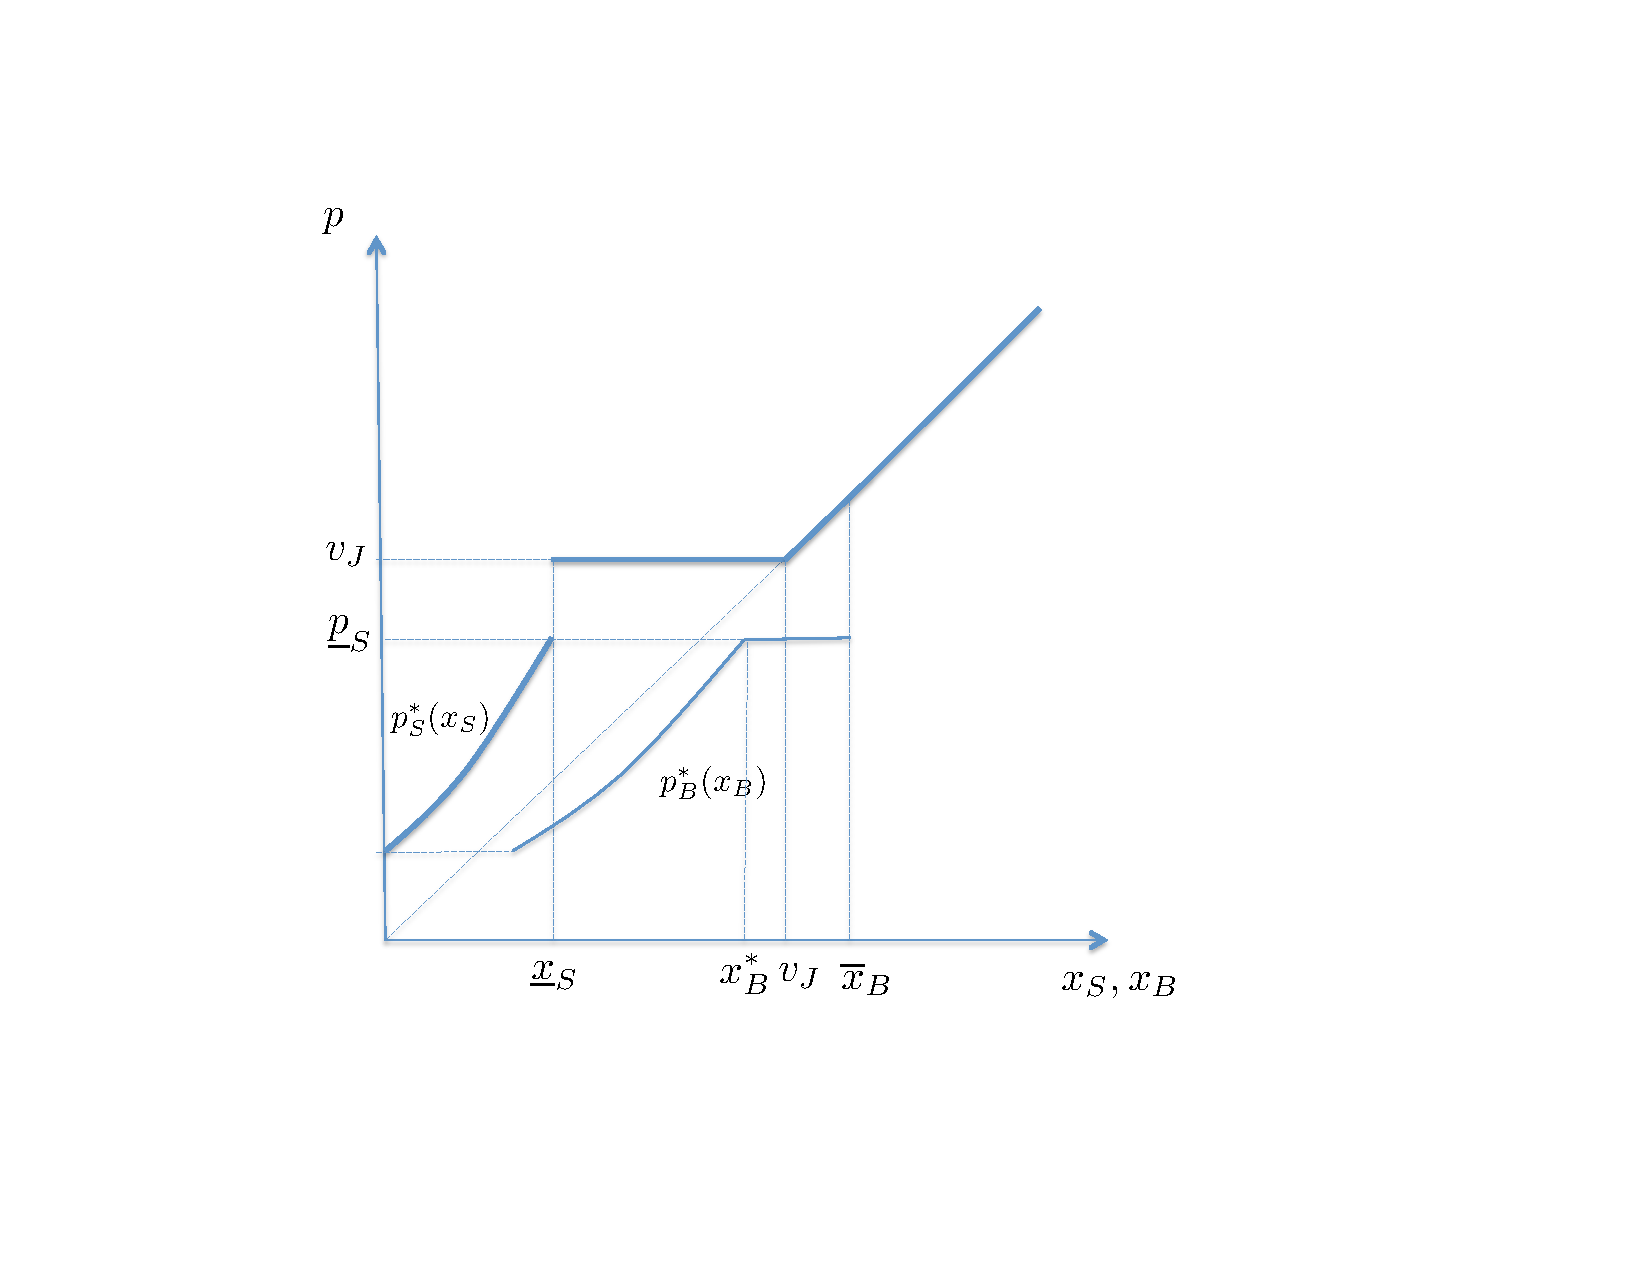
\includegraphics[scale = 0.6]{graphics/eqm_common.pdf}
  \caption{Equilibrium with common values}
  \label{fig:eqm_common}
\end{figure}

In order to prevent such deviations, an equilibrium with bunching must
involve a \emph{gap} below $v_J$, with $\underline x_S$, the seller at
the lower bound of support of the bunching region, being indifferent
between bidding $v_J$ and bidding $\ul p_S<v_J$. Sellers with
valuations slightly below $\ul x_S$ will strictly prefer bidding
slightly below $\ul p_S$ to bidding $v_J$.  The bank's strategy in our
(semi-)separating foreclosure equilibrium coincides with $p_S^*(x_S)$
derived previously for $v_J=\infty$, involves a jump at $\ul x_S$ to
$v_J$, bunching at $v_J$, and truthful bidding for $x_S > v_J$.

The broker's dropout strategy will be a best response to the bank's
strategy. It will coincide with $p_B^*(x_B)$ derived for the
$v_J=\infty$ case for $x_B < x_B^*$, where $x_B^*$ is implicitly
defined by $p_B^*(x_B^*)=\ul p_S$. Then, the types $x_B \in (x_B^*,\ol
x_B$) will drop out as soon as the price has surpassed $\ul
p_S$. These brokers realize that they cannot beat the bank profitably
at any price. The types $x_B \geq \ol x_B$ will continue, and bid up
to their values. We must have $\ol x_B > v_J$, since otherwise the
broker bidding slightly above $v_J$ would prefer a deviation to a bid
slightly above $\ul p$ in order to avoid a loss due to a lower average
quality over the bunch.

So the bank's dropout strategy $p_S(x_S)$ and the broker's dropout
strategy when the bank hasn't dropped out, $p_B(x_B)$, are given
respectively by
\begin{align}
  p_S(x_S) & =
  \begin{cases}
    p_S^*(x_S), & \quad x_S \in [0, \underline x_S], \\
    v_J,        & \quad x_S\in[\underline x_S,v_J],\\
    x_S , & \quad x_S>v_J,
  \end{cases} \nonumber \\
  p_B(x_B) & =
  \begin{cases}
    p_B^*(x_B), & \quad x_B \in [\underline x_B, x_B^*), \\
    \ul p_S,        & \quad x_B\in[x_B^*,\overline x_B] ,\\
    x_B , & \quad x_B>\overline x_B.
  \end{cases}
  \label{eq:strategies}
\end{align}
See Figure \ref{fig:eqm_common}, where the bank's and broker's bidding
strategies are shown respectively by the thick and the thin
curves.\AN{maybe change lines to dashed and solid}



We now introduce the key two conditions that will uniquely pin down
the cutoff types $\underline x_S$ and $\ol x_B$ and therefore pin down
an equilibrium.  First, the $\ol x_B$-type broker must be indifferent
between dropping out at a price slightly above $\ul p$ or staying in
up to $\ol x_B$. By deviating to a higher bid $\ol x_B$, the broker
would gain the property value $u_B(\ol x_B,x_S)$ at a price equal to
$v_J$ if $x_S \in [\underline x_S,v_J]$, and $x_S$ if $x_S \in
[v_J,\ol x_B]$. So the broker's indifference condition takes the form
\begin{align}
  0 = \int_{\underline x_S}^{\ol x_B} \Big( u_B(\ol x_B,x_S)- \max \{
  v_J , x_S \}\Big) f_S^*(x_S)d x_S =: H(\underline x_S,\ol
  x_B), \label{eq:bindif0}
\end{align}
where $f_S^*(x_S)$ is the density of the bank's types conditional on
$x_S \in [\ul x_S,\ol x_B]$,
\[ f_S^*(x_S) = \frac{f_S(x_S)}{F_S(\overline x_B)-F_S(\underline
  x_S)}.\]




The second condition specifies that the $\underline x_S$-type bank is
either indifferent between bidding $\underline p_S = p_S(\ul x_S)$ or
$p=v_J$ (if $\underline x_S > 0$), or weakly prefers the bid at $v_J$
to $\underline p_S$ (if $\underline x_S = 0$):
\begin{align}
  \Pi_S(\underline x_S,\underline p_S) &= \Pi_S(\underline
  x_S,v_J),\quad\quad & (\underline x_S > 0)
  \label{eq:sindif0}
  \\
  \Pi_S(0,\underline p_S) &\leq \Pi_S (0, v_J), \quad\quad &
  (\underline x_S = 0) \label{eq:sindif2}
\end{align}
where $\Pi_S(x_S,p)$ is the bank's expected equilibrium profit if its
type is $x_S$ and it bids $p$.\footnote{See the Appendix for the
  explicit formula for $ \Pi_S(x_S,p)$.}
% There is also a possibility of a \emph{corner solution} with
% $x_S=0$.  It corresponds to \emph{full pooling} below $v_J$, and
% only requires \[ \Pi_S(0,\underline p_S) \leq \Pi_S (0, v_J) .\]

% Note that given $\underline x_S$ and $\underline
% p_S=p_S^*(\underline x_S)$, the buyer's type that is indifferent
% between buying or not at $\underline p_S$ is uniquely determined as
% $ x_B^*$.  In this form, it is clear that \eqref{eq:sindif} is an
% equation in terms of $\underline x_S, \ol x_B$ only.  Both that,
% unlike \eqref{eq:bindif0}, this equation does not depend on
% $\gamma$.
Our first result is a technical lemma below that shows existence of
cutoffs $\underline x_S, \ol x_B$ that solve the the indifference
conditions \eqref{eq:bindif0} and \eqref{eq:sindif0}. Note that it
could happen that $\ul x_S = 0$, in which case the bunch extends all
the way to the left.
\begin{lemma}[Existence and uniqueness of the
  cutoffs]\label{lm:cutoffs}
  There exists a unique solution $(\underline x_S, \ol x_B)$ to the
  broker's and bank's indifference conditions \eqref{eq:bindif0} and
  \eqref{eq:sindif0}, \eqref{eq:sindif2}.
\end{lemma}
\begin{proof}See the Appendix.\end{proof}


Given the existence of the cutoffs, we now establish existence (and
uniqueness) of a semi-pooling equilibrium under asymmetric information
of the kind described above.
\begin{proposition}[Equilibrium
  existence]\label{prop:equilibrium_existence}
  There exists a unique equilibrium in the class of strategies given
  by \eqref{eq:strategies}.
\end{proposition}
\begin{proof}[Proof of Proposition \ref{prop:equilibrium_existence}]
  We begin with the bank's equilibrium strategy $p_S(x_S)$. The
  arguments from the previous sections imply that $p_S(x_S)$ is an
  equilibrium best response for $x_S \leq \underline x_S$ and $x_S
  \geq \overline x_B$, so in this proof we only consider $x_S \in
  (\underline x_S, \overline x_B)$. For $x_S \in (v_J, \ol x_B)$, the
  bank acts as a buyer, and it is a best response for it to bid its
  value, $x_S$.  So it only remains to consider $x_S \in (\underline
  x_S, v_J]$. These types will prefer to bid $v_J$ over any bid in
  $(\underline p_S, v_J)$. The reason is that the brokers with values
  $x_B<\overline x_B$ drop out immediately once the price has gone
  over $\underline p_S$. The brokers who remain will bid up to their
  values $x_B\geq \overline x_S$. The bank will prefer to bid $v_J$
  over any $(\underline p_S, v_J)$ since doing so will not reduce the
  probability of selling to a broker, but will at least weakly
  increase the price conditional on sale.\footnote{The price
    conditional on sale will be strictly higher $v_J>\ul p$ if there
    is only one broker who is active, i.e.\ has $x_B\geq \overline
    x_S$. If there is more than one broker, the expected price
    conditional on sale will be unchanged.}

  Having shown equilibrium incentives for the bank, we now turn to the
  broker. The results in the previous section imply that, for $x_B
  \leq x_B^*$, $p_B(x_B)$ dominates any other bid $p \leq \ul p_S =
  p_B(x_B^*)$. Since bidding $ p \in (\ul p_S,v_J) $ will not affect
  the broker's expected profit due to the fact that no other
  participant bids there, it remains to be shown that a broker with
  $x_B < \ol x_B$ will not have an incentive to deviate to a $p\geq
  v_J$. It is clear that such a broker will not have an incentive to
  deviate to a bid $p> \ol x_B$, since this would lead the broker to
  buy at prices that are too high and would result in a loss. Indeed,
  by single crossing, $u_B(x_B,p) < p$ for $p>x_B$, which implies
  $u_B(x_B,p) < p$ for $p > \ol x_B$.

  The incremental expected profit from deviation to a price $p \in
  [v_J,\ol x_B]$ is
  \begin{align*}
    \Delta \Pi_B &= \int_{\ul x_S}^{p} (u_B(x_B,x_S) - \max \{ v_J,
    x_S \}) f_S(x_S) dx_S
    \\
    &< \int_{\ul x_S}^{p} (u_B(\ol x_B,x_S) - \max \{ v_J, x_S \})
    f_S(x_S) dx_S
    \\
    &\leq \int_{\ul x_S}^{\ol x_B} (u_B(\ol x_B,x_S) - \max \{ v_J,
    x_S \}) f_S(x_S) dx_S=0
  \end{align*}
  where the first inequality follows from the fact that $u_B(x_B,x_S)$
  is increasing in $x_B$, while the second inequality follows from the
  definition of $\ol x_B$ as the type that is indifferent This shows
  that the broker with $x_B < \ol x_B$ will not have an incentive to
  deviate to a $p\geq v_J$, and it also follows that the broker types
  $x_B \in [x_B^*,\ol x_B]$ will bunch at $\ul p_S$.
%


  The equilibrium uniqueness follows because there are unique cutoff
  types $\underline x_S$ and $\overline x_S$ according to Lemma
  \ref{lm:cutoffs}.
\end{proof}






\section{Testable Hypotheses}
\label{sec:empir-pred}

Our theory predicts bunching of banks' bids at $v_J$ for both
symmetric and asymmetric information. Denoting the distribution of
bank's bids as $G_S(\cdot)$, we therefore have the following testable
hypothesis.
\begin{conjecture}[Bunching at $v_J$]\label{hyp:bunching}
  Under both symmetric and asymmetric information, the distribution
  $G_S(p)$ has an atom at $p = v_J$, formally,
  \[
  \lim_{p\uparrow v_J} G_S(p) <G_S(v_J).
  \]
\end{conjecture}

In a hypothetical world, in which the econometrician could perfectly
observe all forms of heterogeneity, it would be straightforward to
test for asymmetric information: our theory predicts a gap in banks'
bid distributions just below $v_J$ for asymmetric information
auctions, but not for symmetric information auctions. Hence, the
presence or absence of a gap could serve as a test for asymmetric
information.

However, one should not expect a gap if there is unobserved
heterogeneity with respect to information asymmetry, as one certainly
would expect in reality. If the sales of some of the houses are
characterized by asymmetric information (ASI), whereas for others the
auction is essentially under symmetric information (SI), then the SI
auction will fill out the gap. Here, by SI we mean the houses where
the bank's information is also available to the broker; in our model,
this implies that $x_S$ is observable to the broker.



But heterogeneity with respect to informational asymmetry does have
empirically testable implications.
% From now on in this section, we focus on an additive model where the
% buyer's valuation is given by
% \[ u_B(x_B,x_S) = x_B+ Take the simplest example, in which there are
% two types of houses, ``symmetric information (SI) houses" and
% ``asymmetric information (ASI) houses".
The testable implication can be derived from Corollary~\ref{cor:sp}
(the signaling premium), by observing that for ASI houses the
probability of sale is lower than for SI houses for a given bid by the
bank. The empirically testable implication stems from a selection due
to the gap for ASI auctions as described below.

For SI houses, the bank and the brokers are symmetrically informed. In
our framework, this means that the bank's information $x_S$ is
observable to the broker and that there is no gap below $v_J$. For ASI
houses, $x_S$ is not observable to the broker and there is a gap in
banks' bids in the interval $(\ul p_S,v_J)$ for $\ul p_S=p_S(\ul
x_S)$. For bank's bids below the gap for ASI houses ($p_S<\ul p_S$),
we will observe a mixture of SI and of ASI houses. The probability of
sale for such prices is the average of the high SI and the low ASI
probability of sale. In the gap ($p_S\in(\ul p,v_J)$), we only observe
high probability of sale SI houses. This selection effects leads to an
increase of the probability of sale at $\ul p_S$. For $p_S=v_J$ and
above, we again observe both SI and ASI houses, hence a downward jump
in the probability of sale at $p_S=v_J$.
%
% Then again a sharp increase of the probability of sale just above
% $p_S=v_J$, since this in the interval $(v_J,p_2)$ more weight is put
% on IPV houses since ASI houses appear only when the upper ``arm" is
% played, i.e.\ with probability $\gamma$. One should not expect a
% sharp change at $p_2$, since for $p_S>p_2$ the probability of sale
% is the same for IPV and for ASI houses. The reason that
% $1-F_{(1)}(X_B(p_S)))=1-F_{(1)}(p_S)$ is that for $p_S>p_2$, one has
% $X_S(p_S)=p_S$.
This is illustrated in Figure~\ref{fig:theory-probability-of-sale}.



In reality, one would expect that there are more than two types of
properties, that there are different degrees of asymmetric information
and hence different lower bounds $\ul p_S$ for the gaps $(\ul
p_S,v_J)$. This will smooth out the discontinuity at $\ul p_S$ in
Figure~\ref{fig:theory-probability-of-sale}, but we should still
expect that the probability of sale to increase in the bank's maximum
bid in an interval below $v_J$, and jump downwards at $v_J$. Note that
the upper bound of the gap $v_J$ is the same irrespective of the
degree of asymmetric information, hence the discontinuity at $v_J$
will not be smoothed out.  We thus arrive at the following testable
hypothesis concerning the probability of sale to the broker, denoted
as $\rho(p_S)$. We assume that the prices are normalized by $v_J$, so
that all houses have the same effective $v_J$.
\begin{figure} %[th!]
  \centering
  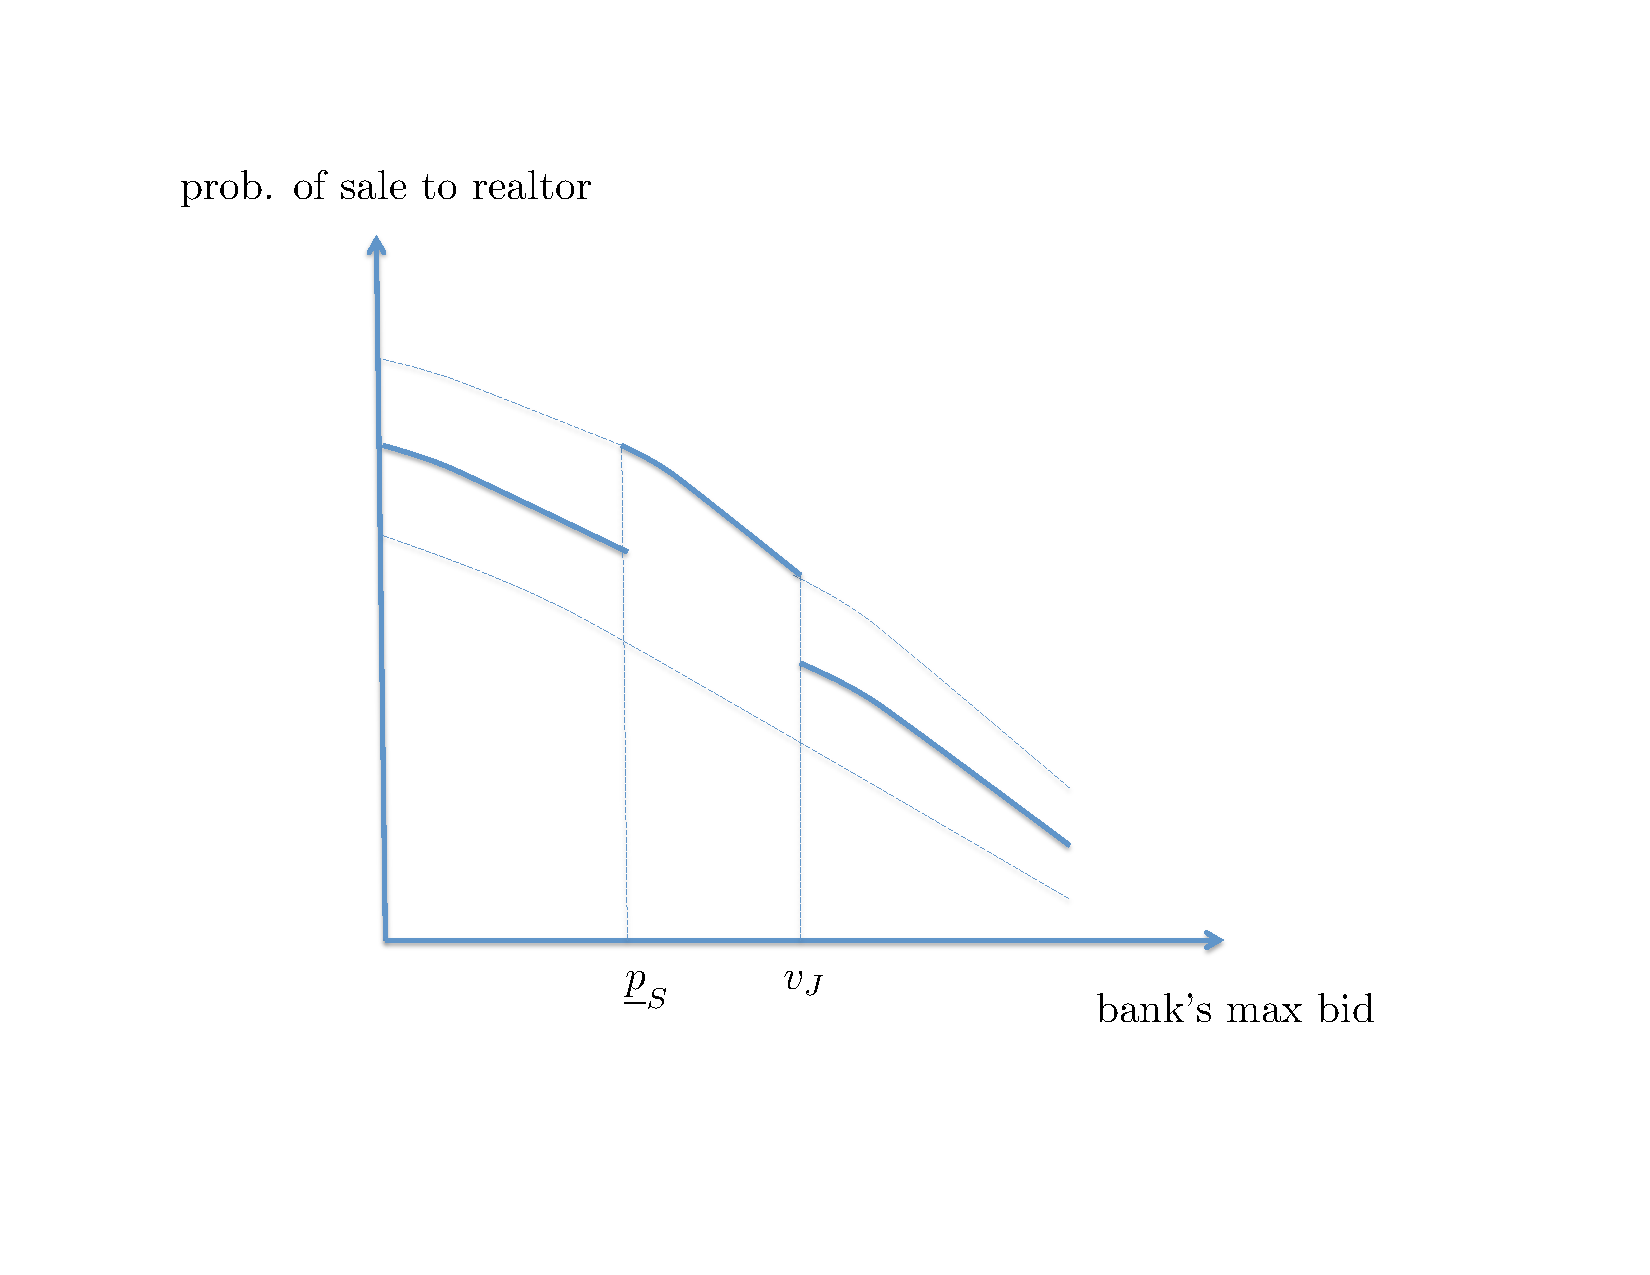
\includegraphics[scale = 0.5]{graphics/prob_of_sale}
  \caption{Probability of sale to the broker as a function of the
    bank's maximum bid for independent symmetric information houses
    (dotted, blue), adverse selection houses (red, dashed), and a
    mixture of both types of houses (black, solid).}
  \label{fig:theory-probability-of-sale}
  % \bigskip
\end{figure}
\begin{figure} %[b!]
  \centering
  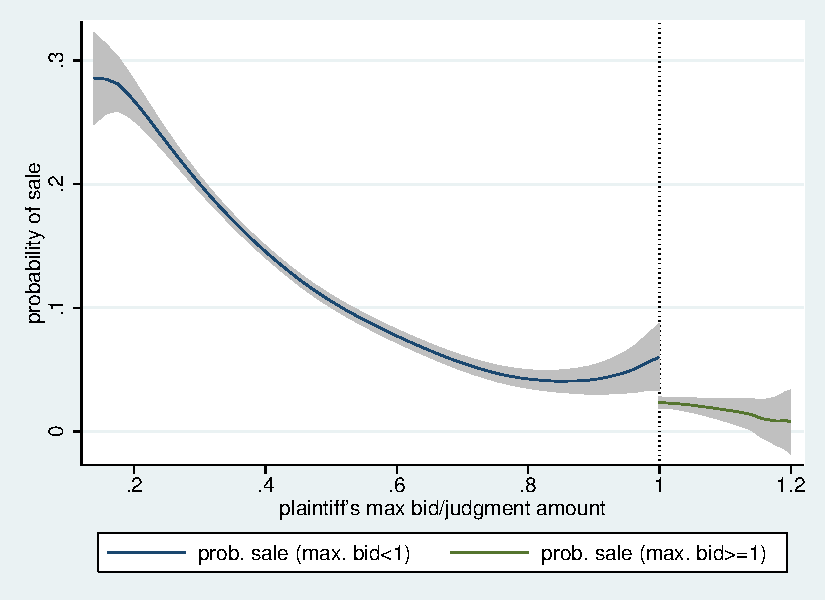
\includegraphics[scale=0.6]{graphics/simulated_simple_discontinuity}
  \caption{Simulated example for the probability of sale to the
    broker. Linear payoffs and lognormal distributions for
    $x_B,x_S$. 50,000 random draws in a Monte Carlo
    simulation. Probability of sale as a function of the bank's
    maximum bid. Locally linear kernel regression with the data split
    at $p/v_J=1$ (confidence interval: 95\%, Epanechnikov kernel and
    rule-of-thumb (ROT) bandwidth selection, see
    \cite{fan1996local}).}
%		
  \label{fig:theory-probability-of-sale_sim}
\end{figure}
\begin{conjecture}[Probability of sale]\label{hyp:discontinuity}
  If all auctions in the data are under symmetric information, the
  probability of sale $\rho(p_S)$ is a continuous, decreasing function
  of $p_S$. If, on the other hand, the data exhibit a mixture of
  auctions with a varying degree of informational asymmetry, including
  SI auctions with a positive probability, then we should expect the
  probability of sale to the broker $\rho(p_S)$ to exhibit the
  following pattern. Initially, $\rho(p_S)$ decreases in $p_S$. Then,
  over a certain interval $p_S \in [\tilde p, v_J)$, where $\tilde p <
  v_J$, $\rho(p_S)$ increases in $p_S$. At $p_S = v_J$, $\rho(p_S)$
  drops discontinuously to a lower value, $\rho(v_J)<\lim_{p_S
    \uparrow v_J} \rho(p_S)$, and from that point on, decreases in a
  continuous fashion.
\end{conjecture}
This pattern is illustrated in a simulated example in Figure
\ref{fig:theory-probability-of-sale_sim}. In this example, it is
assumed that the broker's payoff is linear in the signals,
$u_B(x_B,x_S) = (1-\beta) x_B+\beta x_S$, and the signals are
lognormally distributed. The weight $\beta$ put on the bank's
information $x_S$ is uniformly distributed on $[0,1/2]$, with $\beta =
0$ corresponding to symmetric information.



\section{Data}
\label{sec:data}

The Clerk \& Comptroller's auction website provides service for sales
on the foreclosed properties in Palm Beach county, Florida, US. The
website provides a platform for the banks (plaintiff, to whom property
owners hold liability) and potential buyers (mosty brokers), to meet
in this marketplace. The ClerkAuction online platform conducts
foreclosure sales on all business days, which provides a large amount
of data on these sales.

We collected data from the website for foreclosure sales between
January 21, 2010 and November 27, 2013. Our data record all
transaction details on these sales, including winning bid, winner
identities, and judgment
amounts.% and more importantly, the property address in the case.

% With the help of property addresses, we then resort to another
% database powered by Property Appraiser's Public Access in Palm Beach
% county. There, we collected the information regarding the properties
% being sold at the foreclosure sales. In particular, we found the
% appraisal values of property for the current year, type of property,
% and transaction value for next sale after the foreclosure sales.

% We restrict our attention with the auctions that had information on
% all the winner identity, appraisal values, and next resale values.
% In total, our data set effectively includes 2047 observations.

Our dataset contains 12,788 auctions with a total judgment amount of
\$4.2bn. The sum of winning bids is \$0.5bn.  Table \ref{sumstat}
reports the summary statistics for main variables.  The variable
\textit{bank winning} indicates that 84\% of auctions under study
ended up having properties transferred to bank's ownership.

% \begin{itemize}
% \item prob of having next sale, conditional on bank wins: 0.5673
% \item prob of having next sale, conditional on broker wins: 0.1107
% \end{itemize}

\begin{table}[!htbp]
  \centering \caption{Summary statistics \label{sumstat}}
  \begin{tabular}{lcccc}
    &&&&\\
    \hline
    \multicolumn{1}{c}{\textbf{Variable}}&\textbf{Mean}  & \textbf{Std. Dev.} 
    & \textbf{Min}& \textbf{Max} \tabularnewline
    \hline
    % bank winning &0.83	&0.38	&0	&1\\
    % number of realtors& 2.79& 1.33& 0&11\\
    bank wins & 0.813 & 0.390 & 0 & 1 \\
    number of third-party bidders & 1.065 & 1.362 & 0 & 14 \\


    &&&&\\
    \hline
    \multicolumn{1}{c}{\textbf{Variable}}&\textbf{Mean}  & \textbf{Std. Dev.} 
    & \textbf{1st Percentile}& \textbf{99th Percentile} \tabularnewline
    \hline
    \multicolumn{3}{l}{\textit{Variables with original scales}}&&\\
    % winning bid & 91868.10&	100950.02	&2300.00	&1300100.00\\
    % appraisal value & 121020.77&	138637.27&	8756.00	&2200466.00\\
    % next resale value &117989.53	&139817.89&	0.00&	2100000.00\\
    % judgment amount &317266.69&	580580.07	&4375.63	&20339327.06\\

    bank's bid & 210,996 & 1,294,181 & 4,200 & 1,476,989 \\
    judgment amount & 329,951 & 1,953,172 & 4,985 & 2,380,127 \\

    &&&&\\
    \multicolumn{3}{l}{\textit{Variables normalized by judgment amount}}&&\\
    % winning bid&
    % 0.720	&0.218	&0.202	&1.494\\
    % next resale value&
    % 0.979 &	0.494&	0.000	&8.796\\
    % judgment amount&
    % 3.746	&19.485	&0.084&	874.434\\

    bank's bid & 0.766 & 1.363 & 0.096 & 1.167 \\
    \hline
  \end{tabular}
\end{table}

We now turn to empirical tests of our hypotheses.

Hypothesis~\ref{hyp:bunching} can be easily checked by plotting the
cumulative distribution function of banks'
bids. Figure~\ref{fig:public-reserve} shows the distribution of banks'
maximum bids. Bunching shows up very clearly: there are roughly 4,000
observations bunched at the judgment amount.

% Figure~\ref{fig:bunching} shows a graph with the empirical
% cumulative distribution of bids normalized by the judgment
% amount. Observe the similarity in shape of the curves in
% Figures~\ref{fig:model_equilibrium} and \ref{fig:bunching}. In both
% there is bunching of the bank's bids at the judgment amount. Note
% that for the numerical example in Figure~\ref{fig:model_equilibrium}
% we assumed that the bank's and the realtor's distributions of
% valuations are the same, hence the overlap for bids above the
% judgment amount. However, this does not necessarily have to hold;
% indeed Figure~\ref{fig:bunching} suggests that this is not the case
% empirically.

% \begin{figure}[htbp]
%   \centering
%   \includegraphics[width=0.6
%   \textwidth]{graphics/distr-wbid-secret-1broker}%{bunching_judgement}
%   \caption{Distribution of the winning bid in auctions with a secret
%   reserve conditional on the bank losing the auction and bidding
%   against one other bidder (normalized by judgment amounts). Number
%   of observations: 478.}
%   \label{fig:bunching}
% \end{figure}

\begin{figure}[htbp]
  \centering
  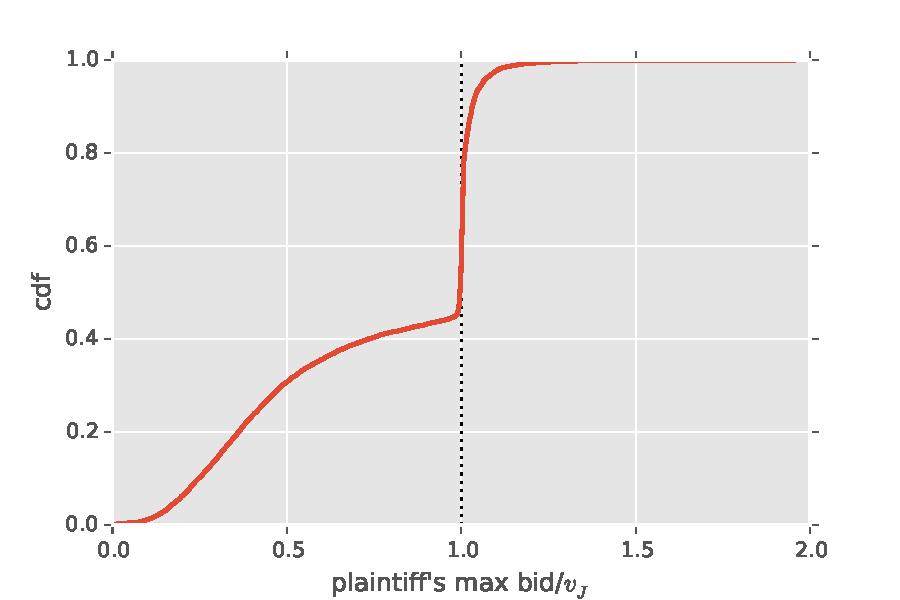
\includegraphics[width=0.6
  \textwidth]{graphics/distr-maxbid}%{bunching_judgement}
  \caption{Distribution of the bank's maximum bids (normalized by the
    judgment amounts). Number of observations: 12,788.}
  \label{fig:public-reserve}
\end{figure}


Next, we plot the probability of sale as a function of the bank's
maximum bid
(Figure~\ref{fig:discontinuity-data}). Figure~\ref{fig:discontinuity-data}
shows the same kernel regression as the one shown for the Monte Carlo
simulation in Figure~\ref{fig:theory-probability-of-sale_sim}: it is a
locally linear kernel regression, the sample being split into
observations below ($p_S<v_J$) and weakly above ($p_S\geq v_J$) the
judgment amount. The most striking feature of the graph is that the
probability of sale increases with the bank's bid just before the
judgment amount and drops down discontinuously at $v_J$.
% Figure \ref{fig:tests_nonsec} shows the estimated probability of
% sale over a band around the judgment amount, chosen as $[0,9,1.1]$,
% and over a band below the judgment amount, $[0.7,0.9]$. These bands
% are chosen sufficiently wide so that the confidence intervals around
% the estimates, also shown in the figure, are informative. It can be
% seen that the estimated probability of sale over the lower band
% ($0.093$) is smaller than the probability over the surrounding band
% ($0.159$), with the difference $0.047$. Moreover, a formal
% statistical test reveals that this difference is statistically
% significant at $5\%$ level: the t-statistic of the difference in
% means test is $2.77$.


This is exactly what theory predicts in case that there is
heterogeneity in terms of adverse selection (see
Figures~\ref{fig:theory-probability-of-sale} and
\ref{fig:theory-probability-of-sale_sim}).

% \begin{figure}[htbp]
%   \centering
%   \includegraphics[width=0.6 \textwidth]{graphics/running_smoother}
%   \caption{Probability of sale to a realtor as a function of the
%   bank's maximum drop-out price (i.e. the bank's reserve price)
%   (symmetric nearest neighbor smoothing). Dots denote individual
%   observations (at the top if the house goes to a realtor, at the
%   bottom if the bank keeps the house).}
%   \label{fig:probability-of-sale}
% \end{figure}

% \begin{figure}[htbp]
%   \centering
%   \includegraphics[scale=0.5]{tests_nonsec}
%   \caption{Probability of sale to a realtor for
%   \emph{nonsecuritized} mortgages with the bank's reserve below and
%   around the judgment amount, with confidence intervals at $95\%$
%   level.}
%   \label{fig:tests_nonsec}
% \end{figure}


\begin{figure}
  \begin{center}
    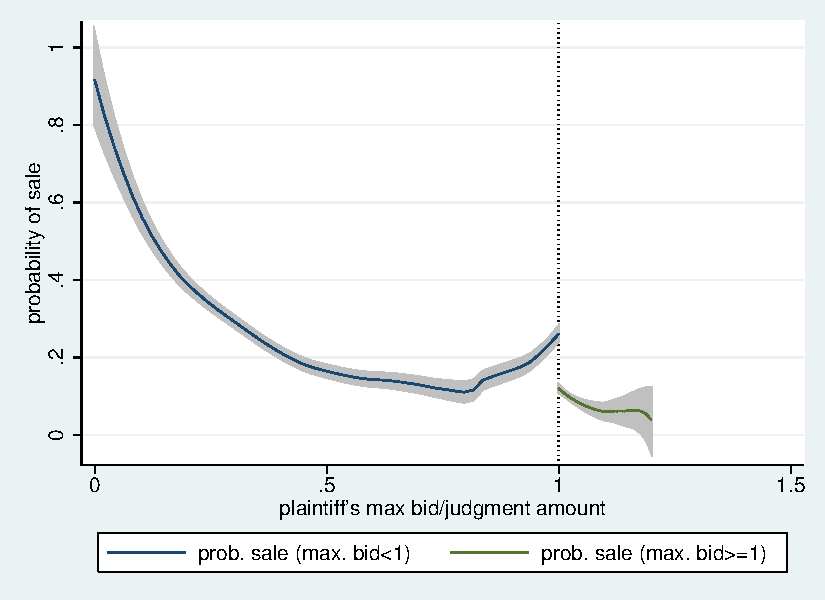
\includegraphics[width=0.6
    \textwidth]{graphics/simple_discontinuity}
    \caption{Probability of sale as a function of the bank's maximum
      bid. Locally linear kernel regression with the data split at
      $p/v_J=1$ (confidence interval: 95\%, Epanechnikov kernel and
      rule-of-thumb (ROT) bandwidth selection, see
      \cite{fan1996local}).\label{fig:discontinuity-data}}
  \end{center}
\end{figure}

% \begin{figure}
%   \begin{center}
%     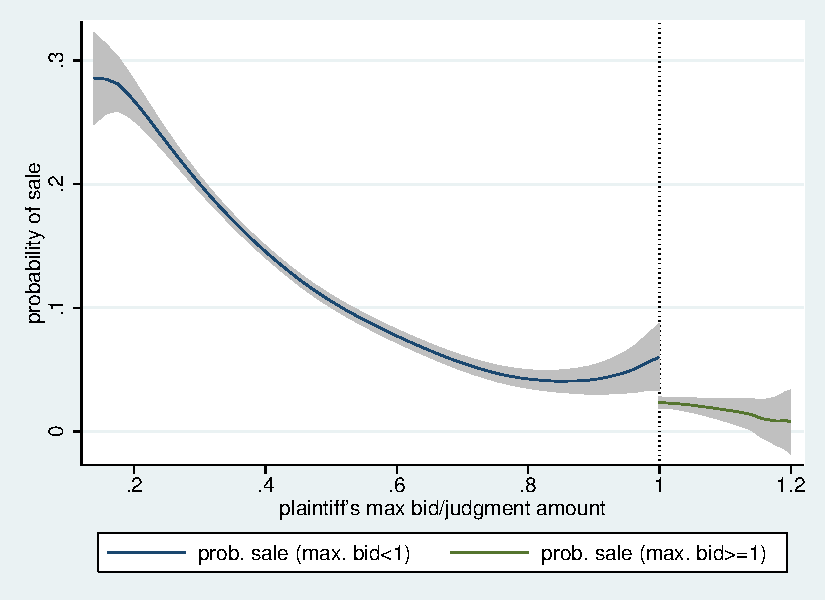
\includegraphics[width=0.6
%     \textwidth]{graphics/simulated_simple_discontinuity}
%     \caption{Estimation based on data generated by a Monte Carlo
%     simulation, using the same estimation procedure as shown in
%     Figure~\ref{fig:discontinuity-data}. Probability of sale as a
%     function of the bank's reserve price. Locally linear kernel
%     regression with the data split at $p/v_J=1$ (confidence
%     interval: 95\%, Epanechnikov kernel and rule-of-thumb (ROT)
%     bandwidth selection, see
%     \cite{fan1996local}).\label{fig:discontinuity-simulation}}
%   \end{center}
% \end{figure}

To sum up, our theory describes the effects of asymmetric information
of the seller (the bank) on the outcome of the foreclosure auction,
taking into account the judgment amount. Asymmetric information has
been recognized to be highly relevant for the understanding of how
markets works, on policy implications, and on welfare analyses at
least since Akerlof's seminal contribution on the lemon's market
\citep{akerlof1970market}. In the following section, we will describe
one important application in which asymmetric information plays a
crucial role.

% \section{Applications}
% \label{sec:applications}

\section{Securitization}
\label{sec:securitization}

% \subsection{Overview}

The securitization of mortgages massively increased before and moved
to the forefront of attention during the financial crisis. While in
1995 only 30\% of mortgages were securitized, this fraction increased
to 80\% in 2006 \cite[p. 19]{dewatripont2010balancing}. \cite{angelides2011financial} considered "collapsing
mortgage-lending standards and the mortgage securitization pipeline
[to have] lit and spread the flame of contagion and crisis" (see p. xxiii).  The
academic literature has confirmed this view and found that mortgage
securitization led to moral hazard and to banks excessively granting
mortgages, which later caused a collapse of the mortgage backed
securities market \cite{mian2009consequences,dewatripont2010balancing,keys2008did}.

Securitization involves the following steps. First, the originating
bank grants a mortgage to the home owner. Second, in order to get
liquidity, the originating bank sells the cash flows from a pool of
mortgages to a securitization agency, typically one of the Government
Sponsored Enterprises Freddie Mac or Fannie Mae. The securitization
agency splits the pool of assets into tranches and sells the tranches
to investors on the capital market. Third, if a mortgage defaults,
then the trustee of the pool of mortgages will apply for a foreclosure
at the respective court. Subsequently, the trustee of the mortgage
pool will act as the plaintiff in the foreclosure auction.

Securitization agencies have chosen measures to avoid adverse
selection. First, only mortgages can be securitized for which the
credit score (the FICO score) of the borrower is above a
threshold.\footnote{This is a somewhat simplified account, since
  securitization agencies chose two cutoffs for FICO scores: above a
  FICO score of 620, banks can securitize \emph{low documentation
    mortgages}, below a score of 600, it is very difficult to
  securitize mortgages. Between 600 and 620, banks can securitize
  mortgages, but have to provide full documentation.}  Second, the
originating bank has to offer all properties with similar observable
characteristics eligible for securitization and the agency randomly
picks the mortgages to be securitized. See \cite{keys2008did} for more
details of the securitization process.

However, securitization agencies' measures do not prevent moral
hazard, since the credit score is not a perfect signal about the
expected loss of a mortgage -- which is what the bank or the investors
buying the mortgage backed securitized ultimately care about. One
reason is that the expected loss is the product of the probability of
default and the loss given default. The credit score is only a proxy
for the probability of default, but not the loss given default. Before
the crisis, banks were known to grant mortgages with a high
loan-to-value ratio, the mortgage sometimes even exceeding the value
of the house. Since this means that only a small fraction of the
mortgage can be recovered in case of a foreclosure, this led to high
losses given default. A second reason is that the credit score is not
a perfect signal about the probability of default of a borrower. Banks
typically collect additional (soft) information to assess the
probability of default.

The securitization of mortgages reduces a bank's incentive to collect
additional information about additional components of the expected
loss (i.e. the loss given default and soft information about the
probability of default) and leads to moral hazard. \cite{keys2008did}
have shown that moral hazard led to banks collecting insufficient soft
information about the probability of default.

While the literature so far has mainly focused on the probability of
default, it is reasonable to suspect that moral hazard also led to
banks collecting insufficient information about the other component of
the expected loss, the \emph{loss given default}. This is, first,
because a high loan-to-value ratio is known to be positively
correlated both with the probability of default and the loss given
default \citep[see][and the references
therein]{qi2009loss}.\footnote{In which direction the causality goes
  is not important for our analysis. It could (and mostly likely does)
  go both ways: a high loan-to-value ratio makes strategic default
  more likely. At the same time, borrowers with financial difficulties
  are less likely to invest in the maintenance of the property, which
  decreases its value and increases the loss given default.} Second, a
more careful investigation of a potential borrower should also
directly reveal information about the value of the property.

Our theory and our data allow us to look more carefully at the
question of moral hazard with respect to the loss given default: if a
bank collected information about the value of the property (and hence
the loss given default) when it granted the mortgage, it is likely to
have an informational advantage over third-party bidders during the
foreclosure auction.

In particular, we can use information on whether a foreclosed mortgage
was securitized or not. If securitization leads to moral hazard, we
should expect the bank to have no (or only a minor) informational
advantage over third-party bidders for the case of securitized
mortgages. This means an independent private value auction (or only a
small common value component). For non-securitized mortgages we should
expect the bank to have an informational advantage. This means an
auction with a common value component on the bank's side.  This leads
us to the empirically testable implication that is an adaptation of
Hypothesis~\ref{hyp:discontinuity}:

\begin{conjecture}[Probability of sale for securitized and non-securitized mortgages]\label{hyp:discontinuity-sec-nonsec}
  For securitized mortgages, the probability of sale $\rho(p_S)$ is a
  continuous, decreasing function of $p_S$. For non-securitized
  mortgges, we should expect the probability of sale to the broker
  $\rho(p_S)$ to exhibit the following pattern. Initially, $\rho(p_S)$
  decreases in $p_S$. Then, over a certain interval $p_S \in [\tilde
  p, v_J)$, where $\tilde p < v_J$, $\rho(p_S)$ increases in $p_S$. At
  $p_S = v_J$, $\rho(p_S)$ drops discontinuously to a lower value,
  $\rho(v_J)<\lim_{p_S \uparrow v_J} \rho(p_S)$, and from that point
  on, decreases in a continuous fashion.
\end{conjecture}

% In this description of securitization, we abstracted away from a
% number of issues which are orthogonal to our analysis, but matter
% for other purposes. Some of these issues are that information may
% not be lost, but merely reduced by securitization. The FICO score,
% which is used as a threshold for securitization, is an imperfect
% measure for the probability of default. Evidence for this is
% provided by \cite{keys2008did}, who show that mortgages with a FICO
% score above the threshold were more likely to be securitized and
% also had higher probabilities of default than mortgages with FICO
% scores slightly below the threshold. Crossing the FICO score
% threshold from below increases the probability of default from 5\%
% to 5.5\%-6\%.\footnote{To be more precise, there are two thresholds
% for FICO scores. The analysis of \cite{keys2008did} mainly focuses
% on the threshold at a FICO score of 620 below which banks have to
% provide full documentation and below which banks can grant low
% documentation mortgages.} This reinforces our point that the lender
% has better information about the loss-given-default for securitized
% than for non-securitized mortgages, since the probability of default
% is known to be correlated with the loss-given-default
% \cite{qi2009loss}.
%
% Further, banks are required to keep part of the securitized
% mortgages on their balance sheets, so that banks have an incentive
% to exert less effort to collect information, not necessarily no
% effort at all. This will lead to a noisier, but not to completely
% uninformative signal for the lender in case of
% securitization. However, even with these additional issues we should
% expect the same prediction: that for a securitized mortgages the
% plaintiff is less informed than for non-securitized mortgages.

The hypothesis that the bank's information concerning the common value
component is \emph{less precise} for the securitized mortgages can
also be tested using banks' estimated bidding strategies. We do so
assuming the linear model
\[
u_B(x_B,x_S) = x_B+\alpha x_S .
\]
Proposition \ref{prop:slope} shows that the bank's strategy
$p_S(x_S;\alpha)$ is increasing in $\alpha$.  If banks holding
securitized mortgages are less informed than banks holding
non-securitized mortgages, then $\alpha$ is expected to be smaller for
the former. This leads to the following testable hypothesis.
%


\begin{conjecture}\label{hyp:slope}
  For bids below the judgment amount $v_J$, a bank holding a
  non-securitized mortgage chooses a higher bid $p^\text{nonsec}$ than
  a bank holding a securitized mortgage $p^\text{sec}$ given the same
  opportunity cost $x_S$. Formally, \[ p_S^{nonsec}(x_S) >
  p_S^{sec}(x_S), \quad\quad x_S>0 .\] \end{conjecture}

In the following, we test these hypotheses with our data.

% This is illustrated in Figure~\ref{fig:securitization}.
%
%\begin{figure}[htbp]
%  \centering
%  \includegraphics[width=0.8\textwidth]{graphics/securitization2}
%  \caption{Securitization. [Source: Gorton and Metrick
%	 (2012)]\label{fig:securitization}}
% \end{figure}

\subsection{Data}

Since we have the name of the plaintiff in each foreclosure auction,
we can categorize mortgages as securitized vs non-securitized. We use
a simple classification rule, we classify a mortgage as securitized if
the name of the plaintiff contains at least one of the following
keywords: "trust", "asset backed", "asset-backed", "certificate",
"security", "securities", "holder".\footnote{Two examples of
  plaintiff's names that are classified as securitized are "US BANK
  NATIONAL ASSOCIATION AS TRUSTEE ON BEHALF OF THE HOLDERS OF THE
  ASSET BACKED SECURITIES CORPORATION HOME EQUITY LOAN TRUST SERIES
  AEG 2006-HE1 ASSET BACKED PASS-THROUGH CERTIFICATES SERIES AEG
  2006-HE1 HSBC MORTGAGE SERVCIES INC" and "DEUTSCHE BANK NATIONAL
  TRUST COMPANY AS TRUSTEE FOR ARGENT SECURITIES INC ASSET-BACKED
  PASS-THROUGH CERTIFICATES SERIES 2006-W2".} This simple
categorization does give false negatives (for some securitized
mortgages none of the keywords shows up in the name of the plaintiff),
but almost no false positives.

We have classified 3,249 mortgages as securitized and 9,539 as
non-securitized. Figure~\ref{fig:distr-maxbid-sec-nonsec} plots the
distributions of banks' bids for securitized and non-securitized
mortgages. The average difference of the bank's bid as a fraction of
the judgment amount is much lower for securitized than for
non-securitized mortgages, roughly 40 percentage points. This could be
explained by two effects. First, a selection effect that leads to
securitized mortgages being backed by houses of lower quality. Such a
selection effect at the foreclosure auction stage can be due to moral
hazard at a previous stage, when mortgages are granted. Second, the
signaling premium leads to banks bidding higher for non-securitized
than for securitized mortgages, since the common value component plays
a larger role.

\begin{figure}
  \begin{center}
    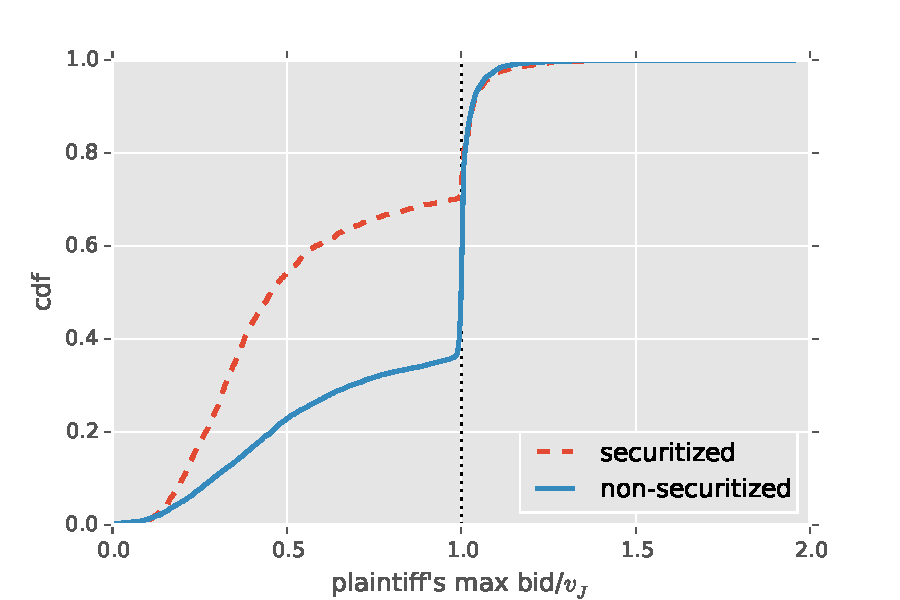
\includegraphics[width=0.7\textwidth]{graphics/distr-maxbid-sec-nonsec}
    \caption{Distribution of the bank's maximum bid as a fraction of
      the judgment amount $p_S/v_J$ for securitized (dashed line) and
      non-securitized (solid line)
      mortgages.\label{fig:distr-maxbid-sec-nonsec}}
  \end{center}
\end{figure}


% \begin{table}[!htbp]
%	\centering \caption{Descriptive statistics for securitized and
%		non-securitized mortgages.[REPORT PUBLIC RESERVE PRICES?]\label{tab:descriptive-securization}}
%	\begin{tabular}{lccc}
%		\hline\hline
%		& Proba. Sale & Sale Price/Judgment Amount Mean %& 25\% Quantile &
%		% 50\% & 75\%
%		& \# \\ \hline
%		All auctions & 16.5\% & 0.689 %& 0.242 & 0.387 & 0.953 
%		& 12,788 \\
%		Securitized & 16.8\% & 0.413 %& 0.212 & 0.307 & 0.416 
%		& 14,087 \\
%		Non-securitized: & 16.4\% & 0.827 %& 0.268 & 0.499 & 1.017 
%		& 28,928 \\
%		%  & Price & Judgment &
%		% $\frac{\text{Price}}{\text{Judgement
%		% value}}$ & \# \\
%		% & & value & &
%		% \\ \hline
%		% % All auctions & 76997 & 240964 & 0.358 & 469 \\
%		% % & (96312) & (221231) & (0.316) & \\
%		% All auctions & 76,150 & 308,740 & 0.313 & 12,788 \\
%		% & (181,014) & (1,308,201) & (1.532) & \\
%		% \hline
%		% % Securitized & 81587 & 277828 & 0.264 & 167 \\
%		% % & (93233) & (215225) & (0.181) & \\
%		% % Non-securitized & 74459 & 220579 & 0.411 & 302 \\
%		% % & (98033) & (222217) & (0.360) & \\
%		% Securitized & 87,256 & 344,098 & 0.277 & 14,087 \\
%		% & (119,882) & (990,335) & (2.505) & \\
%		% Non-securitized & 70,742 & 291,522 & 0.330 & 28,928
%		% \\
%		% & (204,047) & (1,437,471) & (0.658) & \\
%		% % Securitized, bank wins & 76589 (97714) & 273944
%		% % (231771) & 0.240 (0.153) & 129 \\
%		% % Securitized, broker wins & 98553 (74732) & 291015
%		% % (147505) & 0.345 (0.241) & 38 \\
%		% % Non-securitized, broker wins & 76958 (102873) &
%		% % 239776 (232476) & 0.311 (0.221) & 231 \\
%		% % Non-securitized, broker wins & 66331 (80405) &
%		% % 158121 (172004) & 0.736 (0.508) & 71 \\
%		\hline
%	\end{tabular}
%\end{table}

One cannot directly disentangle these two effects, hence it cannot be
seen immediately whether there is more asymmetric information for
non-securitized than for securitized mortgages. However, we can use
our theory as a tool to uncover evidence of asymmetric information. We
will take two approaches for this. The first relies on our theoretical
results on the discontinuity of the probability of sale at the
judgment amount. For the second approach, we use additional data that
we hand collected for a subset of the data set.

\subsection{Discontinuity}


Our theoretical results on the judgment amount and the effect of the
common value component help us gain more insight on asymmetric
information. Recall that in the presence of asymmetric information, we
should expect an increase and then a discontinuity in the probability
of sale as a function of the bank's bid
(Hypothesis~\ref{hyp:discontinuity-sec-nonsec}).

Figures~\ref{fig:probability-of-sale-securitized} and
\ref{fig:probability-of-sale-nonsecuritized} show the probability of
sale as a function of the bank's bid for securitized and
non-securitized mortgages. For securitized mortgages, there is no
increase in the probability of sale below the judgment
amount. Further, the discontinuity at $v_J$ is much less pronounced
and indeed not statistically significant. For non-securitized
mortgages, we still see the same pattern as in
Figure~\ref{fig:discontinuity-data}. This is consistent with the
theory that asymmetric information plays less of a role for
securitized mortgages, since the trustee of the mortgage pool is less
likely to have an informational advantage over brokers than a local
bank.

\begin{figure}[tbp]
  %	\centering
  % \includegraphics[width=\textwidth]{graphics/probability_of_sale_securitized}
	%	\caption{Probability of sale (which is equivalent to the
	% probability that the bank loses the auction) as a function
	% of the bank's public maximum bid for securitized
	% mortgages (LOWESS curve with 10\%
	% span). Only observations are taken, in which the bank's
	% maximum bid is public (bank wins in 2,671 auctions, broker
	% wins in 577 auctions). Circles denote individual
	% observations (at the
	% top if the house goes to a realtor, at the bottom if the
	% bank keeps the house).}
	%        
  \centering
  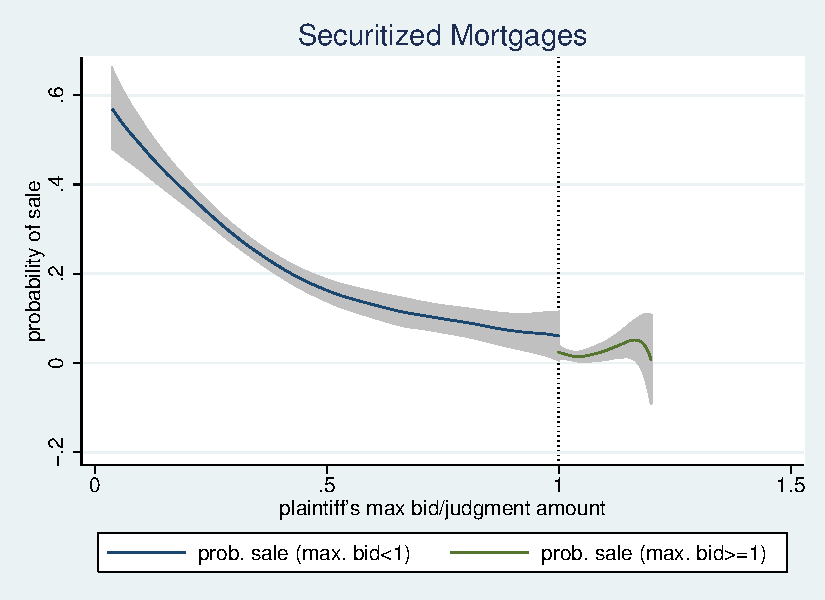
\includegraphics[width=0.6
  \textwidth]{graphics/discontinuity_securitized}
  \caption{Probability of sale as a function of the bank's maximum bid
    for securitized mortgages. Locally linear kernel regression with
    the data split at $p/v_J=1$ (confidence interval: 95\%,
    Epanechnikov kernel and rule-of-thumb (ROT) bandwidth selection,
    see \cite{fan1996local}).}
  \label{fig:probability-of-sale-securitized}
\end{figure}

\begin{figure}[tbp]
  \centering
  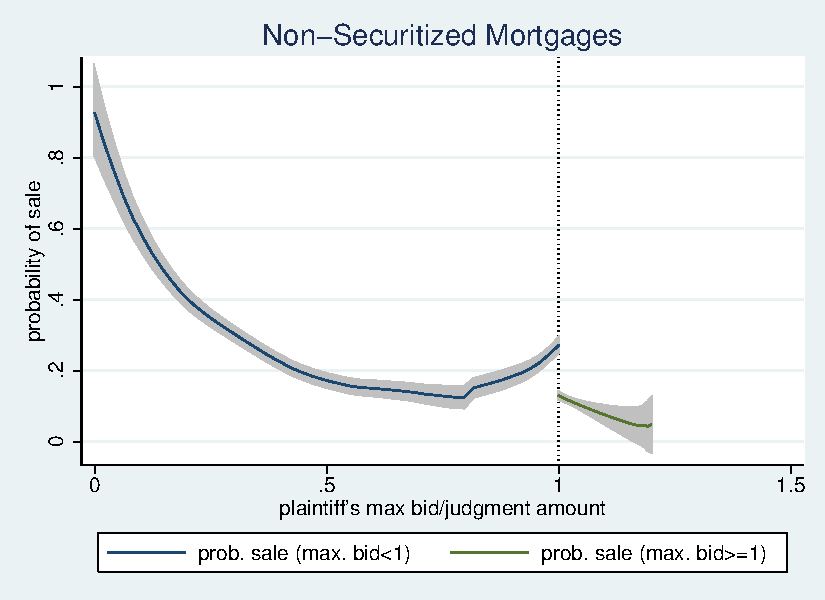
\includegraphics[width=0.6
  \textwidth]{graphics/discontinuity_nonsecuritized}
  \caption{Probability of sale as a function of the bank's maximum bid
    for non-securitized mortgages. Locally linear kernel regression
    with the data split at $p/v_J=1$ (confidence interval: 95\%,
    Epanechnikov kernel and rule-of-thumb (ROT) bandwidth selection,
    see \cite{fan1996local})}
  \label{fig:probability-of-sale-nonsecuritized}
\end{figure}


% \begin{figure}[htbp]
%   \centering
%   \includegraphics[scale=0.5]{tests_sec}
%   \caption{Probability of sale for \emph{securitized} mortgages
%   below and around the judgment amount, with confidence intervals at
%   $95\%$ level.}
%   \label{fig:tests_sec}
% \end{figure}

\subsection{Bidding Strategy}

Figures~\ref{fig:probability-of-sale-securitized} and
\ref{fig:probability-of-sale-nonsecuritized} provide indirect evidence
for a common value component for non-securitized mortgages, while
there is no such evidence for the securitized mortgages. In this
section, we develop and implement a direct test of our Hypothesis
\ref{hyp:slope},
\[ p_S^{nonsec}(x_S) > p_S^{sec}(x_S).\]

While the theoretical predictions are clear, the empirical strategy is
more involved. It is not sufficient to observe that banks' bids are
higher for non-securitized than for securitized mortgages as depicted
in Fig.~\ref{fig:distr-maxbid-sec-nonsec}. The reason for a different
distribution of bids may be either the signaling premium (higher
$p_S(x_S)$ for a given $x_S$), a selection effect (different
distributions of $x_S$ for securitized and non-securitized mortgages),
or a combination of both. We have to control for $x_S$ in order to
identify the signaling premium.


In order to be able to control for $x_S$, we have hand-collected
additional information for a subsample of our data set, namely for
properties foreclosed in September 2011. In particular, we collected
the information on property transactions after foreclosure sales from
a different data source, a website powered by the Palm Beach County
Property Appraiser (a government agent). The information regarding the
property transactions are for ad valorem tax assessment purposes, as
stated in the disclaimer of the website. This implies the appraiser
exercises auditing procedures strictly to ensure the validity of any
transaction received and posted by that office.

For each foreclosure case, we first traced back the original legal
documents, from which we found the property address. We then used the
address to search in the database for the detailed features regarding
the property and its transaction history. The property appraiser
database provides information regarding the type of property (single
family, townhouse, zero lot line, etc.), its appraisal values for the
most recent three years, the next sale date, the next sale value, and
information on the next owner. Using this information, we were able to
recover some of the next resale values of the properties at
foreclosure.

A comparison of the data on foreclosed properties and the data from
the Property Appraiser's database revealed that a perfect matching of
observations in the two data sets is not possible, since the address
listed in the legal documents is not always of the same format (or
containing the same details) as the information recorded in the
appraisal database. In order to err on the side of caution, we only
used observations for which we can be certain about the identity of
the buyer (being the property at foreclosure under study).\AN{Steven,
  I don't understand what "(being the property at foreclosure under
  study)" means. Could you please clarify.}

We identified 332 properties among 644 foreclosed cases in the
month.\footnote{There were 983 properties listed for foreclosure for
  September 2011, but 339 of them were canceled prior to the auction
  dates.} The next sale of the foreclosed properties happened mostly
in the year of 2012, though a few of the properties were not resold
until early 2013. This leaves us with 250 observations for which the
resale price is available. Since our aim is to get an estimate of the
bank's valuation distribution, we only used the data from the
foreclosure auctions in which the bank won. This restricts our sample
to 199 observations, with 77 of them in the category of securitized
mortgages and 122 cases of non-securitized mortgages.

Table~\ref{tab:descriptive-securitization-resale} provides descriptive
statistics of the data collected.\AN{[POSSIBLY ADD COLUMN WITH
  ASSESSMENT VALUE/JUDGMENT AMOUNT.]} The table suggests that part of
the difference in sales prices between securitized and non-securitized
mortgages is explained by a selection effect: the bank's resale price
in case it wins the auction is higher for non-securitized than for
securitized mortgages. In the following, we will disentangle the
selection and the signaling premium effect.

\begin{table}[!htbp]
  \centering \caption{Descriptive statistics for securitized and
    non-securitized mortgages. %\AN{[REPORT MEDIAN SALE PRICE/VJ INCLUDING OUTLIERS,
		%ASSESSMENT VALUE/VJ, QUANTILES, MENTION OUTLIERS AS REASON FOR QUANTILES]}
    \label{tab:descriptive-securitization-resale}}
  \begin{tabular}{lccc}
    \hline\hline
    & Resale Price/Judgment Amount Mean %& 25\% Quantile & 50\% & 75\% 
    & \#\\
    All auctions & 0.391 %& 0.245 & 0.359 & 0.495 
    & 199 \\
    Securitized & 0.349 %& 0.222 & 0.324 & 0.444 
    & 77 \\
    Non-securitized: & 0.417 %& 0.254 & 0.399 & 0.546 
    & 122 \\
    \hline
  \end{tabular}
\end{table}

The bank's bidding behavior is determined by its opportunity cost of
selling $x_S$, which is the expected resale price. We identify the
distribution of the unobservable $x_S$ by specifying the following
correlation structure between $x_S$, the observable resale price $r$
and the (also observable) tax assessment value $a$.
%
%
%
% Hence, $x_S$ is a noisy signal of the resale price $r$, in the
% following we will assume that it there is multiplicative
% noise. Formally,
\begin{align*}
  \tilde r & = \tilde x_S + \epsilon_r, \quad \quad \tilde a = \tilde
  x_S + \epsilon_a
\end{align*}
where $\tilde x_S:=\ln x_S-E[\ln x_S]$ is the de-meaned
log-opportunity cost of the bank, and $\tilde r$, $\tilde a$ are the
de-meaned log-resale price and tax assessment, respectively. In this
specification, the noise terms $\epsilon_r$ and $\epsilon_S$ are
mutually independent, and are also independent of $\tilde x_S$.
%
% and $\epsilon_r$ is an error term. Note that we only observe $r$,
% but not $x_S$. To identify the distribution of $x_S$, we use
% additional information about the tax assessment value of a property
% $a$. $a$ is a noisy signal about the bank's opportunity cost
% $x_S$. Assuming multiplicative noise, we can write
% \[
% \tilde a = \tilde x_S + \epsilon_a
% \]
% where $\tilde a$ is defined analogously to $\tilde x_S$.
%
% Our identifying assumption for the identification of $x_S$ is that
% $\epsilon_r$ and $\epsilon_a$ are independently distributed.
% [POSSIBLY ADD JUSTIFICATION FOR THIS. AN AVENUE WE COULD POTENTIALLY
% GO IS THAT IF $\epsilon_r$ and $\epsilon_a$ WERE NOT INDEPENDENT,
% THE BANK COULD USE THE ASSESSMENT VALUE TO UPDATE ITS ESTIMATE OF
% THE RESALE PRICE.]
Following \cite{li1998nonparametric} and
\cite{krasnokutskaya2011identification}, the underlying distribution
of $x_S$ is non-parametrically identifiable under this assumption. One
could use standard non-parametric deconvolution techniques based on
Fourier transforms to obtain the distribution of $x_S$.

However, because of sample size issues, we take a semi-parametric
approach and parametrically deconvolute the noise in the following
way.  We can identify the variance of $\tilde x_S$ by considering the
variance of different combinations of $r$ and $a$. A simple example
for this is the following set of variances and the corresponding
equations:
\begin{align*}
  \text{Var}[\tilde r] & = \sigma_r^2 + \sigma_S^2 \\
  \text{Var}[\tilde a] & = \sigma_a^2 + \sigma_S^2 \\
  \text{Var}\left[\frac{1}{2}\tilde r + \frac{1}{2}\tilde a\right] & =
  \frac{1}{4}\sigma_r^2 + \frac{1}{4}\sigma_a^2+\sigma_S^2
\end{align*}
where $\sigma_S^2$, $\sigma_r^2$, and $\sigma_a^2$ are the variances
of $\tilde x_S$, $\epsilon_r$, and $\epsilon_a$, respectively. The
above is a system of three linear equations with three unknowns
$\sigma_i^2$, $i \in \{ S,r,a \}$, and has a unique solution.

The empirical variances of $\tilde r$, $\tilde a$, and $\tilde
r/2+\tilde a/2$ will thus lead to a consistent estimate of
$\sigma_S$. Further, we use the empirical mean of $r$ as an estimate
for the mean of $x_S$, which is also consistent. We further make the
parametric assumption that $x_S$, $r$, and $a$ are log-normally
distributed. Estimates of the distributions of $x_S$ are reported in
Table~\ref{tab:xs}. The difference in means reveals that there is
indeed a selection effect: securitized mortgages have a lower resale
price to judgment amount ratio $x_S/v_J$ than non-securitized
mortgages. In the following, we will show that this selection effect
cannot explain all the difference between securitized and
non-securitized mortgages.

\begin{table}
  \begin{center}
    \begin{tabular}{l|cc||cc}
      & $\mu_S$ & $\sigma_S$ & mean & std \\
      \hline
      securitized & -1.17236 & 0.429416 & 0.33954 & 0.152791 \\
      non-securitized & -1.01577 & 0.588605 & 0.430615 & 0.277086
    \end{tabular}
    \caption{Distribution of $x_S$ for securitized and non-securitized
      mortgages. The estimate is based on a log-normal distribution
      $x_S/v_J\sim \ln N(\mu_S,\sigma_S)$.\label{tab:xs}}
  \end{center}
\end{table}


Next, observe that the distribution of banks' bids satisfies
$G_S(p_S(x_S))=F_S(x_S)$ if there is homogeneity with respect to the
common value component. Since we only observe the distribution of the
bank's resale prices if the bank wins the auction, it is useful to
define $\tilde F_S(x_S)$ and $\tilde G_S(p_S)$ the distributions of
$x_S$ and $p_S$ conditional on winning the auction.
% and
%% as $\tilde F_S(x_S):=F_S(x_S)/(1-F_{(1)}(p_S(x_S)))$. Similarly,
%% let
% $\tilde G_S(p_S):= G_S(p_S)(1-F_S(p_S))$.
Because \[ \tilde F_S(x_S) =\tilde G_S(p_S(x_S)), \]we can write
\[
p_S(x_S) = \tilde G_S^{-1}(\tilde F_S(x_S))
\]
Given that we have estimates of $\tilde G_S$ and $\tilde F_S$ both for
securitized and for non-securitized mortgages, we can estimate $p_S$
for both types of mortgages.

% Note that without unobserved heterogeneity, the function $\tilde
% G_S^{-1}(\tilde F_S(x_S))$ can be interpreted as the bidding
% function $p_S(x_S)$. With unobserved heterogeneity it should be
% interpreted as an "average bidding function". If for some
% non-securitized mortgages there is a private value auction and for
% others a common value component auction, then $\tilde
% G_S^{-1}(\tilde F_S(x_S))$ will be a weighted average of
% $p_S^*(x_S)$ and $p_S^0(x_S)$. This average would still be higher
% than the bidding function $p_S^0(x_S)$ for securitized mortgages by
% Corollary~\ref{cor:bidding-sec-nonsec}. See
% Appendix~\ref{sec:avg-bid-heterogeneity} for more details.


Figure~\ref{fig:ps-xs-sec-nonsec} shows estimates of $p_S(x_S)$ for
securitized and non-securitized mortgages. The estimates are
consistent with our Hypothesis \ref{hyp:slope}, namely that the bank's
bid is higher for non-securitized than for securitized mortgages,
controlling for the bank's opportunity cost $x_S$.

Note that comparing the bidding functions for bids below $v_J$ is
difficult, since the bidding function below $v_J$ has a different
support for securitized and non-securitized mortgages. It is more
practical to compare the inverse bidding function $x_S(p_S)$ for
securitized and non-securitized mortgages, since the support is
$[0,v_J]$ in both cases. The inverse bidding functions are shown if
Figure~\ref{fig:xs-ps-sec-nonsec}. Computing the 90\% confidence
interval of the difference of the inverse bidding functions for
securitized and non-securitized mortgages reveals that the difference
is significant for high values of $p_S$, see
Figure~\ref{fig:xs-diff-10}.
% For low values of $p_S$, the difference is not significant and close
% to 0. This is consistent with the theoretical prediction that the
% signaling premium is 0 at the lower bound of support.

\begin{figure}
  \begin{center}
    \begin{subfigure}[b]{0.5\textwidth}
      \centering
      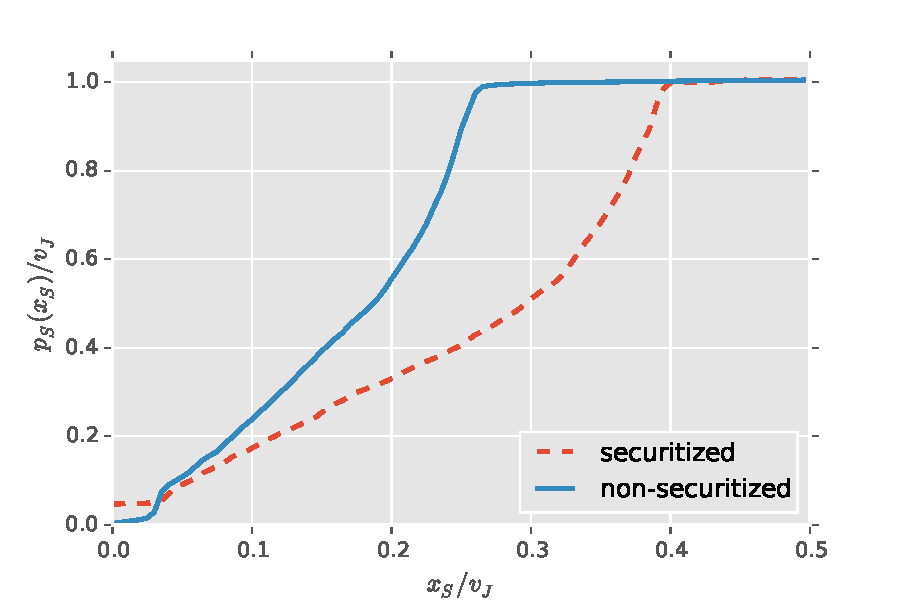
\includegraphics[width=\textwidth]{graphics/ps_xs_semiparametric}
      \caption{Bidding function\label{fig:ps-xs-sec-nonsec}}
    \end{subfigure}%
    ~%
    \begin{subfigure}[b]{0.5\textwidth}
      \centering
      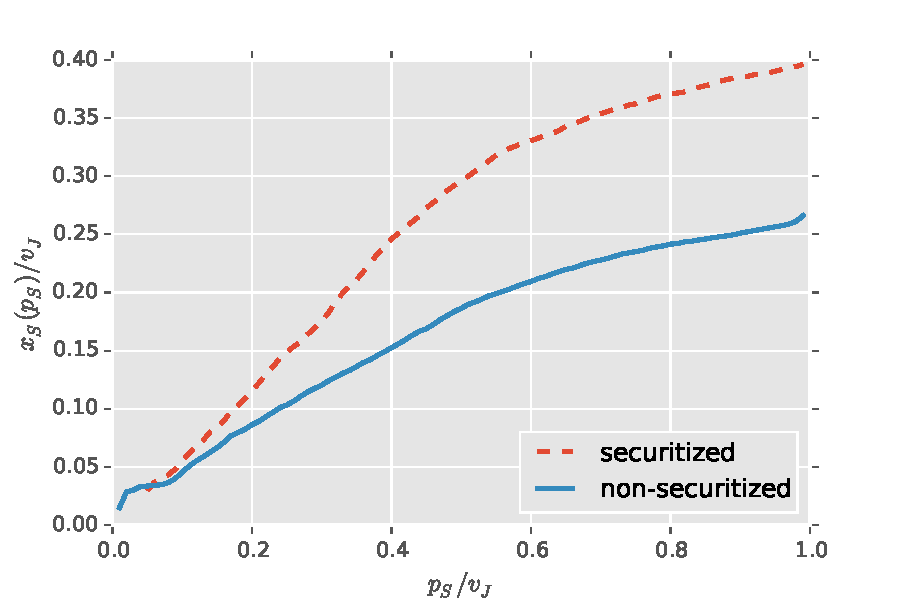
\includegraphics[width=\textwidth]{graphics/xs_ps_semiparametric}
      \caption{Inverse bidding function\label{fig:xs-ps-sec-nonsec}}
    \end{subfigure}
    \caption{Bidding function $p_S(x_S)$ and inverse bidding function
      $x_S(p_S)$ relating the bank's opportunity cost of selling $x_S$
      and the bank's bid $p_S$ for securitized (dashed line) and
      non-securitized (solid line) mortgages. The functions are
      constructed by matching quantiles of the estimated distribution
      of $x_S$ with the quantiles of observed bids submitted by
      banks.}
  \end{center}
\end{figure}

\begin{figure}[htp]
  \begin{center}
    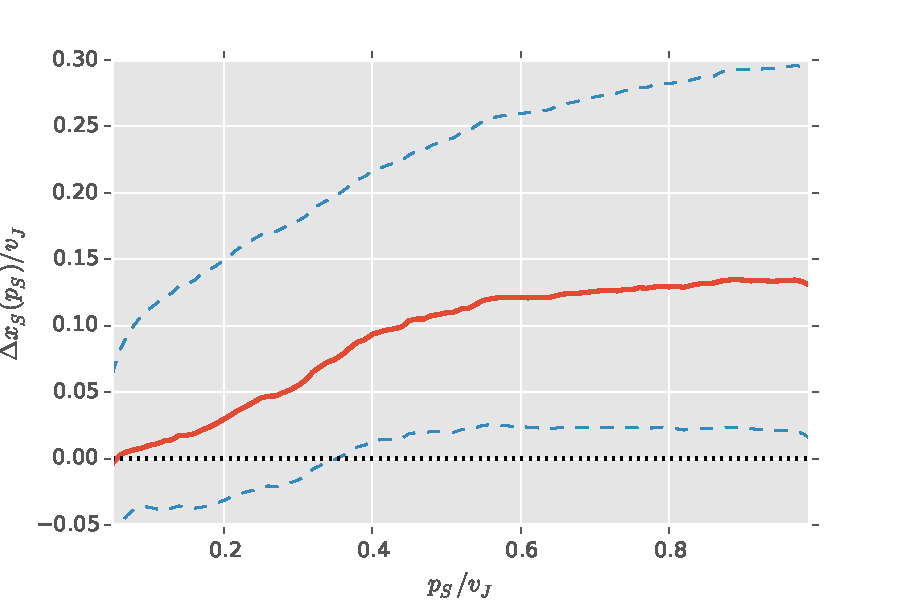
\includegraphics[width=0.7\textwidth]{graphics/xs-diff-10-line}
    \caption{Difference between banks' inverse bidding functions
      (i.e. the bank's opportunity cost of selling $x_S$ as a function
      of its bid $p_S$) for securitized and non-securitized
      mortgages. The difference (solid line) is constructed by
      matching quantiles of the estimated distribution of $x_S$ with
      quantiles of observed reserve prices submitted by banks. The 5\%
      and 95\% percentiles of the difference estimate (dashed lines)
      are constructed using a bootstrap
      estimate.\label{fig:xs-diff-10}}
  \end{center}
\end{figure}

\subsection{Implications}

The above analysis provides evidence for the existence of asymmetric
information in mortgage markets. The analysis uncovers a difference
between securitized and non-securitized mortgages and is consistent
with the hypothesis that banks holding securitized mortgages are
indeed less informed about the quality of the foreclosed property than
banks holding non-securitized mortgages.

This is consistent with the hypothesis of moral hazard in the
securitization process: if a mortgage is expected to be securitized,
then the originating bank has less incentives to collect information
about the quality of the mortgage and will be hence less informed than
for non-securitized mortgages. While the literature so far has focused
on moral hazard with respect to acquiring information about the
probability of default, our analysis has uncovered another dimension
along which there is moral hazard: The bank exerts insufficient effort
to collect information about the loss given default. Our results
suggest that the effect of securitization on the loss given default is
similarly important for the expected loss as the effect on the
probability of default. The bank's resale price as a function of the
judgment amount is 21\% lower for securitized than for non-securitized
mortgages (0.340 vs 0.431).\footnote{We provide results for the resale
  prices rather than losses given default, since there is more
  reliable data on this. A rough estimate of the difference in terms
  of the loss given default can be obtained by assuming that the loss
  given default is $v_J-x_S$. This would mean a 16\% higher loss given
  default for securitized than for non-securitized mortgages (1-0.340
  versus 1-0.431). The loss given default is typically higher than
  $v_J-x_S$, because of administrative costs.} This is comparable to
the 10\% to 20\% increase of the probability of default for
securitized versus non-securitized mortgages (5.5\% to 6\% versus 5\%)
estimated by \cite{keys2008did}.

The alternative explanation of adverse selection rather than moral
hazard in implausible because of the institutional details of the
securitization described at the beginning of this
section.\footnote{The candidate for an alternative explanation would
  be adverse selection with a pooling equilibrium, which leads to loss
  of information. For adverse selection and a separating equilibrium,
  no information is lost.} In particular, the securitization agency
prevent originating banks from cherry picking the mortgages they want
to securitize and randomly selects mortgages from a mortgage pool. See
\cite{keys2008did} for more details.

Another alternative explanation is that originating banks do collect
information about the loss given default, but this information is lost
at a later stage. However, this is also implausible, because
originating banks are required to hold tranches of the securitized
mortgage pool. If they had any relevant information about the quality
of the property, they would have an incentive to use it in the
foreclosure auction (or to share it with the plaintiff in the
foreclosure auction).

Our results have a number of policy implications. First, it provides
further support for the concern about moral hazard in the
securitization process. Our findings hence speak in favor of policies
seeking to reduce moral hazard, such as requiring better documentation
for securitized mortgages, reducing government support for
securitization through securitization agencies, or holding the
originating bank liable in case a mortgagee defaults (as is the case
for European covered bonds), see e.g. \cite{keys2008did},
\cite{tirole2011illiquidity}, and \cite{campbell2013mortgage}.

Second, our results emphasize an additional dimension besides the
probability of default along which moral hazard can affect the
securitization process: the loss given default. This suggests that
documentation not just of the characteristics of the borrower, but
also of the property are important. At the same time, our finding also
highlights some of the difficulties in new regulations: new regulatory
requirements set criteria for the documented loan-to-value ratio of
mortgages, e.g. the new Solvency II Directive of the European Union
requires that mortgages in the securitization pool to meet certain
requirements on the loan-to-value ratio\footnote{See the Commission
  Delegated Regulation (EU) 2015/35, Article 177(1)(h).} However, our
results suggest that there is asymmetric information about the value
of properties and hence also about the loan-to-value ratio.

% \subsection{Non-Judicial Foreclosures}
% \label{sec:non-judic-forecl}
%
% In this paper we have developed a theory of judicial foreclosures,
% i.e. foreclosures that are organized by a court. Roughly half of the
% states in the U.S. (including Florida) only allow judicial
% foreclosures. The other half of the states allow both judicial and
% non-judicial foreclosures. In a non-judicial foreclosure, the lender
% typically has the \emph{power of sale} and can seize and sell the
% house without going through a court. In the law literature on
% foreclosure reform, it has been argued that allowing the bank to
% seize the property and actively marketing it would simplify the
% sales process \cite{nelson2004reforming}. It would also make it
% easier for realtors to inspect the property, thereby reducing --
% even if not completely removing -- asymmetric information. In the
% following, we show the relevance of different foreclosure
% procedures. To make the discussion simple, we take the extreme
% stance that a non-judicial foreclosure allows to completely remove
% the asymmetric information. In practice, one would expect that
% asymmetric information would be reduced rather than completely
% removed.\footnote{In practice, the non-judicial foreclosure
% procedure is also less extreme than described here. Only Delaware
% \citep{ghent2011recourse} has the extreme case of strict
% non-judicial foreclosures in which all proceedings of the sale go to
% the bank and the original owner gets nothing. Other states with
% non-judicial foreclosures have limited borrower protection, see
% \cite{ghent2011recourse}.}
%
% Note that comparing the utility of the original owner would be
% trivial: with non-judicial foreclosures, the original owner does not
% get anything, whereas with a judicial foreclosure, he may get
% something, so he is trivially better off.
%
% Therefore, instead of the original owner's utility, we will compare
% overall welfare in judicial and non-judicial foreclosures. Note that
% we only need to consider the allocation rule, since transfers do not
% matter for welfare. An allocation rule consists of the probability
% $Q_S(\boldsymbol x_B,x_S)$ that the seller gets the house and the
% probability $Q_B^i(\boldsymbol x_B,x_S)$ that buyer $i$ gets the
% house as a function of the seller's signal $x_S$ and the vector of
% buyers' signals $\boldsymbol x_B=(x_B^i)_{i=1}^n$. Welfare is then
% the expected sum of utilities for a given allocation rule:
% \begin{equation}
%	\label{eq:welfare}
%	\int_0^\infty ... \int_0^\infty \left[\sum_{i=1}^n Q_B^i(\boldsymbol
%	x_B,x_S) u_B(x_B^i,x_S)+Q_S(\boldsymbol x_B,x_S) u_S(x_S)\right]
%	dF_B(x_B^1)...dF_B(x_B^n)dF_S(x_S)
%\end{equation}
%Observe that $u_B(x_B,x_S)>u_S(x_S)$ iff $x_B>x_S$ since $u_B(x,x)=x$
% and $u_B$ and $u_S$ are weakly increasing in their
% arguments. Therefore, the social planner would maximize
% \eqref{eq:welfare} by giving the house to the bidder with the
% highest signal $x$. Formally, the first-best allocation rule is
% \[
% Q_S^*(\boldsymbol x_B,x_S) =
% \begin{cases}
%   1 & \text{if $x_S>\max_i x_B^i$,} \\
%   0 & \text{otherwise,}
% \end{cases}
% \]
% and
% \[
% Q_B^{i*}(\boldsymbol x_B,x_S) =
% \begin{cases}
%   1 & \text{if $Q_S^*(\boldsymbol x_B,x_S)=0$ and $x_B^i>x_B^j$ for all $j\neq i$,} \\
%   0 & \text{otherwise.}
% \end{cases}
% \]
% As usual, an arbitrary tie-breaking rule can be specified for the
% zero-probability event that two signals are exactly the same.
%
% For a non-judicial foreclosure auction, we assume that the bank
% sells the house in a standard auction with the same buyers with the
% same valuations showing up as in a judicial foreclosure
% auction. However, the bank is able to transmit the information to
% the realtors directly, by advertising the property and allowing
% inspections. Thus the nonjudicial foreclosures will be described by
% independent private values model, with $x_S$ directly revealed to
% the realtors.
%
%\paragraph{Independent Private Values}
%In an independent private values setup, the bank sets the reserve
% price equal to $J_B^{-1}(x_S)$ for all values of $x_S$ in a
% non-judicial foreclosure where the virtual valuation function is
% defined as $J_B(x_B):=x_B-(1-F_B(x_B))/f_B(x_B)$. Thus the marginal
% buyer's cutoff is also equal to $J_B^{-1}(x_S)$. In a judicial
% foreclosure, the marginal buyer type is given by $J_B^{-1}(x_S)$ for
% $x_S<J_B(v_J)$ and is equal to $x_S$ for $x_S>v_J$.
%
% Figure~\ref{fig:judicial-ipv} shows the boundaries of the different
% allocation rules for the one buyer case.  In first-best the buyer
% gets the house, if the realization of signals is above the 45 degree
% line (dashed). For judicial foreclosures, the buyer gets the house
% above the dotted blue line. For non-judicial foreclosure, the buyer
% gets the house above the sold red line. It is straightforward to
% show that welfare is higher with judicial foreclosures than with
% non-judicial foreclosures, since the deadweight loss of monopoly
% (the area between the dashed and solid line for judicial, the area
% between the dashed and the dotted line for non-judicial
% foreclosures) is smaller.
%
%\begin{figure}[tbp]
%  \centering
%  \includegraphics[width=0.5\textwidth]{graphics/judicial-ipv}
%  \caption{Judicial versus non-judicial foreclosure with independent
%	 private values. Lines separating the regions in which the
%	 seller and in which the buyer gets the house for first-best
%	 allocation (black dashed 45 degree line), for judicial
%	 foreclosure (solid red), and non-judicial foreclosure (blue
%	 dotted).}
%  \label{fig:judicial-ipv}
%\end{figure}
%
%\paragraph{Common Values}
%With adverse selection, the situation is more complicated as
% illustrated in Figure~\ref{fig:judicial-common-values} for the one
% buyer case. The blue dotted line corresponds to the non-judicial
% foreclosure and comes from the solution under private values, where
% the realtor knows $x_S$. The marginal buyer type with whom the
% $x_S$-type bank will trade is found at the solution to the
% ``marginal revenue equals cost" equation, \[
% J_B(x_B^{nonjud}(x_S),x_S) = x_S.\] The red solid line is the
% allocation rule for the judicial foreclosure implied by the seller's
% pricing behavior derived in our paper, i.e. $X_B(p_S(x_S))$. Observe
% that, due to the signalling premium, the solid line is above the
% dotted line for $x_S<x_B^2$. However, since the judicial auction is
% fully efficient for $x_S>x_B^2$, the solid line is below the dotted
% line for $x_S>x_B^2$. Hence, it is ambiguous whether welfare would
% be larger or smaller for non-judicial foreclosures.
% \begin{figure}[tbp]
%   \centering
%   \includegraphics[width=0.5\textwidth]{graphics/judicial-common-values1}
%   \caption{Judicial versus non-judicial foreclosure with a common
%   value component. Lines separating the regions in which the seller
%   and in which the buyer gets the house for first-best allocation
%   (blue dotted 45 degree line), for judicial foreclosure (solid
%   red), and non-judicial foreclosure (blue dashed).}
%   \label{fig:judicial-common-values}
% \end{figure}
%
% One gets a clear-cut welfare comparison if one lets $v_J$ go to
% infinity. In this case, the reserve price set in a non-judicial
% foreclosure auction $p_S^0(x_S)$ is lower than the price set in a
% judicial foreclosure $p_S^*(x_S)$ due to the signaling
% premium. Since $p_S^*(x_S) > p_S^0(x_S) > x_S$ and the first-best
% reserve price is $x_S$, non-judicial foreclosures are more welfare
% efficient.
%
% While a welfare ranking of judicial versus non-judicial foreclosures
% depends on market conditions, our results do suggest some welfare
% comparisons. For instance, for securitized mortgages, judicial
% foreclosures are likely to be more efficient than non-judicial
% foreclosures, since the relevance of the common value component
% seems to be relatively small.
%
% On the other hand, in times of financial distress, when many
% mortgages are "under water", the price is usually low compared to
% the judgment amount. Hence, $v_J\rightarrow\infty$ is a reasonable
% approximation and non-judicial foreclosures are more efficient.
%
\section{Conclusions}

We develop a novel theory of foreclosure auctions and test some of its
predictions with data from Palm Beach county (Florida, US). We find
evidence for strategic bidding and asymmetric information, with the
bank being the informed party. First, the data reveal bunching in bids
at the judgment amount as the theory predicts either under symmetric
or asymmetric information. Second, there is a discontinuity in the
probability of sale to the brokers, as the theory predicts under
asymmetric information. Third, by looking separately at securitized
and non-securitized mortgages, we find that banks bid lower for the
securitized mortgages. Our theory predicts lower bids when the bank is
less informed.

The latter findings are consistent with the hypothesis that moral
hazard is involved in the securitization process: banks expect not to
suffer from the entire loss of a default of a borrower. Hence, they
will exert less effort collecting information about the value of the
property used as collateral for a mortgage. These findings complement
the findings in \cite{keys2008did} that banks collect less information
about the probability of default for securitized than for
non-securitized mortgages.

% Recent literature, e.g.\ \cite{keys2008did} has emphasized the role
% of soft information as the predictor of the probability of default.
% Only hard, verifiable information is priced when the mortgage is
% securitized. Knowing that the mortgage will be securitized, the
% lender may not have sufficient incentives to collect soft
% information. On the other hand, \cite{qi2009loss} present evidence
% that the probability of default and loss given default are
% positively correlated. Thus, soft financial information is relevant
% for the property resale values, and loss of this information for the
% securitized mortgages means also less information about the resale
% values, thereby leading to lower bids in the foreclosure auctions.
%
% The implication of our findings in terms of the policy debate about
% securitization is that there is an additional reason to be cautious
% about securitization. This speaks in favor of some of the policies
% that have been proposed, such as requiring better documentation for
% securitized mortgages, reducing government support for
% securitization through securitization agencies, or holding the
% originating bank liable in case a mortgagee defaults (as is the case
% for European covered bonds), see e.g. \cite{keys2008did},
% \cite{tirole2011illiquidity}, and \cite{campbell2013mortgage}.

%
% which implies that our finding is consistent with the moral hazard
% story.
%
%
% To the extent that such information is correlated with the value of
% the house, our results are consistent with the moral hazard
% explanation.
%
% Our theory has the following main empirically testable predictions:
% (i) that banks' bids are bunched at the judgment amount, (ii) if
% there are both independent private values and common value component
% auctions, there will a non-monotonicity and discontinuity of the
% probability of sale in the bank's bid (the probability of sale
% increases with the bank's bid just below and drops down at the
% judgment amount). Using a novel data set, we show that predictions
% (i) and (iii), but not (ii) are consistent with the data. This can
% be interpreted as both independent private values and common value
% component auctions showing up in the data set. Further, the data are
% consistent with the claim that adverse selection plays less of a
% role for securitized than for non-securitized mortgages. This is
% consistent with the idea that local banks with non-securitized
% mortgages have better information about the common value component
% than non-local banks who act as trustees for pools of securitized
% mortgages. These findings speak in support of policy proposals that
% seek to restrict securitization.

Our theory can also be used for a welfare comparison of judicial and
non-judicial foreclosures.
% Besides securitization as an application of our theory, we provide a
% second example of an application: the welfare comparison of judicial
% and non-judicial foreclosures.
According to \cite{nelson2004reforming}, roughly $40\%$ of the states
in the U.S. (including Florida) only allow judicial foreclosures,
i.e. the foreclosure auction has to be run by a court with rules as
the ones described in this article. The other half of the states allow
for both judicial and non-judicial foreclosures.  Mortgage contracts
with a so called a ``power of sale'' clause allow the bank to choose a
non-judicial foreclosure in case of a failure to repay, i.e. the bank
can directly seize the property and sell it without going through a
court.

The power of sale clause allows the bank to market the property, and
to verifiably disclose, through inspections, some of the information
regarding its condition. This reduces the signalling premium, but
introduces another distortion. The bank, acting as a de facto owner of
the property, is no longer obligated to pay the owner back any auction
proceedings above the judgment amount. Thus the monopoly price
distortion now extends to prices above the judgment amount. So the
overall welfare effect of the power of sale is ambiguous. We plan to
estimate this effect in future work.

\bibliography{foreclosures}
% \bibliography{bilateral} \bibliographystyle{econometrica}
% \bibliographystyle{plainnat}
\bibliographystyle{ecta}
\appendix
\section*{Appendix}
\section{Omitted Proofs}
\begin{proof}[Proof of Proposition \ref{prop:nonjudicial}]
  For the exposition, we assume $n \geq 2$. The proof for $n=1$ is
  parallel. It turns out convenient to restate the problem a bit
  differently. Consider the bank of type $x_S$ that contemplates a
  dropout price $p$, and assume that the brokers hold the belief $\hat
  x_S$ concerning the bank's type following the bank's dropout. For
  now, this belief is not necessarily the equilibrium belief.
  % The broker's dropout strategy is then given by $u_B(x_B, \hat
  % x_S)$ and the broker's cutoff $\hat X_B(p)$ is determined from the
  % indifference condition \[ u_B(\hat X_B(p),\hat x_S) = p .\]

  We restrict attention to equilibria where the broker's dropout
  strategy (if the bank has not dropped out) is a continuous, strictly
  increasing function, with a differentiable inverse $X_B^*(p)$. Then
  the bank's expected profit, as a function of own type $x_S$, the
  perceived type $\hat x_S$, and the price $p$ is given by
  \begin{align}
    \hat \Pi(x_S,\hat x_S,p) &= p (F_{(2)}(X_B^*(p)) - F_{(1)}(X_B^*(p)))\nonumber\\
    &+\int_{ X_B^*(p)}^{\infty} u_B(x,\hat x_S) f_{(2)}(x)dx +x_S
    F_{(1)}(X_B^*(p)).
    \label{eq:PiS}
  \end{align}
  % Here, we provisionally assume that the broker's dropout strategy
  % is a continuous, strictly increasing function, with a
  % differentiable inverse. This implies that the broker types with
  % $x_B > X_B (p)$ will prefer to continue bidding, while the types
  % $x_B < \hat X_B(p)$ will drop out earlier.
  A direct calculation shows that
  \begin{align} \frac{\partial \hat \Pi_S}{\partial p} &=
    (p-u_B(X_B^*(p),\hat x_S)) f_{(2)}(X_B^*(p))X_B^{*'}(p) \nonumber
    \\
    &+(x_S - p) f_{(1)}(X_B^*(p))X_B^{*'}(p) \nonumber
    \\
    &+F_{(2)}(X_B^*(p)) - F_{(1)}(X_B^*(p))
    % -n f_B(\hat X_B(p))F_B(\hat X_B(p))^{n-1} \Big( J_B(\hat
    % X_B(p),\hat x_S) - x_S \Big) \hat X_B'(p)
    \label{eq:sp}
  \end{align}
  and
  \begin{align} \frac{\partial \hat \Pi_S}{\partial \hat x_S} =
    \int_{\hat X_B(p)}^{\infty} \frac{\partial u_B(x,\hat
      x_S)}{\partial \hat x_S} f_{(2)}(x)dx .\end{align}


  The bank's expected profit following a deviation from the
  equilibrium price to some other price $\hat{p}$ is equal to $\hat
  \Pi_{S}(x_{S},X_{S}(\hat{p}),\hat{p})$.  In equilibrium, such a
  deviation should not be profitable,so that the following first-order
  condition (FOC) must hold for $p\in(\underline{p},\infty)$:
  \[
  \frac{\partial \hat \Pi_{S}(x_{S},X_{S}(p),p)}{\partial p}=0.
  \]
  Substituting into this FOC the bank's type that bids $p$,
  $x_{S}=X_{S}^*(p)$, we obtain the following differential equation:
  \begin{align}
    \frac{d X_{S}^*(p)}{dp} & =-\frac{\partial\hat
      \Pi_{S}(X_{S}^*(p),X_{S}^*(p),p)/\partial
      p}{\partial\Pi_{S}(X_{S}^*(p),X_{S}^*(p),p)/\partial\hat{x}_{S}}
    % \\
    % &=\frac{-n f_B(X_B^*(p))F_B(X_B^*(p))^{n-1} \Big(
    % J_B(X_B^*(p),X_S^*(p)) - X_S(p) \Big)} {\int_{\hat
    % X_B(p)}^{\infty} \frac{\partial u_B(x,X_S^*(p))}{\partial \hat
    % x_S} f_{(2)}(x)dx} \frac{dX_B^*(p)}{dp}
    \label{eq:ivp}
  \end{align}

  We now turn to the broker's equilibrium dropout strategy if the bank
  has not yet dropped out. We claim that the broker's strategy
  $X_B^*(p)$ defined as the solution (which will be shown unique later
  in the proof) to \begin{align}u_B(X_B^*(p),X_S^*(p)) =
    p,\label{eq:ubinproof}\end{align} is a best response. Consider
  first the scenario when it is known to the broker that the bank will
  drop out at price $p$.  Then it is optimal for the broker to drop
  out at the price $u_B(x_B,X_S^*(p))$, and the brokers with $x_B <
  X_B^*(p)$ will drop out at prices lower than $p$, while the brokers
  with $x_B > X_B^*(p)$ will drop out at higher prices.  If $X_B^*(p)$
  defined by \eqref{eq:ubinproof} is increasing, it follows that it is
  optimal to drop out at price $p'$ for a broker of type $X_B^*(p')$.
  Since this best response does not depend on $p$, we see that
  $X_B^*(p')$ is a best response also when the broker does not know
  the bank's dropout price $p$.

  Totally differentiating \eqref{eq:ubinproof} yields another
  differential equation linking $X_S^*(p)$ and $X_B^*(p)$:
  \begin{align}
    % u_B(X_B^*(p),X_S^*(p)) = p \implies
    \frac{\partial u_B}{\partial x_B}\frac{d X_B^*(p)}{dp} +
    \frac{\partial u_B}{\partial x_S}\frac{d X_S^*(p)}{dp}= 1.
    \label{eq:broker}
  \end{align}
  Equations \eqref{eq:ivp} and \eqref{eq:broker} form a linear system
  for $\frac{dX_S^*(p)}{dp}$ and $\frac{dX_B^*(p)}{dp}$; solving this
  system yields \eqref{eq:sdifeq} and \eqref{eq:bdifeq} in Proposition
  \ref{prop:nonjudicial}: \begin{align} \frac{d X_S^*(p)}{dp}&=
    \frac{(J_B(X_B^*,X_S^*)-X_S^*)]f_{(1)}(X_B^*)}{ \frac{\partial
        u_B}{\partial x_S} (u_B(X_B^*,X_S^*)-X_S^*)f_{(1)}(X_B^*)+
      \frac{ \partial u_B}{\partial x_B } \int_{X_B^*}^\infty
      \frac{ \partial u_B} {\partial x_S} f_{(2)}(x) dx
    }, \label{eq:sinproof} \\ \nonumber
    \\
    \frac{d X_B^*(p)}{dp}&= \frac{ F_{(2)}(X_B^*) - F_{(1)}(X_B^*) +
      \int_{X_B^*}^\infty \frac{ \partial u_B} {\partial x_S}
      f_{(2)}(x) dx }{ \frac{\partial u_B}{\partial x_S}
      (u_B(X_B^*,X_S^*)-X_S^*)f_{(1)}(X_B^*)+ \frac{ \partial
        u_B}{\partial x_B } \int_{X_B^*}^\infty \frac{ \partial u_B}
      {\partial x_S} \label{eq:binproof} f_{(2)}(x) dx } ,
  \end{align}
  subject to the initial conditions $X_S^*(\underline p) = 0$ and
  $X_B^*(\underline p) = \underline x$, where the cutoff $\underline
  x$ is uniquely determined from $u_B(\underline x, 0) = \underline
  p$.

  With a given value for $\underline x$, the solution to the system
  \eqref{eq:sinproof} and \eqref{eq:binproof} is unique by standard
  results in the theory of differential equations. We now claim that
  the only value of $\underline x$ compatible with equilibrium is the
  one given in the proposition, namely with $\underline x = \underline
  x_B$, uniquely determined from $J_B(\underline x_B,0) = 0$. This
  value corresponds to the full information outcome.

  Since $\hat X_B'(p) > 0$, it follows that the expected profit
  function $\hat \Pi (x_S,\hat x_S,p)$ satisfies the following
  \emph{single-crossing} condition: the ratio of the slopes
  \begin{align}
    \frac{\partial\hat\Pi_{S}(x_{S},\hat{x}_{S},p)/\partial
      p}{\partial\hat
      \Pi_{S}(x_{S},\hat{x}_{S},p)/\partial\hat{x}_{S}}
  \end{align}
  is increasing in $x_{S}$. This single-crossing condition implies
  that there are no profitable within-equilibrium deviations. Indeed,
  if $\hat{p}\geq\underline{p}$ is such a deviation, then differntial
  equation (\ref{eq:ivp}) implies
  \begin{align*}
    \frac{dX_{S}^*(\hat{p})}{dp} & =-\frac{\partial\hat
      \Pi_{S}(X_{S}^*(\hat{p}),X_{S}^*(\hat{p}),\hat{p})/\partial
      p}{\partial\hat\Pi_{S}(X_{S}^*(\hat{p}),X_{S}^*(p),p)/\partial\hat{x}_{S}}
  \end{align*}
  This, however, contradicts the single-crossing condition, according
  to which $X_{S}^*(\hat{p})<x_{S}$ implies
  \[
  \frac{\partial\Pi_{S}(X_{S}^*(\hat{p}),X_{S}^*(\hat{p}),\hat{p})/\partial
    p}{\partial\Pi_{S}(X_{S}^*(\hat{p}),X_{S}^*(\hat{p}),\hat{p})/\partial\hat{x}_{S}}<\frac{\partial\Pi_{S}(x_{S},X_{S}^*(\hat{p}),\hat{p})/\partial
    p}{\partial\Pi_{S}(x_{S},X_{S}^*(\hat{p}),\hat{p})/\partial\hat{x}_{S}}
  \]
  Similarly, we can rule out an within-equilibrium deviation to a
  price $\hat{p}\in(p,\infty)$.

  We now claim that only the full information cutoff $\underline x =
  \underline x_B$ is compatible with the separating
  equilibrium. First, observe that any value $\underline x <
  \underline x_B$ corresponds to the solution of the system that is
  not monotonically increasing and therefore cannot correspond to a
  separating equilibrium. Next, if $\underline x > \underline x_B$,
  then it is profitable for the type $x_S=0$ to deviate to $p <
  \underline p$ even when the brokers' belief are the most
  pessimistic, $\hat x_S = 0$. The slope if the expected profit
  \eqref{eq:sp} is of the same sign as \[ -J_B(\underline x,0) <
  J_B(\underline x,0)=0, \text{ if } \underline x > \underline x_B .\]

  The cutoff $\underline x = \underline x_B$ does indeed yield the
  solution $(X_B^*(p),X_S^*(p))$ in which each function is
  monotonically increasing in $p$. First, note that equations
  \eqref{eq:sinproof} and \eqref{eq:binproof} form an autonomous
  system of differential equations. Every solution curve that is
  entirely contained in the region \[\mathcal M := \{ (x_B,x_S):
  x_S\geq 0, J_B(x_B,x_S) - x_S \geq 0 \] corresponds to a monotone
  increasing solution because the r.h.s. of \eqref{eq:sinproof} and
  \eqref{eq:binproof} are non-negative in (positive in the interior
  of) $\mathcal M$. Next, observe that the solution curve that starts
  at the point $(x_B,x_S) = (\underline x_B,0)$, i.e.\ in the
  south-west corner of $\mathcal M$ will never leave $\mathcal M$. The
  left boundary of $\mathcal M$ is given by the full information
  outcome, $\{ (x_B,x_S): J_B(x_B,x_S) - x_S = 0 \}$. This boundary is
  an increasing locus because $J_B(x_B.x_S)$ is assumed increasing in
  $x_B$. The vector field of the system points inside $\mathcal M$,
  with \ $dX_S^*(p)/dp = 0$ and $dX_B^*(p)/dp \geq 0$. Therefore, any
  solution with the initial condition in $\mathcal M$ will stay in
  $\mathcal M$. Since the initial condition $(\underline x_B, 0) \in
  \mathcal M$, we conclude that $X_B^*(p)$ and $X_S^*(p)$ are
  increasing in $p$.
%
  % that corresponds to the full information outcome. Our assumption
  % that $J_B(x_B.x_S)$ is increasing in $x_B$ ensures that this
  % boundary is an increasing locus, and the inspection of the
  % r.h.s. of \eqref{eq:sinproof} reveals that the vector flow points
  % inside $\mathcal M$, with \ $dX_S^*(p)/dp = 0$ and $dX_B^*(p)/dp
  % \geq 0$.
%
%
  % $\mathcal M \equiv \{ (x_B,x_S): x_S\geq 0, J_B(x_B,x_S) - x_S
  % \geq 0 \}$ where the r.h.s. of \eqref{eq:sinproof} is non-negative
  % (positive in the interior).


  Finally, in order to ensure that the bank with $x_S = 0$ indeed
  prefers to choose $\underline x_B$, it is sufficient to assume that
  for any lower (out of equilibrium) price, the brokers believe that
  the bank's type that deviated is the lowest one, $\hat x_S =
  0$. Then \eqref{eq:sp} implies that the slope of the expected profit
  is \emph{positive} for $p < \underline p$.


\end{proof}

\begin{proof}[Proof of Proposition \ref{prop:slope}]
  Instead of the bank's bid strategy directly, in this proof it turns
  out convenient to work with the function $s(x_B)$, which gives the
  the bank's type $s$ as a function of the broker's type $x_B$ that
  would drop out at the same price as the bank. Then the bank's
  bidding strategy is given by
  \begin{align}
    p_S(x_S) &= u_B(s^{-\mathbbm 1}(x_S),x_S) \\&= s^{-\mathbbm
      1}(x_S)+\alpha x_S .
  \end{align}
  Dividing equation \eqref{eq:sdifeq} by \eqref{eq:bdifeq}, we get the
  following differential equation for $s(x_B)$,
  \[
  \frac{ds}{dx_B} = \frac{(\bar J(x_B) - (1-\alpha)
    s)f_{(1)}(x_B)}{\alpha \bar F_{(1)}(x_B)}
  \]
  where \[ \bar J(t) = t-\frac{1-F_B(t)}{f_B(t)} \] and $\bar
  F_{(1)}(x_B) = 1- F_{(1)}(x_B)$.

  % \cite{cai} consider an equivalent linear model. In their model, \[
  % u_B(\tilde x_B, \tilde x_S) = \tilde x_B+\tilde x_S, \quad\quad
  % u_S(\tilde x_S) = \gamma \tilde x_S, \quad \gamma > 1.\] Their
  % specification can be seen equivalent to ours if we put \[ \tilde
  % x_B = x_B - \alpha \mathbbm E x_S, \quad\quad \tilde x_S = \alpha
  % x_S, \quad\quad \gamma = \frac{1}{\alpha} .\]In this
  % specification, \[ p_S(\tilde x_S) = m (\tilde x_S) + \tilde
  % x_S, \] where $m(\tilde x_S)$ is the the broker's type $\tilde
  % x_B$ that would drop out at the same price as the bank with type
  % $\tilde x_S$. Since $\tilde x_S $ and $x_S$ have the same support
  % $\mathbbm R_+$, this implies that also for $p_S$ as a function of
  % $x_S$,
  % \[ p_S(x_S) = m (x_S) + x_S. \]
%
%
%
  % Theorem 3 in \cite{cai} shows that $s(\cdot) \equiv
  % m^{\mathbbm{-1}}(\cdot)$, t
  This equation can be integrated explicitly\footnote{The integration
    method is essentially the same as in the proof of Theorem 3 in
    \cite{cai2007reserve}. However, our linear specification is
    different and is not a special case of the linear specification in
    \cite{cai2007reserve}.}
  \begin{align*}
    s(x_B) = \gamma \bar F_{(1)}(x_B)^{\gamma - 1} \int_{\underline
      x_B}^{x_B} \bar F_{(1)}(t)^{-\gamma} f_{(1)}(t)\bar J(t)dt
  \end{align*}
  where \[ \gamma = \frac{1}{\alpha}\] and $\ul x_B$ is the lowest
  broker participating type, the same as under symmetric
  information, \[ \bar J(\ul x_B) = 0.\] The slope of $s(x_B)$ is
  given by
  \begin{multline}
    s'(x_B) =\gamma (\gamma - 1) f_{(1)}(x_B) \bar
    F_{(1)}(x_B)^{\gamma - 2} \int_{\underline x_B}^{x_B} \bar
    F_{(1)}(t)^{-\gamma} f_{(1)}(t)\bar J(t)dt +\gamma \bar
    F_{(1)}(x_B)^{-1} f_{(1)}(x_B) \bar J(x_B)
  \end{multline}
  With a change of variable
  \[
  y = \log \frac{\bar F_{(1)}(x_B)}{\bar F_{(1)}(t)},
  \]
  we have
  \[
  s'(x_B) = f_{(1)}(x_B)\int_{\ul y}^{0} \gamma (\gamma - 1)
  e^{(\gamma - 1) y} \tilde J(y) dy+\gamma \bar F_{(1)}(x_B)^{-1}
  f_{(1)}(x_B) \bar J(x_B)
  \]
  where $\tilde J(y) = \bar J (t(y))$, \[ \ul y < 0, \quad\quad \tilde
  J(\ul y) = 0 .\] Taking the derivative of the slope $s'(x_B)$ with
  respect to $\gamma$, and using the estimate
  \begin{align*}
    \frac{d}{d\gamma} \Big( \gamma (1-\gamma) e^{(\gamma - 1)y} \Big)
    &= \Big( 2 \gamma - 1+\gamma(\gamma - 1)\Big) e^{(\gamma - 1) y}
    \\&\geq \Big(1+(\gamma - 1)y \Big)e^{(\gamma - 1) y}
  \end{align*}
  we obtain the estimate
  \begin{align*}
    \frac{ds'(x_B)}{d \gamma} &\geq f_{(1)}(x_B)\int_{\ul y}^{0}
    \Big(1+(\gamma - 1)y \Big)e^{(\gamma - 1) y} \tilde J(y) dy+\bar
    F_{(1)}(x_B)^{-1} f_{(1)}(x_B) \bar J(x_B).
  \end{align*}
  The second term above is positive. As far as the first term, the
  extended mean-value theorem for integrals implies for some $a \in
  [\ul y,0]$\footnote{The second mean-value theorem for integrals
    states that $\int_a^b f(t)g(t)dt = g(a) \int_a^c f(t)dt+ g(b)
    \int_c^b f(t)dt$ whenever $f,g$ are continuous functions on
    $[a,b]$. See Theorem 2.12.17 on p.150 in
    \cite{bogachev2007measure}. Here, this theorem is applied with
    $g(t) = \tilde J(t)$, taking into account $\tilde J(\ul y) = 0$.}
  \begin{align*}
    \int_{\ul y}^{0} \Big(1+(\gamma - 1)y \Big)e^{(\gamma - 1) y}
    \tilde J(y) dy &= \tilde J(0) \int_{\ul y}^{0} \Big(1+(\gamma -
    1)y \Big)e^{(\gamma - 1) y} dy \\&=J(x_B) \int_{\ul y}^{0}
    d\Big(ye^{(\gamma - 1) y}\Big) \\&=-J(x_B) a e^{(\gamma - 1) \ul
      a}\geq 0
  \end{align*}
  where the last line follows from $a<0$. So we conclude \[
  \frac{ds'(x_B)}{d \gamma}> 0.\] Since $\gamma = 1/\alpha$, this
  implies $\frac{ds'(x_B)}{d \alpha}<0$, which in turn implies that
  the slope of the inverse $s^{-\mathbbm 1}(x_S)$ is increasing in
  $\alpha$. Since $p_S(x_S;\alpha) = s^{-\mathbbm 1}(x_S)+\alpha x_S$,
  we conclude that the slope of $p_S(x_S;\alpha)$ is increasing in
  $\alpha$. Since $p_S(0) = \ul x_B$ is independent of $\alpha$, this
  implies $p_S(x_S;\alpha)$ increases in $\alpha$.

\end{proof}


\begin{proof}[Proof of Lemma 1] Indifference condition
  \eqref{eq:sindif0} can be equivalently stated as
  \begin{align}
    (\hat p(\underline p_S) - \underline
    x_S)(1-F_{(1)}(X_B^*(p_S^*(\underline x_S)))) = (\hat p(v_J) -
    \underline x_S)(1-F_{(1)}(\overline x_B)), \label{eq:sindif}
  \end{align}
  where $\hat p(p)$ denotes the equilibrium price received by the bank
  \emph{conditional} on winning the auction with a reserve $p$.
  % As a matter of fact, we impose a stronger indifference condition
  % for the bank: in our equilibrium, the bank with $\underline x_S$
  % will be indifferent over \emph{any} price in $[\underline p_S,\ol
  % x_B]$.
  The bank's indifference condition \eqref{eq:sindif} defines $\ol
  x_B$ as an implicit function of $\underline x_S$.
  % and therefore, through $\underline x_S = p_S^{*-1}(\bar
  % p_B^*(x_B^1))$, as a function of the lower cutoff $x_B^1$.
  This function is denoted as $y_B(\cdot)$.  The indifference
  condition \eqref{eq:sindif} can be re-written as
  \[
  F_{(1)}(\ol x_B)=1-\frac{\Pi_S(\underline x_S)}{\hat
    p(v_J)-\underline x_S}
  \]
  where we denoted the broker's type that corresponds to $\underline
  x_S$ as $\tilde x_B(\underline x_S) =X_B(p_S^*(\underline x_S)))$,
  and
  \[ \Pi_S(\underline x_S) = (\hat p(p_S^*(\underline
  x_S))-x_S)(1-F_{(1)}(\tilde x_B(\underline x_S)) .\] Next, we show
  that $\Pi_S(\underline x_S)/(\hat p(v_J)-\underline x_S)$ is
  increasing in $\underline x_S$, which implies that $\ol x_B$ is
  decreasing in $\underline x_S$. The derivative of this function is
  \[
  \frac{d}{d\underline x_S} \frac{\Pi_S(\underline x_S)}{\hat
    p(v_J)-\underline x_S} = \frac{\Pi_S'(\underline x_S)(\hat
    p(v_J)-\underline x_S)+\Pi_S(\underline x_S)}{(\hat
    p(v_J)-\underline x_S)^2}
  \]

  The envelope theorem implies $\Pi_S'(\underline x_S) =
  -(1-F_{(1)}(\tilde x_B(\underline x_S)))$. So the numerator is equal
  to
  \begin{align*}
    &  \Pi_S(\underline x_S)-(\hat p(v_J)-\underline x_S)(1-F_{(1)}(\tilde x_B(\underline x_S))) \\
    & = \Pi_S(\underline x_S)-(\hat p(p_1)-\underline
    x_S)(1-F_{(1)}(\tilde x_B(\underline x_S))) - (\hat p(v_J)-\hat
    p(p_1))(1-F_B(\tilde x_B(\underline x_S)))
    \\
    & = -(\hat p(v_J)-p_1)(1-F_{(1)}(\tilde x_B(\underline x_S))) < 0
  \end{align*}
  where the inequality follows since $p_1<v_J$ and $\hat p(\cdot)$ is
  a an increasing function. Hence, $y_B(\underline x_S)$ is a
  \emph{decreasing} function.


  The broker's indifference condition \eqref{eq:bindif0},
  $H(\underline x_S,\ol x_B) = v_J$, defines $\ol x_B$ as an implicit
  function of $\underline x_S$, \[ \ol x_B=z(\underline x_S).\]
  Indeed, we have $H(\ul x_S,v_J)<0$ and, for $\ol x_B \geq
  v_J$, \begin{align*} \frac{\partial H(\underline x_S,\ol
      x_B)}{\partial \ol x_B} &= \Big( u_B(\ol x_B,\ol x_B) - \ol x_B
    \Big)f_S(\ol x_B)+\int_{\ul x_S}^{\ol x_B} \frac{\partial u_B(\ol
      x_B,x_S)}{\partial \ol x_B} f_S(x_S) dx_S
    \\
    &= \int_{\ul x_S}^{\ol x_B} \frac{\partial u_B(\ol
      x_B,x_S)}{\partial \ol x_B} f_S(x_S) dx_S
    \\
    &\geq \alpha (F_S(\ol x_B) - F_S(v_J)),
  \end{align*}
  where we have used the assumption that $\partial u_B/\partial x_B
  \geq \alpha >0$. By integration, it then follows that for $\ol x_B
  \geq v_J$,
  \[
  H(\ul x_S, \ol x_B) \geq H( \ul x_S,v_J) + \int_{v_J}^{\ol x_B}
  (F_S(y) - F_S(v_J))dy \to \infty
  \]
  as $\ol x_B \to \infty$. So for a given $\ul x_S < v_J$, $H(\ul
  x_S,\ol x_B)$ is an increasing function of $\ol x_B$, tending to
  $\infty$, with $H(\ul x_S,v_J) < 0$. This implies that the equation
  $H(\ul x_S, \ol x_B) = 0$ defines $\ol x_B$ as an implicit function
  of $\ul x_S$. This function will be denoted as $z(\ul x_S)$,
  \[ H( \ul x_S, z_B(\ul x_S)) = 0 . \]

  We now show that $z_B(\cdot)$ is an \emph{increasing} function. This
  will follow from the fact that $ H(\underline x_S,\ol x_B)$ defined
  in \eqref{eq:bindif0} is an increasing function in first two
  arguments. We have already shown that $H(\ul x_S,\ol x_B)$ is
  increasing in $\ol x_B$ for $\ol x_B \geq v_J$. Now
  \begin{align*}
    \frac{\partial H(\underline x_S,\ol x_B)}{\partial \ul x_S}=
    (v_J-u_B(\ol x_B,\ul x_S))f_S(\ul x_S).
  \end{align*}
  We claim that $u_B(\ol x_B,\ul x_S)<v_J$, so that $H(\ul x_S, \ol
  x_B)$ is indeed increasing in $\ul x_S$. We argue by
  contradiction. If not, we would have
  \begin{align}
    H(\ul x_S, \ol x_B) \geq \int_{v_J}^{\ol x_B} \Big( u_B(\ol x_B,
    x_S) - x_S \Big) f_S(x_S)dx_S,\label{eq:Hinproof}
  \end{align}
  Given our assumption $\partial u_B/\partial x_S <1$, we have for
  $x_S < \ol x_B$,
  \begin{align*}
    u_B(\ol x_B, x_S)& = u_B(\ol x_B, \ol x_B) - \int_{x_S}^{\ol x_B}
    \frac{\partial u_B(\ol x_B,x_S)}{\partial x_S} dx_S
    \\
    &> \ol x_B - \int{x_S}{\ol x_B} dx_S = x_S.
  \end{align*}
  Substituting this bound into \eqref{eq:Hinproof}, we get
  \begin{align*}
    H(\ul x_S, \ol x_B) &> \int_{v_J}^{\ol x_B} \Big( u_B(\ol x_B,x_S)
    - x_S \Big) f_S(x_S)dx_S
    \\
    &>0,
  \end{align*}
  a contradiction to $H(\ul x_S, \ol x_B) = 0$. So we conclude
  \[ \frac{\partial H(\underline x_S,\ol x_B)}{\partial \ul x_S}>0.
  \]
  The Implicit Function Theorem now implies that $z_B(\cdot)$ is
  increasing:
  \[ z_B'(\ul x_S) = - \frac{\partial H/\partial \ul x_S}{\partial H
    /\partial \ol x_B}>0. \]

\begin{figure}[ht]
  \centering
  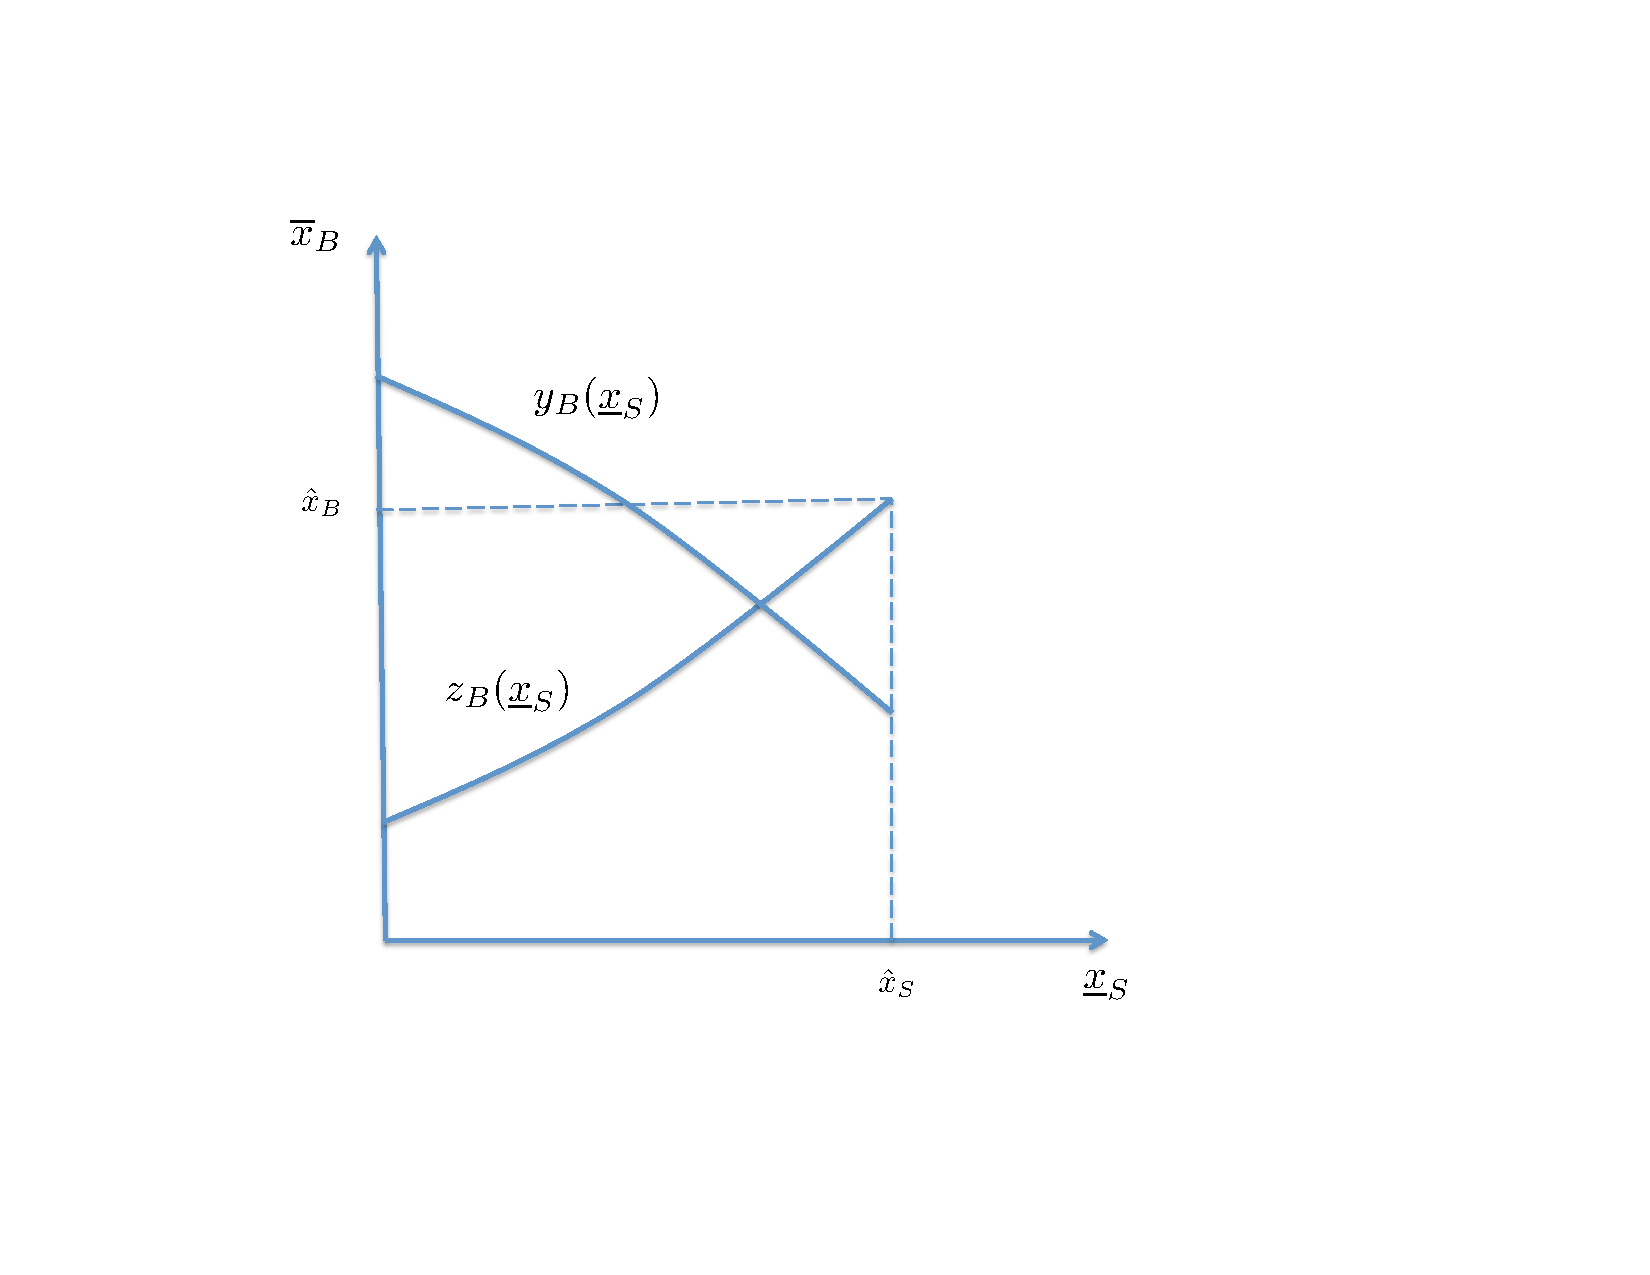
\includegraphics[scale = 0.6]{graphics/intersection.pdf}
  \caption{Functions $y_B(\cdot)$ and $z_B(\cdot)$.}
  \label{fig:intersection}
\end{figure}


Thus $y_B(\ul x_S)$ and $z_B(\ul x_S)$ are both continuous, and are,
respectively, decreasing and increasing functions. Continuing with the
proof, let $\hat x_S = X_S^*(v_J)$ and $\hat x_B = X_B^*(v_J)$ be the
bank's and broker's types in the bank-seller equilibrium ($v_J =
0$). The lower cutoff values are restricted between the lowest
possible value $0$, and $\hat x_S$. Both mapping $y_B(\cdot)$ and
$z_B(\cdot)$ are defined on the domain $[0,\hat x_S ]$.



Since the $\hat x_B$ type breaks even if the bank drops out at $v_J$
in the bank-seller equilibrium ($v_J = 0$), we must have $H(\hat
x_S,\hat x_B)>0$. The monotonicity of $H(\underline x_S,\ol x_B)$ in
$\ol x_B$ implies $z_B(\hat x_S)<\hat x_B$. At the same time, the
definition of $y_B(\cdot)$ implies $\hat x_B = y_B(\hat x_S)$, and it
follows that $z_B(\hat x_S)<y_B(\hat x_S)$.  Refer to
Figure~\ref{fig:intersection}. In view of the monotonicity of
$y_B(\cdot)$ and $z_B(\cdot)$, there are two possibilities. First, if
$z_B(0) \geq y_B(0)$, then type-$0$ bank prefers to bid $\ul p$ rather
than $v_J$. In this case, the curves $y_B(\ul x_S)$ and $z_B(\ul x_S)$
have a unique intersection given by
\begin{align}
  \ol x_B = y_B(\underline x_S)=z_B(\underline
  x_S), \label{eq:intersection}
\end{align}
with $\ol x_S \in (0,\hat x_S)$. If, on the other hand, $z_B(0) <
y_B(0)$, then type-$0$ bank prefers to bid $v_J$, so that the
equilibrium involves $\ol x_B = 0$ and the bunching extends all the
way to $x_S = 0$.
%
% The equilibrium cutoffs $\underline x_S$ and $\ol x_B$ are given by
% the intersection of the graphs of $y_B(\cdot)$ and $z_B(\cdot)$,


\end{proof}

% \section{Average Bidding Function in the Presence of
% Heterogeneity}\label{sec:avg-bid-heterogeneity}
%
% It may be reasonable to expect that even for non-securitized
% mortgages, some properties are better characterized by symmetric
% information. So as before, assume that a certain fraction of
% properties corresponds to symmetric information ($\alpha = 0$),
% while the remaining properties are better described by asymmetric
% information ($\alpha = 1$). The parameter $\alpha$ represents
% unobserved heterogeneity (to the econometrician). Then
% \begin{align*}
%   G_S^w(p_S(x_S;\alpha)|\alpha) = F_S(x_S|\alpha), \quad\quad \alpha
%   \in \{ 0,1 \}
% \end{align*}
% Averaging over the values of $\alpha$, we have (keeping in mind that
% $p_S(x_S; 0) = p_S^0(x_S)$ and $p_S(x_S;1) = p_S(x_S)$ in our
% previous notation),
% \[
% G_S^w(p_S^0(x_S)|0)\mathbbm P(\alpha = 0) +
% G_S^w(p_S(x_S)|1)\mathbbm P(\alpha = 1) = F_S(x_S)
% \]
% Since the signalling premium implies $p_S^0(x_S) < p_S(x_S) $, it
% follows that there exists $\hat p_S(x_S)$,
% \[ p_S^0(x_S) < \hat p_S(x_S) < p_S(x_S) \] such that
% \[ \hat p_S(x_S) = G_S^{w-\mathbbm 1}(F_S(x_S)) \] and Hypothesis
% \ref{hyp:sp} continues to hold, except that the identifiable object
% $G_S^{w-\mathbbm 1}(F_S(x_S))$ is now interpreted as $\hat
% p_S(x_S)>p_S^0(x_S)$.
%%

\end{document}
